%%%%%%%%%%%%%%%%%%%%%%%%%%%%%%%%%%%%%%%%%%%%%%%%%%%%%%%%%%%%%%%%%%%%%%%%%%%%%%%%
% Preámbulo                                                                    %
%%%%%%%%%%%%%%%%%%%%%%%%%%%%%%%%%%%%%%%%%%%%%%%%%%%%%%%%%%%%%%%%%%%%%%%%%%%%%%%%

\documentclass[11pt,a4paper,titlepage,twoside,openright,openbib]{report}
\usepackage{csquotes}
%\usepackage[
%bookmarksopen,
%bookmarksdepth=2,
%breaklinks=true
%]{hyperref}
%\PassOptionsToPackage{hyphens}{url}\usepackage{hyperref}
\usepackage[hyphens]{url}
\usepackage{hyperref}
\usepackage[section]{placeins}
\usepackage{lscape}
\makeatletter
\newcommand{\setword}[2]{%
  \phantomsection
  #1\def\@currentlabel{\unexpanded{#1}}\label{#2}%
}
\makeatother
%%% RELACIÓN DE VARIABLES A PERSONALIZAR %%%
%\def\lingua{gal}
\def\lingua{esp} % descomenta esta liña se redactarás a memoria en español
%\def\lingua{eng} % descomenta esta liña se redactarás a memoria en inglés
\def\nome{Amaro Castro Faci}                             % substitúe aquí o teu nome
\def\nomedirectorA{Antonio Daniel López Rivas}             % substitúe aquí o nome de quen dirixe
\def\nomedirectorB{Jose Carlos Dafonte Váquez}
\def\titulo{PESCI: Plataforma de Entrega de Servicios Cloud para Investigación} % substitúe aquí o título do teu TFG  % descomenta a mención correspondente
%\def\mencion{COMPUTACIÓN}
%\def\mencion{ENXEÑARÍA DO SOFTWARE}
%\def\mencion{ENXEÑARÍA DE COMPUTADORES}
%\def\mencion{SISTEMAS DE INFORMACIÓN}
\def\mencion{TECNOLOXÍAS DA INFORMACIÓN}

%\def\renomearcadros{si} % descomenta esta liña se redactas a memoria en español e prefires que
                         % os "cuadros" e o "índice de cuadros" se renomeen
                         % a "tablas" e "índice de tablas" respectivamente

\usepackage{estilo_tfg}

% Lista de paquetes potencialmente interesantes (uso baixo demanda)

% \usepackage{alltt}       % proporciona o entorno alltt, semellante a verbatim pero que respecta comandos
% \usepackage{enumitem}    % permite personalizar os entornos de lista
% \usepackage{eurofont}    % proporciona o comando \euro
% \usepackage{float}       % permite máis opcións para controlar obxectos flotantes (táboas, figuras)
% \usepackage{hhline}      % permie personalizar as liñas horizontais en arrays e táboas
% \usepackage{longtable}   % permite construir táboas que ocupan máis dunha páxina
% \usepackage{lscape}      % permite colocar partes do documento en orientación apaisada
% \usepackage{moreverb}    % permite personalizar o entorno verbatim
% \usepackage{multirow}    % permite crear celdas que ocupan varias filas da mesma táboa
% \usepackage{pdfpages}    % permite insertar ficheiros en PDF no documento
% \usepackage{rotating}    % permite diferentes tipos de rotacións para figuras e táboas
% \usepackage{subcaption}  % permite a inclusión de varias subfiguras nunha figura
% \usepackage{tabu}        % permite táboas flexibles
% \usepackage{tabularx}    % permite táboas con columnas de anchura determinada

%%%%%%%%%%%%%%%%%%%%%%%%%%%%%%%%%%%%%%%%%%%%%%%%%%%%%%%%%%%%%%%%%%%%%%%%%%%%%%%%
% Corpo                                                                        %
%%%%%%%%%%%%%%%%%%%%%%%%%%%%%%%%%%%%%%%%%%%%%%%%%%%%%%%%%%%%%%%%%%%%%%%%%%%%%%%%

\begin{document}

 %%%%%%%%%%%%%%%%%%%%%%%%%%%%%%%%%%%%%%%%
 % Preliminares do documento            %
 %%%%%%%%%%%%%%%%%%%%%%%%%%%%%%%%%%%%%%%%

 \begin{titlepage}
  
  \hspace*{128pt}
  \textcolor{udcpink}{{\fontencoding{T1}\fontfamily{phv}\selectfont Facultade de Informática}}\\[-32pt]

  \begin{center}
    
\includegraphics[scale=0.3]{imaxes/udc}\\[35pt]

    {\large TRABALLO FIN DE GRAO \\
            GRAO EN ENXEÑARÍA INFORMÁTICA \\
            MENCIÓN EN \mencion } \\[100pt]
    
    \begin{huge}
      \begin{spacing}{1.3}
        \bfseries \titulo
      \end{spacing}
    \end{huge}
  \end{center}
  
  \vfill
  
  \begin{flushright}
    {\large
    \begin{tabular}{ll}
      {\bf Estudante:} & \nome \\
      {\bf Dirección:} & \nomedirectorA \\ % COPIA E PEGA ESTA LIÑA MÁIS VECES SE O PRECISAS
    \end{tabular}}
  \end{flushright}
  \rightline{A Coruña, \datasimple\today.}
\end{titlepage}

 \iffalse
 \paxinaenbranco
 \dedicatoria{Dedicatoria} % escribe neste comando o teu texto de dedicatoria
 \paxinaenbranco
 \paxinaenbranco
 \begin{agradecementos}
 \blindtext % substitúe este comando polo teu texto de agradecementos
 \end{agradecementos}
 \paxinaenbranco
 \fi
 %%%%%%%%%%%%%%%%%%%%%%%%%%%%%%%%%%%%%%%%%%%%%%%%%%%%%%%%%%%%%%%%%%%%%%%%%%%%%%%%

\begin{abstract}\thispagestyle{empty}
  El Cloud Computing es un modelo que permite acceder a un conjunto de recursos, por ejemplo, redes, almacenamiento y cómputo, que pueden ser aprovisionados bajo demanda de forma automatizada y dinámica, reduciendo el coste del servicio para el usuario y el esfuerzo en cuanto a la administración de los recursos. El Centro de Investigación en Tecnoloxías da Información e as Comunicacións (CITIC) de la Universidade da Coruña cuenta con una infraestructura ideada para ofrecer un servicio de Cloud Computing a la comunidad universitaria. Este servicio consiste en que los usuarios pueden aprovisionar un conjunto de recursos del tamaño que requieran para realizar tareas que no serían posibles en dispositivos convencionales. Actualmente ese servicio está activo pero de forma limitada y no abierta a todos los usuarios del CITIC debido a que no existe una plataforma que permita gestionar los perfiles de usuario y su autenticación, ni un portal de acceso para aprovisionar recursos y gestionarlos de forma automatizada. En la actualidad, las tareas de aprovisionamiento y gestión de usuarios se realizan bajo petición previa al administrador del sistema que las ejecuta de forma manual lo cual produce gran coste en tiempo y recursos y aumenta los riesgos del servicio.\\
   El objetivo principal de este proyecto es desplegar un servicio Cloud en el CITIC usando como base las herramientas que ya se encuentran sobre la infraestructura, donde cada usuario pueda tener su un espacio donde gestionar la obtención de recursos y que permita reducir las tareas de administración al integrar el sistema de autenticación de la UDC y al automatizar los procesos de aprovisionamiento, permitiendo establecer unos límites y controlar los recursos que utiliza cada usuario. Todo esto con el fin de mejorar la eficiencia de la infraestructura.\\
   Para evitar problemas en el entorno de producción, el proyecto se desarrollará en un entorno de pruebas para mostrar las funcionalidades y características de la solución implementada pero que tendrán menor rendimiento que el entorno real por contar con recursos reducidos. El proceso se realizará siguiendo la metodología incremental Scrum en la cual primero se analizarán las diferentes alternativas disponibles y posteriormente se irán desplegando componentes para añadir nuevas funcionalidades que completen los objetivos del proyecto.
    % El Cloud Computing es un modelo que permite acceder a un conjunto de recursos, como por ejemplo, redes, almacenamiento, aplicaciones, servicios y potencia de cálculo, que pueden ser aprovisionados bajo demanda de una forma rápida sencilla, reduciendo el coste del servicio para el usuario y el esfuerzo en cuanto a gestión de los recursos.\\
  %  El Centro de Investigación en Tecnoloxías da Información e as Comunicacións (CITIC) de la Universidade da Coruña cuenta con una infraestructura ideada para ofrecer un servicio de Cloud Computing a la comunidad universitaria. Este servicio consiste en que los usuarios pueden aprovisionar un conjunto de recursos, que se traducen en máquinas virtuales, del tamaño que necesiten para realizar tareas que no serían posibles en dispositivos convencionales.\\
    % Actualmente el servicio está activo pero de forma limitada y no abierta a todos los usuarios del CITIC debido que no existe una plataforma que habilite el acceso a cada usuario a sus recursos, que gestione la autenticación de los usuarios, y que automatice y simplifique los procesos de aprovisionamiento de recursos. Hasta ahora, las tareas de aprovisionamiento y gestión de usuarios se realizan bajo petición previa al administrador del sistema y se ejecutan de forma manual lo cual consume más tiempo, recursos, y aumenta los riesgos sobre el servicio.\\
    % El objetivo principal de este proyecto es desplegar un servicio Cloud en el CITIC usando como base las herramientas que ya se encuentran sobre la infraestructura, donde cada usuario pueda tener su propio espacio donde poder gestionar sus recursos según sus necesidades y de forma simple y dinámica, que simplifique la gestión de usuarios integrando el sistema de autenticación de la UDC en el servicio, y establecer un sistema de valoración de los recursos para poder controlar y limitar la cantidad de recursos que un usuario puede aprovisionar para mejorar el uso y funcionamiento del servicio. En definitiva, el objetivo es desplegar un entorno Cloud que haga la infraestructura física más eficiente y para entregar todo su potencial.
  \vspace*{20pt}
\begin{multicols}{2}
\begin{description}
\item [\palabraschaveprincipal:] \mbox{} \\[-20pt]
  \blindlist{itemize}[7] % substitúe este comando por un itemize
                         % que relacione as palabras chave
                         % que mellor identifiquen o teu TFG
                         % no idioma principal da memoria (tipicamente: galego)
\end{description}
\begin{description}
\item [\palabraschavesecundaria:] \mbox{} \\[-20pt]
  \blindlist{itemize}[7] % substitúe este comando por un itemize
                         % que relacione as palabras chave
                         % que mellor identifiquen o teu TFG
                         % no idioma secundario da memoria (tipicamente: inglés)
\end{description}
\end{multicols}

\end{abstract}

%%%%%%%%%%%%%%%%%%%%%%%%%%%%%%%%%%%%%%%%%%%%%%%%%%%%%%%%%%%%%%%%%%%%%%%%%%%%%%%%

 \paxinaenbranco

 \pagenumbering{roman}
 \setcounter{page}{1}

 \tableofcontents
 \listoffigures
 \listoftables
 \cleardoublepage
 
 \pagenumbering{arabic}
 \setcounter{page}{1}
 \bstctlcite{IEEEexample:BSTcontrol}

 %%%%%%%%%%%%%%%%%%%%%%%%%%%%%%%%%%%%%%%%
 % Capítulos                            %
 %%%%%%%%%%%%%%%%%%%%%%%%%%%%%%%%%%%%%%%%

 \chapter{Introdución}
\label{chap:introducion}

\lettrine{P}{rimer} capítulo da memoria, onde xeralmente se exporán as
liñas mestras do traballo, os obxectivos, etc. Incluimos un par de
exemplos de citas~\cite{ErlangBook,ErlangWebBook} e de referencias
internas (sección \ref{sec:mostra}, páxina \pageref{sec:mostra}).

\Blindtext

\section{Sección de mostra}
\label{sec:mostra}

\Blindtext

\subsection{Subsección de mostra}

\Blindtext

 \begin{chapter}{Estado de los recursos}
\label{chap:estado-recursos-CITIC-VCF}

\lettrine{C}{on} el fin de contextualizar los recursos utilizados para el desarrollo del proyecto, en este capítulo se expone la situación actual de la infraestructura situada en el CITIC. Esto incluye el software que está en funcionamiento, los recursos físicos de los que se compone, y el estado actual de las herramientas que rodean a dichos recursos.

\begin{section}{Infraestructura}

    La infraestructura física donde se encuentra el servicio de virtualización, se encuentra en el edificio del CITIC de la UDC, dentro de un rack alojado en su Centro de Proceso de Datos (CPD)\cite{citicUDC}.
% La infraestructura física donde se planea desplegar el servicio de virtualización, se encuentra localizada en el edificio del CITIC de la UDC, dentro de un rack alojado en su Centro de Proceso de Datos (CPD)\cite{citicUDC}. 
\begin{subsection}{Cómputo}
    Está formada por 5 hosts Lenovo NeXtScale nx360 M5, cada uno con dos procesadores Intel Xeon E5-2650, 128 GB de memoria RAM y una tarjeta gráfica Tesla M60,  y 3 hosts Dell EMC PowerEdge R740 cada uno con dos procesadores Xeon Gold 6146, 384 GB de memoria RAM y una tarjeta gráfica Tesla P40. Todos ellos aportan flexibilidad en cuanto a que permiten escalar la infraestructura y ofrecen gran rendimiento de cómputo.
\end{subsection}
\begin{subsection}{Almacenamiento}
    El sistema de almacenamiento está colocado físicamente en la misma ubicación que los hosts pero en su abstracción lógica este es independiente y está separado de cada host. Está conformado por 13 discos duros SSD de 3.84 TB de capacidad, obteniendo así una cantidad total de casi 50 TB, pero su capacidad útil es de 34 TB ya que se utiliza la configuración de almacenamiento RAID 5 para aporta mayor integridad de los datos, mayor tolerancia a fallos y mayor ancho de banda. Los discos duros están colocados en una misma cabina formando un \textit{pool} de almacenamiento que se divide en cinco LUNs (Logical Storage Unit) de 2 TB cada una, representadas en el software de virtualización como cinco datastores, y que emplean el sistema de archivos VMFS propio de la compañía VMware, el cual optimiza el almacenamiento de máquinas virtuales.
    La configuración y gestión de este sistema se tiene que realizar al nivel de la capa física, por lo tanto si se quiere realizar un despliegue en el sistema de virtualización que requiera una configuración de almacenamiento diferente a la existente, como por ejemplo un sistema RAID con diferentes características, sería necesario modificar la configuración del sistema físico, siendo muy costoso en tiempo y riesgos. Por lo tanto, este sistema de almacenamiento no permite ajustar de forma precisa, rápida y bajo demanda la configuración de almacenamiento que un usuario requiera para sus aplicaciones.
\end{subsection}

\begin{subsection}{Red}
    El sistema de almacenamiento forma una Storage Area Network (SAN), para ello se utilizan conexiones de tipo 10 Gbit entre los hosts y las cabinas donde se encuentran los discos duros. Para soportar este tipo de conexiones, cada cabina incorpora dos controladores con conectores de tipo SFP+. Además, las cabinas de almacenamiento incorporan otros dos puertos de 1 Gbit para llevar a cabo la administración de los discos. En esta estructura se utilizan los protocolos de red Ethernet y iSCSI. Para mantener la disponibilidad del acceso al sistema de almacenamiento y aumentar la disponibilidad de de las conexiones entre hosts, cada host de ellos se conecta a dos switches \textit{trunk} para establecer rutas redundantes.
    Igual que con el sistema de almacenamiento, si se requieren realizar modificaciones sobre la red para adaptarse a los requisitos de un determinado despliegue, habría que hacerlas directamente sobre la red física. Esto puede generar problemas en la conectividad del entorno a parte de generar gran coste de tiempo.

\end{subsection}

\end{section}

\begin{section}{Software}
    \label{subsec:softwareinstalado}
    Actualmente, el software desplegado sobre la infraestructura está formado por los productos de la compañía VMware, uno de los principales proveedores de software de virtualización. Todos los componentes instalados se engloban dentro del producto \textbf{VMware vSphere}, en su versión 6.7, el cual contiene lo necesario para virtualizar la infraestructura junto con las herramientas para entregar el servicio y gestionar la infraestructura virtual. A continuación	se describen los principales componentes que tiene VMware vSphere y que están instalados en la infraestructura.
    % principal componente ya que se utiliza para virtualizar parte de la infraestructura física y proporcionar las herramientas necesarias para gestionarla, sus principales componentes internos se describen a continuación.
    \begin{figure}[h]
        \centering
        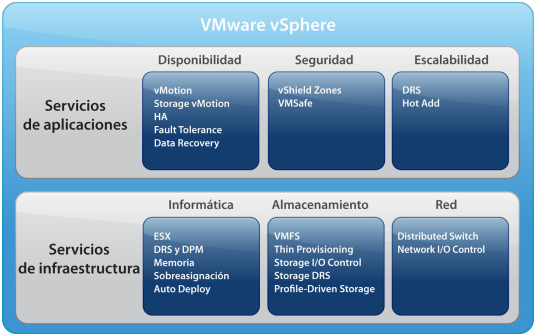
\includegraphics[width=0.75\textwidth]{imaxes/cap2recursos/contentVSphere}
        \caption{Componentes de VMware vSphere\cite{fotovSphere}}
        \label{fig:vSphere-components}
    \end{figure}
    \FloatBarrier
    En cada host está instalado el hipervisor ESXi de tipo baremetal, este se encarga de habilitar la virtualización de los recursos. Sobre los hosts se ecuentra una VM que alberga el servicio VMware vCenter Server, el cual actúa como centro de administración de todas las máquinas virtuales (VMs) y hosts que forman la infraestructura. Además, esta instancia de VMware vCenter Server contiene una instancia embebida de Platform Services Controller (PSC), punto que centraliza la autenticación en las APIs de VMware vCenter Server, actúa como servidor de licencias y contiene servicio de autenticación de usuarios llamado vCenter Single Sign-On, este último se utiliza para gestionar la autenticación de los usuarios registrados en VMware vCenter Server. El acceso e interfaz de VMware vCenter Server la proporciona el componente vSphere Web Client, una página web donde el usuario puede autenticarse y gestionar las VMs y hosts que forman el entorno y el resto de servicios de VMware vSphere. Además, incorpora vSphere Update Manager desde el cual se gestionan las actualizaciones de los componentes de VMware vSphere. Para administrar las conexiones de las VMs desplegadas en el entorno, se utiliza el componente vSphere Distributed Switch (vDS), un switch virtual donde se establecen puertos para que las VMs tengan acceso a la red y a través de los cuales se configuran las propiedades del tráfico. Finalmente, se utilizan varios servicios de gran importancia para mantener la disponibilidad de las VMs desplegadas en la infraestructura:
    
    \begin{itemize}
        \item vMotion: encargado de migrar VMs de un host a otro de forma transparente y sin detener su ejecución ni el servicio.
        
        \item vSphere High Availability (HA): encargado de recuperar el servicio de una VM que ha sufrido un fallo. Para ello, la VM es reiniciada en otro host del entorno.
        % En caso de que una VM deje de estar activa, este servicio intenta encenderla de forma automática en otro host del entorno. A diferencia de vMotion, este solo actúa en caso de que la VM o el host donde se encuentra la VM sufra un fallo y esta pase a estar no disponible. 
        
        \item vSphere Distributed Resource Scheduler (DRS): encargado de balancear la carga de trabajo entre los hosts disponibles en el entorno, migrando las VMs cuando sea necesario para maximizar el rendimiento de la infraestructura. 
        
        % vSphere DRS genera recomendaciones sobre donde se debería desplegar una máquina virtual durante su creación, utiliza vMotion para migrar las VMs y así maximizar el rendimiento o para manterner la VM activa durante tareas de mantenimiento en un host. vSphere DPM se encarga de gestionar el consumo de energía de cada host según el rendimiento actual. Sotrage DRS se encarga de balancear la carga de almacenamiento y las operaciones de lectura y escritura entre los \textit{datastores} disponibles.
        
        % \item \textbf{vSphere Fault Tolerance}: gestiona una copia de todos los archivos y discos de cada VM sincronizada con los archivos originales. Este servicio usado con vSphere HA y vSphere DRS proporciona recuperación ante fallos automática y disponibilidad continua de las VMs, sin perdida de datos y sin pérdida de las conexiones establecidas. En caso de que una VM deje de estar disponible esta se reinicia en un host diferente. Este servicio está orientado a proteger aquellas tareas que requieren un alto rendimiento o que son críticas.
    \end{itemize}
\end{section}

\begin{figure}[hp]
    \centering
    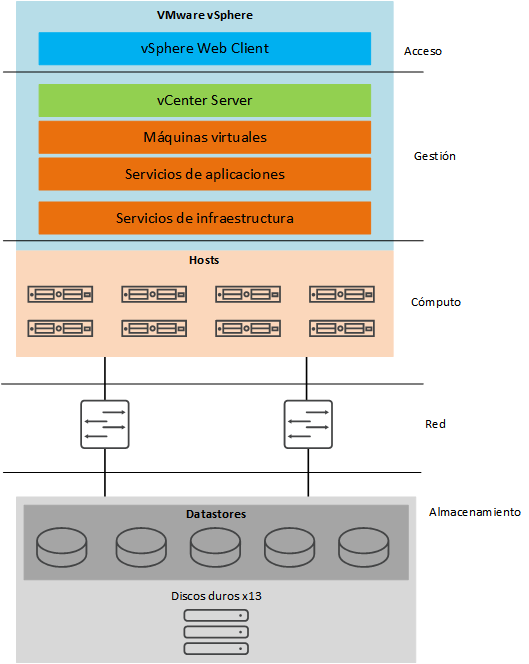
\includegraphics[width=0.6\textwidth]{imaxes/cap2recursos/recursosReal.png}
    \caption{Componentes físicos y software que forman la infraestructura actual.}
    \label{fig:infrastructure-components-production}
\end{figure}
\FloatBarrier

% \begin{section}{Estado de la tecnología}
% Con el desarrollo de las tecnologías web y la comercialización por parte de grandes empresas de su infraestructura, los servicios \textit{Infrastructure as a Service} (IaaS) han ganado una popularidad considerable, con ello también se han desarrollado herramientas software dedicadas a la gestión de infraestructura para la implementación de sistemas Cloud Computing. Algunas de estas son VMware Cloud Foundation (creado en 2011), OpenStack (creado en 2010) o Apache CloudStack (creado en 2012). Estos productos proveen software que permite construir una infraestructura virtualizada sobre un conjunto de recursos físicos, con el objetivo de separar la administración de la capa física de la capa virtual, y simplificar y automatizar la gestión y escalabilidad de los recursos. Proponen un modelo que persigue reducir costes de gestión de la infraestructura y aumentar la disponibilidad del servicio, es decir, aumentar la eficiencia de la infraestructura física.

% Como ya se ha visto, en el mercado existen varias alternativas que se pueden utilizar para cumplir los objetivos del proyecto. Finalmente, se ha escogido el producto \textbf{VMware Cloud Foundation} (VCF) ya que se integra perfectamente con los componentes de VMware ya instalados en la infraestructura y, por lo tanto, su mantenimiento sencillo. Desplegar un producto de una compañía diferente e integrarlo con los elementos desplegados en el CITIC, podría producir problemas de compatibilidad entre versiones a largo plazo, a pesar de que este se pueda integrar con el software VMware vSphere. Utilizando los productos de un mismo proveedor se asegura el soporte del software instalado y la obtención del máximo rendimiento de cada componente.
% Para poder usar este software es necesaria la adquisición de licencias. Estas se organizan por componente y por número de hosts sobre los que se va a instalar el producto. Aunque tienen un coste elevado, este producto aporta grandes beneficios.

% \begin{subsection}{VMware Cloud Foundation}

%     Esta solución de VMware virtualiza todas las capas de la infraestructura combinando cuatro de sus productos. Utiliza \textbf{VMware vSphere} para virtualizar y gestionar el cómputo, \textbf{VMware vSAN} para virtualizar y gestionar el almacenamiento, \textbf{VMware NSX-T} para la virtualización y gestión de la red, y \textbf{VMware vRealize Suite} para gestionar las operaciones de la infraestructura virtual como el aprovisionamiento de recursos. Todos estos servicios juntos convierten el CPD en un Software Defined Datacenter (SDDC), un entorno donde existe una infraestructura física que se abstrae en una capa virtual para separar la gestión de ambas y poder modificar la infraestructura virtual según las necesidades de los usuarios sin necesidad de modificar la configuración de la infraestructura física, y que permite a los usuarios aprovisionar recursos, construyendo así un servicio de Cloud Computing. Con esta estructura se obtienen las siguientes características:
    
% \begin{itemize}

%     \item Servicios software con integración nativa: ofrece un conjunto de servicios software para el almacenamiento, red, seguridad y gestión del servicio Cloud. Estos servicios se integran de forma nativa con la infraestructura minimizando las tareas de configuración y administración.

%     \item Escalabilidad y elasticidad de los recursos: la capacidad de la infraestructura se puede modificar de forma sencilla gracias a la automatización del ciclo de vida de todos los elementos y al desacople entre las dos capas (la física y la virtual).

%     \item Supervisión de los recursos: monitoriza los recursos con reconocimiento de aplicaciones y solución de problemas, permitiendo conocer todos los eventos que tienen lugar en la infraestructura. También permite establecer políticas de seguridad en cuanto al acceso a los recursos y la red.

%     \item Aprovisionamiento automatizado: permite la obtención de recursos de forma automática incluyendo servicios de red, almacenamiento y cómputo. Los componentes de la infraestructura virtualizada se encargan de la reserva de los recursos y de todas las operaciones necesarias para llevarla acabo.

%     \item Ciclo de vida automatizado: automatiza las operaciones de gestión previas, iniciales y posteriores de la plataforma para simplificar y coordinar su gestión. En estas tareas incluye el despliegue de la plataforma y su implementación, la escalabilidad de los recursos físicos y la instalación de actualizaciones para cada componente software.

% \end{itemize}
% \begin{figure}[h!]
%     \centering
%     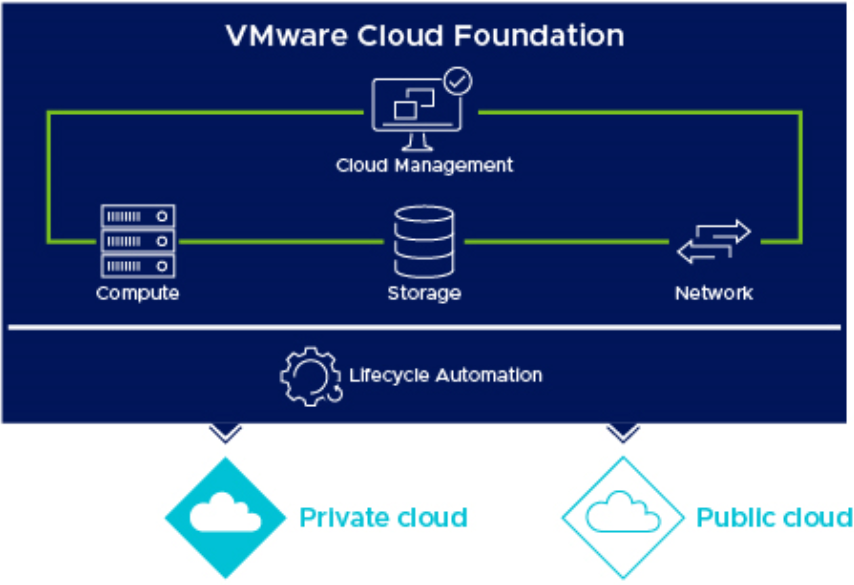
\includegraphics[width=0.6\textwidth]{imaxes/cap2recursos/overviewCF.png}
%             \caption{Estructura de VMare Cloud Foundation.}
%     \label{fig:Cloud-Foundation-Overview}
%     \end{figure}
%     \FloatBarrier
%     \begin{figure}[h]
%         \centering
%         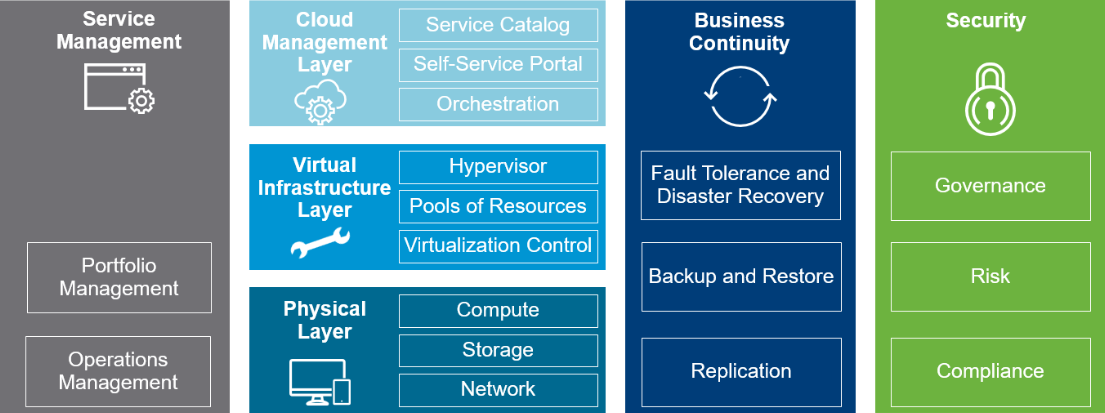
\includegraphics[width=0.8\textwidth]{imaxes/cap2recursos/SDDCoverview.png}
%         \caption{Elementos de un SDDC gestionado con VMware Cloud Foundation.}
%         \label{fig:layers-Sddc}
%     \end{figure}
%     \FloatBarrier
% \end{subsection}

% \begin{subsection}{Componentes de VMware Cloud Foundation}
% \label{subsubsect:cfcomponents}

% Ya se ha visto que VCF está formado por cuatro productos principales. En este apartado se describirán las características de esos cuatro componentes más el servicio que los coordina\footnote{Las características del componente VMware vSphere son las mismas que las descritas en el punto \ref*{subsec:softwareinstalado}}. Se utilizará la versión 4.0 de VMware Cloud Foundation lo cual implica que se implementarán las versiones\cite{componentesCloudFound} 4.0 de SDDC Manager, 7.0.0 de VMware vSphere, 7.0.0 de VMware vSAN, 3.0 de VMware NSX-T y 8.1 de VMware vRealize Suite.
% \begin{figure}[h]
%     \centering
%         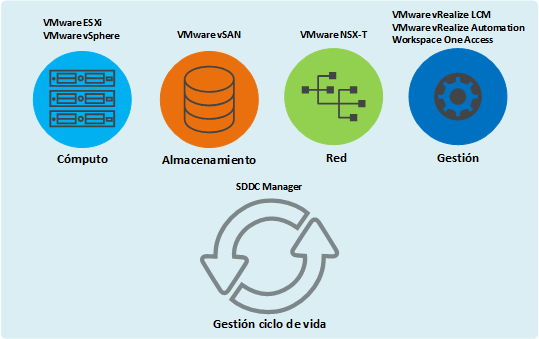
\includegraphics[width=0.6\textwidth]{imaxes/VCF-componentes/ComponentesVCF.png}
%         \caption{Partes de un SDDC y componentes de VCF que las implementan.}
%         \label{fig:componentes-funciones-VCF}
%     \end{figure}
%     \FloatBarrier
% \begin{subsubsection}{SDDC Manager}
%     SDDC Manager se encarga de gestionar el ciclo de vida de todos los componentes de VCF, esto incluye el despliegue de cada uno, su configuración y la obtención e instalación de actualizaciones. Centraliza la gestión de las licencias y certificados de cada componente y administra el aprovisionamiento de nuevos recursos físicos para el SDDC y los ya existentes.
% \end{subsubsection}

% \begin{subsubsection}{VMware vSAN}
%     VMware vSAN virtualiza el almacenamiento del SDDC. Permite gestionar de forma centralizada, desde la interfaz de vSphere Web Client, el sistema de almacenamiento sin necesidad de tener que modificar la configuración física. El sistema de almacenamiento se abstrae para formar único datastore sobre el que se establecen políticas de uso y disponibilidad. El acceso por parte de cada host al datastore se realiza con el protocolo IP, a través de una subred dedicada al servicio. Con VMware vSAN, el datastore está formado por discos de almacenamiento que se organizan en grupos que se asignan a un host. Los grupos pueden tener configuración \textit{Hybrid}, que combina discos HDD y SDD, o configuración \textit{All-Flash} que solo utiliza SSD y por lo tanto tiene mayor rendimiento. Dentro de cada grupo existe un disco de caché y al menos un disco de capacidad donde se almacenan los datos persistentes\cite{operacionesVSAN}. 
%     % En el modo \textit{All-Flash}\footnote{Solo se describe el modo \textit{All-Flash} porque es la configuración recomendada por VMware.} la operación de lectura se realiza directamente sobre los discos de capacidad y la operación de escritura se hace sobre el disco caché que posteriormente escribe los datos en el disco de capacidad.
    
%     \begin{figure}[h]
%     \centering
%         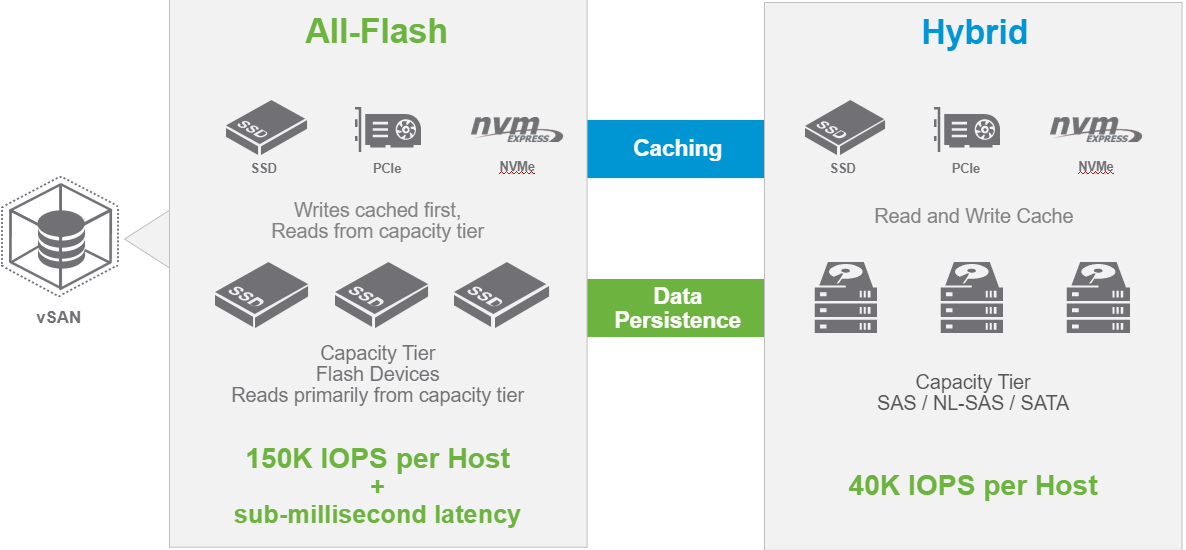
\includegraphics[width=0.6\textwidth]{imaxes/cap2recursos/rendimientoVSAN.png}
%         \caption{Configuración \textit{All-Flash} y configuración \textit{Hybrid} en vSAN}
%         \label{fig:performance-Hybrid-AllFlash-vSAN}
%     \end{figure}
%     \FloatBarrier
% \end{subsubsection}

% \begin{subsubsection}{VMware NSX-T}
%     VMware NSX-T virtualiza la red del SDDC. Abstrae los componentes físicos de la red para generar una red virtual desacoplada de la infraestructura física, esta se configura sin modificar la red física y para ello aporta servicios de red virtualizados y la posibilidad de crear y extender subredes sobre la infraestructura. Internamente tiene tres componentes, NSX-T Manager, NSX-T Controller y NSX-T Edge. El primero, es el punto de acceso a la configuración de VMware NSX-T y el que almacena y transmite la configuración establecida, el segundo controla las redes y se encarga de informar sobre el estado y la configuración de las redes virtuales. El último componente, NSX-T Edge, proporciona servicios de red y enrutamiento a las redes virtuales. Los hosts que están integrados en VMware NSX-T se encargan de controlar el tráfico y monitorizar las conexiones que mantiene VMware NSX-T.
%     % El control del tráfico y la monitorización de las conexiones se hace desde el componente \textbf{Transport Node} (TN) con la información que recibe de las instancias de NSX-T Controller. Existen dos tipos de TNs, \textbf{Hypervisor Transport Node} que son hosts con ESXi instalado y que están configurados para correr los servicios de VMware NSX-T, y \textbf{NSX-T Edge Node} que se trata de una \textit{appliance} instalada en una VM o sobre un host físico para proveer un conjunto de servicios de red centralizados para las redes virtuales de VMware NSX-T.
%     \begin{figure}[h!]
%         \centering
%             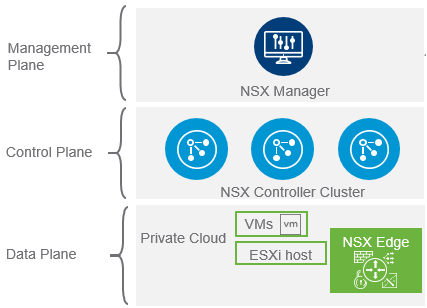
\includegraphics[width=0.6\textwidth]{imaxes/VCF-componentes/nsx-t-layers.png}
%             \caption{Componentes de VMware NSX-T y capas en las que se dividen}
%             \label{fig:nsx-t-components}
%         \end{figure}
%         \FloatBarrier
% \end{subsubsection}

% \begin{subsubsection}{VMware vRealize Suite}
%     VMware vRealize Suite agrupa un conjunto de productos que si bien no son obligatorios para desplegar VCF, aportan funcionalidades extra que completan la formación del SDDC y del servicio Cloud. Los productos que se utilizarán en este proyecto son \textbf{vRealize Suite Lifecycle Manager} dedicado a gestionar el despliegue, actualizaciones, certificados y licencias de los productos que forman VMware vRealize, \textbf{Workspace One Access} dedicado a gestionar los usuarios y ser el punto de acceso centralizado de las aplicaciones de VMware vRealize Suite y, finalmente, \textbf{vRealize Automation} el cual permite a los usuarios del SDDC diseñar y aprovisionar un conjunto de recursos de la infraestructura según sus necesidades y de forma automatizada mientras el administrador puede limitar la cantidad de recursos que se consumen.
% \end{subsubsection}

% \end{subsection}

% \end{section}

\end{chapter}
 \begin{chapter}{Planificación}
\label{chap:planificacionProyecto}
\lettrine{E}{n} este capítulo se propone una planificación del proyecto con el fin de organizar su estructura y exponer sus costes temporales y económicos aproximados necesarios para su realización.
\begin{section}{Tareas y costes del proyecto}
\underline{Tarea 1}. Analizar qué componentes hardware y software componen la infraestructura y cuales son sus funciones. En cuanto al hardware se comprueban las especificaciones concretas de los recursos de cómputo, almacenamiento y red, y cómo están estructurados el sistema de almacenamiento y la red. Respecto al software se comprueba qué productos y servicios hay instalados y cuales son sus funciones dentro del entorno.\\
% \underline{Tarea 1}. Analizar como está formada la infraestructura, que componentes hardware y software la componen y cual es la función de cada uno de ellos. En cuanto a la parte física se comprueban las especificaciones concretas del hardware de cómputo, almacenamiento y red. También como están organizados y estructurados tanto el sistema de almacenamiento y la red de la infraestructura. En la parte de software, se detallan las funciones de los principales programas y servicios que están instalados en el entorno.\\
\underline{Tarea 2}. Analizar y seleccionar una herramienta de las disponibles en el mercado que se adapte a los objetivos del servicio que se quiere construir y a las características de la infraestructura. En este proceso se tiene en cuenta la compatibilidad con el software ya existente, el coste de mantenimiento y la eficiencia de las herramientas disponibles.\\
\underline{Tarea 3}. Tarea que agrupa las tareas dedicadas al proceso de configuración de la infraestructura e instalación y configuración de la herramienta seleccionada. Estas son las tareas 4, 5, 6, 7, 8, 9 y 10.\\
\underline{Tareas 4, 5, 6, 7, 8, 9 y 10.} Antes de realizar la instalación de la nueva herramienta es necesario comprobar sus requisitos software y hardware (tareas 4 y 5). También se deben establecer los parámetros de configuración iniciales que se van a aplicar a la nueva plataforma (tarea 6). Construcción de un entorno de pruebas con una infraestructura que se adapte a los requisitos de la herramienta seleccionada y así evitar problemas en el entorno real del CITIC (tareas 7 y 8). Una vez el entorno está preparado se efectúa el despliegue de la herramienta(tarea 9), posteriormente se configura y se comprueba el funcionamiento del nuevo servicio (tarea 10).\\
% \underline{Tareas 4, 5, 6, 7, 8, 9 y 10.} Con el objetivo de desplegar la herramienta seleccionada anteriormente se llevan a cabo las siguientes tareasComprobación de requisitos, preparación del entorno, establecimiento de parámetros configuración, despliegue de la plataforma sobre la infraestructura existente y configuración de la plataforma después del despliegue. Antes de realizar la instalación de la nueva herramienta es necesario comprobar sus requisitos necesarios para que las capacidades del servicio final se adapten a las necesidades de uso (tareas 4 y 5). También se deben establecer los parámetros de configuración iniciales que se van a aplicar a la nueva plataforma (tarea 6). Durante el proceso de comprobación de requisitos puede surgir la necesidad de realizar cambios sobre las capacidades de la infraestructura y la configuración de los componentes ya existentes en el entorno inicial para que este se adapte a los requisitos de la nueva plataforma (tareas 7 y 8). Una vez el entorno está preparado para la herramienta pueda ser instalada entonces se efectúa el despliegue (tarea 9), posteriormente se configura y se comprueba el funcionamiento del nuevo servicio (tarea 10).\\
\underline{Tarea 11.} Esta tarea marca el final del despliegue y configuración del nuevo servicio en la infraestructura.\\
\underline{Tarea 12}. Diseñar una integración de la nueva plataforma con el sistema de autenticación de la UDC para que los usuarios finales del servicio puedan autenticarse sin necesitar nuevas credenciales. Se debe utilizar un directorio de usuarios que simule el directorio de la UDC y así evitar problemas en el entorno de producción.\\
% \underline{Tarea 12}. Diseñar una integración de la nueva plataforma con el sistema de autenticación de la UDC para que los usuarios finales del servicio puedan autenticarse sin necesitar nuevas credenciales. Para ello es preciso comprobar el método de acceso al directorio de usuarios de la UDC y la forma de conectarlo con la plataforma desplegada para, posteriormente, realizar un diseño de la solución. Este proceso requiere realizar una solicitud de acceso a los servicios internos de la UDC.\\
\underline{Tarea 13}. Implementación y despliegue de la solución que permita integrar el directorio de usuarios del entorno de pruebas con la herramienta desplegada para la autenticación de usuarios con sus propias credenciales.\\
% \underline{Tarea 14}. Análisis del uso que harán los usuarios del servicio para establecer políticas sobre el uso de recursos. Para realizar este cálculo, primero se debe analizar el uso previo al despliegue del nuevo servicio que los usuarios hacen de la infraestructura y, después, estimar el uso que pueden llegar a realizar una vez el servicio sea accesible. Hay que tener en cuenta la cantidad de usuarios que lo utilizan, que lo van a utilizar y la cantidad de recursos que se emplean y que se van a emplear. Una vez obtenida una estimación, se realiza un diseño de las políticas que se van a aplicar.\\
\underline{Tarea 14}. Diseño de un sistema de facturación/valoración del consumo de recursos por parte de los usuarios con la intención de limitar la cantidad de recursos que un usuario puede aprovisionar, y así tener recursos disponibles para todos los usuarios y aumentar la eficiencia la eficiencia de la infraestructura.\\
% \underline{Tarea 15}. Diseño de un sistema de facturación/valoración de los recursos del servicio en base a las políticas de uso establecidas. Basándose en las políticas establecidas en la tarea 14, se debe pensar como se pueden aplicar sobre el servicio. Esto puede ser a través de una herramienta externa, en ese caso sería necesario realizar un desarrollo, o integrando la configuración en los parámetros de configuración de la plataforma.\\
% La intención de este sistema es limitar la cantidad de recursos que un usuario puede aprovisionar permitiendo aumentar la eficiencia de los recursos físicos reduciendo la cantidad de recursos ociosos.\\
\underline{Tarea 15}. Implementación y despliegue del sistema de facturación/valoración.\\
% \underline{Tarea 16}. Implementación y despliegue del sistema de facturación/valoración. Para implementar este sistema puede que sea necesario realizar el desarrollo de una herramienta si se determina que no es posible establecerlo a través de los parámetros de configuración de la plataforma. \\
\underline{Tarea 16, 17 y 18}. Recopilación de la información necesaria para la realización de cada tarea. La información de apoyo se debe obtener de documentaciones, artículos, vídeos o libros de  fuentes fiables como empresas desarrolladoras de los productos utilizados o expertos especializados. El objetivo la recopilación de información es obtener conocimiento sobre las herramientas con las que se está trabajando para luego tener una base que facilite la realización de las tareas descritas. Esto se realiza desde el comienzo del proyecto hasta su finalización para tener claros los conceptos que se desarrollan y para conocer los detalles del trabajo que se realiza.\\
\underline{Tarea 19, 20 y 21}. Redacción de la memoria del proyecto. Se escribe un documento con todos los detalles de todas las tareas realizadas durante el proyecto, incluyendo los cambios realizados en la infraestructura, las configuraciones establecidas y como se lleva a cabo cada proceso del proyecto. Su objetivo es transmitir el conocimiento adquirido durante su realización y proponer una solución para habilitar un servicio Cloud en la infraestructura del CITIC. La escritura de este documento se realiza a la vez que cada tarea para detallar los pasos realizados en cada caso, por lo que su duración es igual a la duración total de todo el proyecto.\\
% \underline{Tarea 20, 21 y 22}. Redacción de la memoria del proyecto. Se escribe un documento con todos los detalles de todas las tareas realizadas durante el proyecto, incluyendo los cambios realizados en la infraestructura, las configuraciones establecidas y como se lleva a cabo cada proceso del proyecto. Su objetivo es transmitir el conocimiento adquirido durante el proyecto sobre como realizar el despliegue de una plataforma de virtualización y los beneficios que esta puede tener. La escritura de este documento se realiza a la vez que completa cada tarea para detallar los pasos realizados en cada caso, por lo que su duración es igual a la duración total de todo el proyecto.\\

La duración total del proyecto se estima en 101 días. teniendo en cuenta que el estudiante trabaja durante 4 horas diarias. El coste mostrado en la figura \ref{fig:estadisticasproyecto} se refiere al coste correspondiente al estudiante si trabaja por 25 €/hora. 
\begin{figure}[h!]
  \centering
  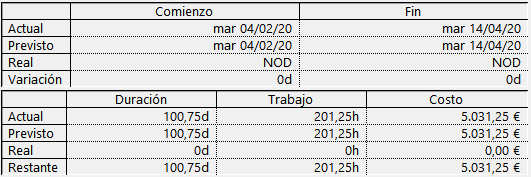
\includegraphics[width=1\textwidth]{imaxes/extras/estadisticasProyecto.png}
  \caption{Estadísticas sobre la planificación del proyecto.}
  \label{fig:estadisticasproyecto}
\end{figure}
\FloatBarrier
\begin{landscape}
\begin{figure}[hp]
  \centering
  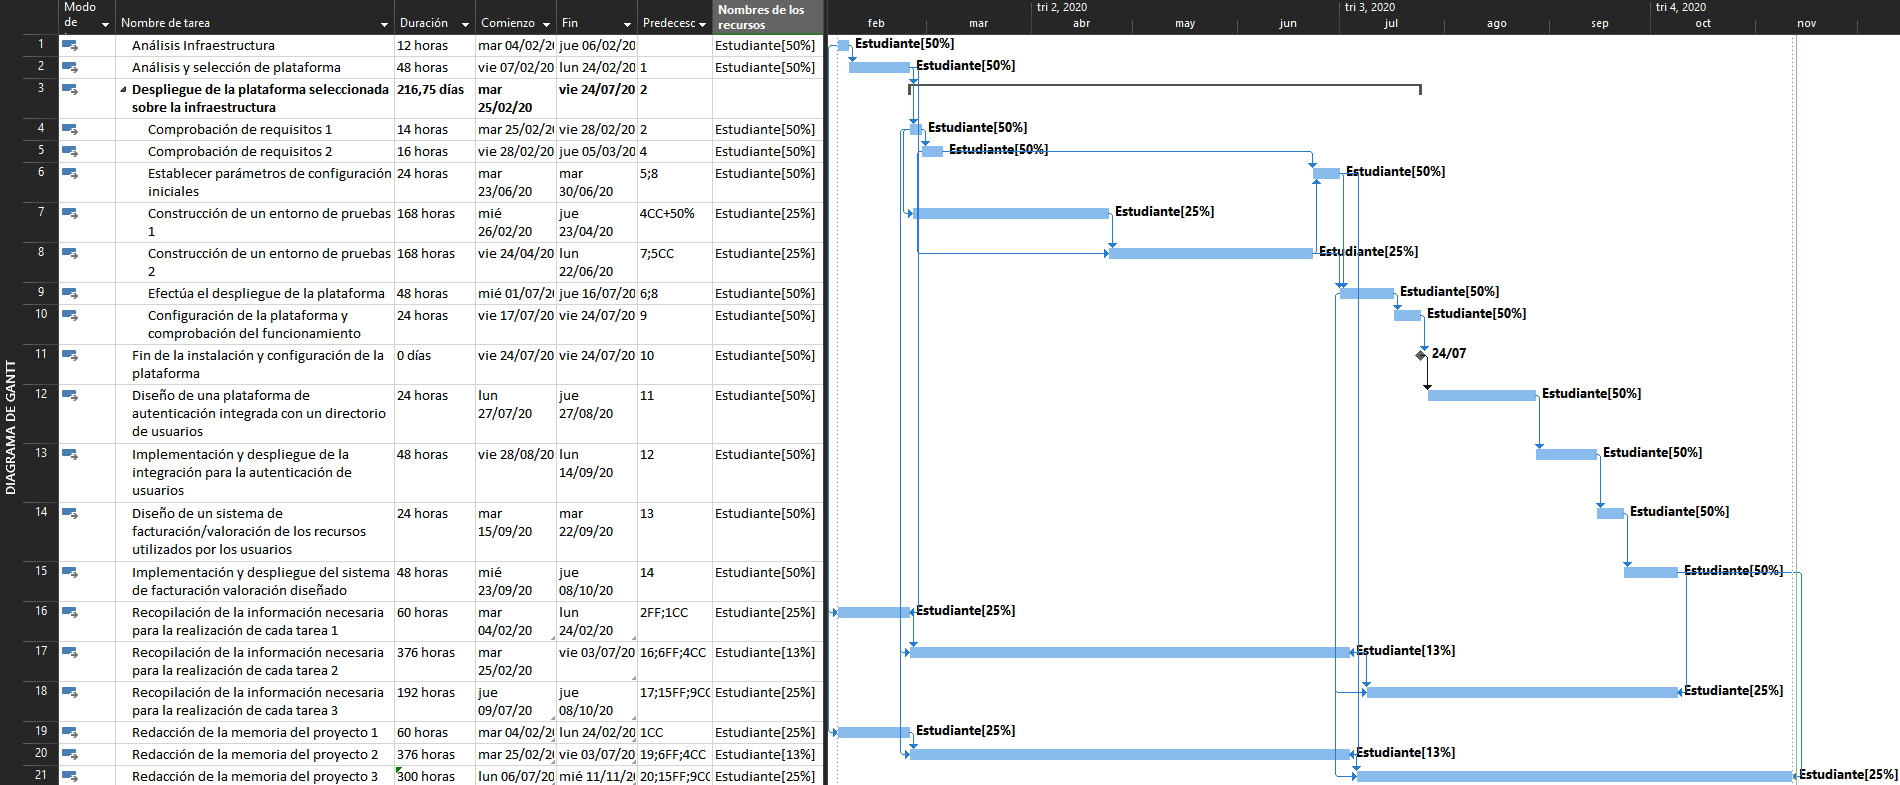
\includegraphics[width=1.5\textwidth]{imaxes/extras/diagramaGranttt.png}
  \caption{Diagrama de Grantt sobre la planificación del proyecto.}
  \label{fig:tareasproyecto}
\end{figure}
\end{landscape}
\FloatBarrier
\end{section}

% \begin{section}{Costes de implementación}
% Los principales costes de implementar la solución propuesta en la infraestructura de producción del CITIC son aquellos relacionados con los trabajadores que lo llevan a cabo y las licencias necesarias para cada componente de VMware Cloud Foundation\footnote{Los componentes que se especifican son aquellos que son obligatorios para desplegar VMware Cloud Foundation.}.\\
% Cada componente de VMware Cloud Foundation requiere su propia licencia\cite{licenses}. El precio de cada licencia dependerá del número de CPUs físicas sobre las que se va usar esta plataforma por lo que, como en la infraestructura hay un total de ocho hosts con dos CPUs cada uno, \underline{el precio por cada componente} es el siguiente:
% \begin{itemize}
%     \item \textbf{SDDC Manager}: 18.000€\footnote{Para la edición \textit{Advanced} de VMware Cloud Foundation.} por CPU y 6.500€ anuales de soporte por cada CPU. El precio total de la licencia es de 288.000€ y 104.000€ anuales de soporte por 16 CPUs.
%     \item \textbf{VMware vSphere}: 4.000€\footnote{Para la edición \textit{Standard} de VMware vSphere.} por CPU. El precio total de la licencia es de 64.000€ por 16 CPUs y el precio anual por las tareas de soporte es de 16.000€.
%     \item \textbf{VMware vCenter}: 6.000€\footnote{Para la edición \textit{Standard} de VMware vCenter} por una licencia que permite usar VMware vCenter sobre todos los hosts del entorno. El precio anual por las tareas de soporte es de 1.500€.
%     \item \textbf{VMware vSAN}: 4.000€\footnote{Para la edición \textit{Advanced} de VMware vSAN.} por CPU. El precio total de la licencia es de 64.000€ por 16 CPUs y el precio anual por las tareas de soporte es de 16.000€.
%     \item \textbf{VMware NSX-T}: 5.300€\footnote{Para la edición \textit{Advanced} de NSX.} por CPU. El precio total de la licencia es de 84.400€ por 16 CPUs y el precio anual por las tareas de soporte es de 21.100€.
%     \item \textbf{VMware vRealize Suite 2019}: 1.500€ por CPU. El precio total de la licencia es de 24.000€ por 16 CPUs y el precio anual por las tareas de soporte es de 6.000€.
% \end{itemize}

% El precio total de todas las licencias necesarias para el entorno, teniendo en cuenta que hay 16 CPUs, sería igual a 530.400€, y el precio total por las tareas de soporte sería igual a 164.600€ anuales.\\

% En caso de que ya estén instalados algunos de los componentes entonces solo se requieren licencias para aquellos componentes que aún no están en el entorno. En el caso del entorno inicial, los componentes que ya están instalados son VMware vSphere, VMware vCenter Server. Esto hace que el \underline{coste real para implementar VMware Cloud Foundation} en el entorno sea igual a 460.400€, ya que solo son necesarias licencias para los componentes SDDC Manager, VMware vSAN, VMware NSX-T y VMware vRealize Suite 2019. El coste total de la instalación y mantenimiento de la plataforma VMware Cloud Foundation sobre la infraestructura del CITIC es el siguiente:

%     \begin{itemize}
%         \item \textbf{Licencias}: 460.400€ en total.
%         \item \textbf{Soporte}: 164.600€ anuales.
%         \item \textbf{Sueldo empleado}: 5.031,25€ en total.
%     \end{itemize}
%   \end{section}

  \end{chapter}
 \chapter{Metodología}
\label{chap:Metodologia}
En este capítulo se describirá el desarrollo del proyecto y las funcionalidades más destacadas de la solución. Para ello se describirán varios conceptos necesarios para entender las partes y estructura de VMware Cloud Foundation, los requisitos para implementar VCF en un entorno real, y finalmente el despliegue del producto sobre un entorno de prueba para demostrar sus características.

%\begin{section}{Prueba de concepto}
Para no afectar al funcionamiento del servicio proporcionado por el CITIC y para mostrar y probar las capacidades de VMware Cloud Foundation, en lugar de utilizar un entorno real el proyecto se lleva a cabo en un entorno aislado de prestaciones reducidas. La instalación de VMware Cloud Foundation se realiza con la herramienta VMware Lab Constructor (VLC)\footnote{Se utiliza la versión 4.0.1 del instalador.}, que genera de forma automatizada una infraestructura embebida basada en el diseño de VMware Cloud Foundation propuesto por VMware sobre la cual despliega cada uno de los componentes para simular un entorno real.

\begin{subsection}{Preparación}
  \begin{subsubsection}{Host ESXi}  
  
  Como base para la instalación se utiliza un servidor físico con el hipervisor ESXi instalado que aunque no cumpla con alguno de requisitos mínimos de VMware Cloud Foundation, no aporta gran rendimiento pero si permite crear un entorno funcional a modo de prueba. Este host cuenta con una memoria RAM de 128 GB, una CPU de 28,8 GHz y un \textit{datastore} con discos SSD con 2 TB de capacidad. Cuenta con dos interfaces físicas, una que conecta al host con el \textit{datastore} y otra a la que se conectan dos redes, una llamada \textit{Management Network} que permite acceder al host desde una VM para gestionarlo, y otra llamada \textit{VM Network} donde se conectan todas las VMs generadas por VLC y de los servicios que dan soporte a los componentes de VMware Cloud Foundation.
  \end{subsubsection}
  \begin{subsubsection}{Servicios}
    Todos los servicios requeridos por VMware Cloud Foundation se despliegan sobre el mismo servidor en forma de VMs. Una de las VMs es Windows Server 2016 que contiene un servidor DNS, un servidor NTP, un servidor Active Directory, un servidor SMTP y ejerce también como Cetificate Authority. Otra VM contiene el sistema operativo VyOS que funciona como un router virtual y como servidor DHCP. Una última VM con Windows 10\footnote{Se refiere a ella como \textit{Jump Host}.} se requiere para ejecutar VLC y acceder al entorno embebido generado por VLC.
    El servidor DNS contiene los \textit{hostnames} y sus respectivas direcciones IP de todas las VMs, tanto las que residen dentro del host físico como las que se alojan dentro del entorno embebido generado por la herramienta VLC. Este servidor DNS implementa un único dominio que se denomina \textit{pesci.domain}. El servidor Active Directory proporciona almacena usuarios y grupos de usuarios requeridos para establecer roles y proporcionar acceso a los componentes y servicios de VMware Cloud Foundation. Se utiliza este servidor de usuarios en lugar del directorio real de la UDC para evitar posibles problemas del servicio. El router VyOS tiene configuradas todas las subredes y VLANs que VMware Cloud Foundation utiliza en la capa L3 de la infraestructura física y proporciona acceso a Internet, en las cuatro interfaces que conectan con las instancias de VMware NSX-T Edge utiliza enrutamiento dinámico BGP. El servidor DHCP asigna una dirección IP a cada TEP de cada host ESXi.    
  \end{subsubsection}
  
  \begin{subsubsection}{VMware Lab Constructor}
    VLC genera en el host ESXi cuatro VMs que representan cuatro hosts ESXi. posteriormente, dentro de estos hosts VLC inicia la creación del \textit{management domain} de esta infraestructura embebida incluyendo todos los componentes de VMware Cloud Foundation. El diseño y configuración generados se describirá en las siguientes secciones.
    \begin{figure}[h!]
      \centering
      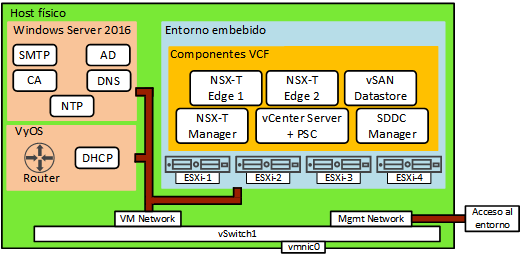
\includegraphics[width=0.6\textwidth]{imaxes/pruebaconcepto/hostFisico.png}
      \caption{Muestra la estructura generada por el instalador VLC. Cuatro hosts ESXi embebidos con los componentes de VMware Cloud Foundation cuyo tráfico circula a través del \textit{port group} VM Network.}
      \label{fig:estructura-generada-por-VLC}
    \end{figure}
    \begin{figure}[h]
      \centering
      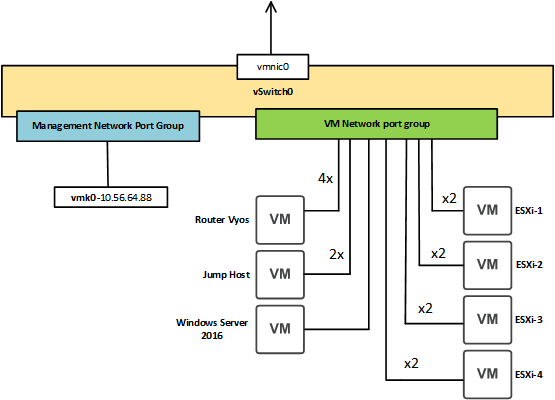
\includegraphics[width=0.6\textwidth]{imaxes/pruebaconcepto/vSwitch0HostFisico.png}
      \caption{Muestra las VMs que están funcionando sobre el host físico y que representan los componentes de la infraestructura física de un SDDC real, junto con el número de interfaces que se utilizan en cada una. Cada host ESXi generado por VLC cuenta con dos interfaces de red. El router VyOS, Jump Host y Windows Server 2016 se configuran antes del despliegue de VMware Cloud Foundation con VLC y se comunican con el entorno generado por VLC a través del \textit{port group} VM Network. El \textit{port group} Management Network se utiliza para acceder a la configuración del host físico a través de la dirección que se indica. Se utiliza la interfaz vmnic0 del host como salida del tráfico generado por el vSwitch0.}
      \label{fig:VMs-alojadas-host-fisico}
    \end{figure}
    \begin{figure}[h]
      \centering
      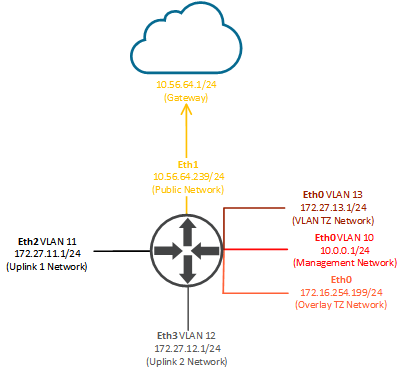
\includegraphics[width=0.4\textwidth]{imaxes/pruebaconcepto/RouterFisicoL3.png}
      \caption{Muestra la configuración del router VyOS. Cada una de las interfaces se debe configurar antes del despliegue de VCF. Todas usan MTU de 8940 Bytes. 
      En las interfaces Eth2 y Eth3 el router utiliza enrutamiento dinámico BGP donde el AS local es 65001 y el AS remoto es AS 65003, configurado para anunciar a sus vecinos la red 10.0.0.0/24 Management Network. Las direcciones configuradas como \textit{neighbour} son: 172.27.11.2, 172.27.11.3, 172.27.12.2 y 172.27.12.3. En la dirección IP 172.27.254.199 de la interfaz eth0, el router proporciona un servidor DHCP que asigna direcciones IP en el rango 172.16.254.0 - 172.16.254.100.}
      \label{fig:interfaces-router-fisico-L3}
    \end{figure}
    \begin{figure}[h]
      \centering
      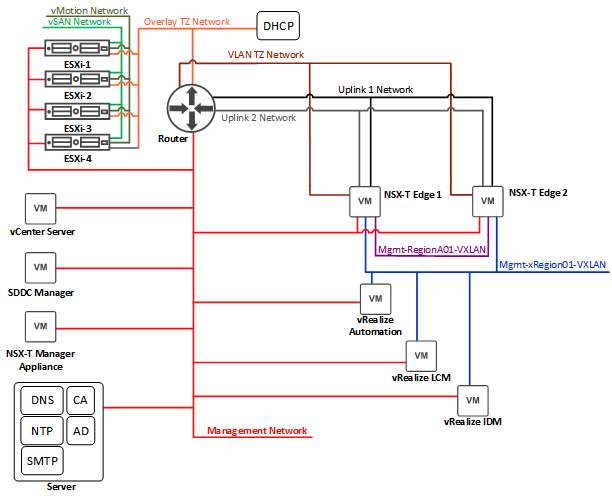
\includegraphics[width=0.6\textwidth]{imaxes/pruebaconcepto/RedDesdeDentro.png}
      \caption{Muestra todos los componentes de VMware Cloud Foundation desplegados por VLC, como se conectan con los distintos servicios de red y a que redes se conectan. Las redes Mgmt-xRegion01-VXLAN y Mgmt-Region01A-VXLAN se corresponden a redes virtuales gestionadas por VMware NSX-T que no requieren ninguna configuración adicional en la capa 3 de la infraestructura física (esto se verá con detalle en el apartado de diseño de VMWare NSX-T).}
      \label{fig:red-L3-infraestructura-fisica}
    \end{figure}
    \FloatBarrier
  \end{subsubsection}
  
\end{subsection}
    %%%%%DISEÑO ARQ. VIRTUAL
\begin{subsection}{Diseño y configuración del Management Domain}
    
    % Esta capa virtual provee infraestructura de almacenamiento, red y cómputo definida por software a través de servicios. En el modelo de despliegue consolidado de VMware Cloud Foundation, todos sus servicios y componentes se encuentran dentro de un mismo cluster (solo una AZ) dentro de la infraestructura, mientras que en el modelo estándar los servicios y componentes de gestión de la infraestructura están situados en clusters distintos (pueden estar en AZ distintas), todos sus componentes se encuentran agrupados en un mismo cluster.
    
    
    
    \subsubsection{Diseño de VMware vCenter Server}
    El componente VMware vCenter Server es el punto de acceso y de control de todas las máquinas virtuales localizados en los hosts ESXi que forman parte de su dominio. En el entorno desplegado se utiliza una instancia de VMware vCenter Server para controlar el \textit{management domain}, se denomina \textit{vcenter-mgmt}. Esta instancia de vCenter Server contiene un dominio que con un cluster vSphere formado por los cuatro hosts ESXi desplegados por VLC, estos se denominan respectivamente \textit{esxi-1}, \textit{esxi-2}, \textit{esxi-3} y \textit{esxi-4}. En vCenter Server se gestionan los recursos de las VMs de cada componente, se monitorizan los recursos, permite la creación y asignación de roles, permisos y usuarios, aisla las redes que usan los recursos que controla de otras instancias de vCenter Server, permite gestionar los grupos de discos de almacenamiento de cada host ESXi que forman el \textit{datastore} de VMware vSAN, administrar las redes a las que se conecta cada componente, en definitiva, VMware vCenter Server es el punto desde el cual se controlan los recursos que utiliza cada componente. Además, incluye el componente PSC que controla el dominio de autenticación de VMware vSphere SSO Domain denominado \textit{local}. Desde vCenter Server también se controlan las características de alta disponibilidad y recuperación ante fallos de VMware vSphere como se verá a continuación. El acceso a vCenter Server se hace a través del componente web vSphere Client.
    \begin{figure}[h]
      \centering
      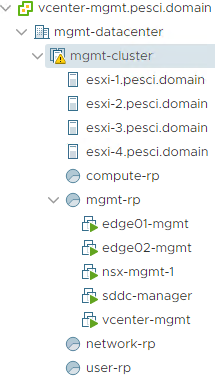
\includegraphics[width=0.2\textwidth]{imaxes/pruebaconcepto/clusterVCenterServer.png}
      \caption{Muestra el dominio (\textit{vcenter-mgmt.pesci.domain} de la instancia de vCenter Server y el cluster vSphere (\textit{mgmt-cluster}) donde se alojan los componentes del \textit{management domain}. Incluye cuatro hosts ESXi y cuatro \textit{resource pools}, uno de ellos contiene las VMs de los componentes dedicados a este \textit{management domain}.}
      \label{fig:cluster-vCenter-Server}
    \end{figure}
    \FloatBarrier
    %  Con vCenter Server se simplifica la escalabilidad del SDDC, la gestión de actualizaciones para los componentes es más sencilla, permite determinar roles específicos y responsabilidades y permite aislar las redes de otras instancias de vCenter Server. Además, para gestionar vSpehere SSO Domain, VMware vCenter Server contiene embebido el componente PSC con todos los servicios necesarios. 
    %  En caso de que existan varios \textit{Workload Domain} se puede habilitar el modo \textit{Enhanced Linked Mode} para poder gestionar todas las instancias de vCenter Server de forma centralizada desde un único vSphere Client.
    % Por lo anterior, en el \textit{management domain} se despliega una instancia de VMware vCenter Server que incluye un cluster de VMware vSphere.
    
    \begin{subsubsection}{Diseño almacenamiento VMware vSAN}
      El almacenamiento del \textit{management domain} desplegado, está implementado con VMwware vSAN. Los cuatro hosts ESXi contienen cuatro grupos de discos cada uno con configuración All-Flash. Como hay cuatro hosts participantes, soporta el fallo de un host lo cual permite dejar hosts fuera de servicio para tareas de mantenimiento. Esto es posible gracias a que con FTT (\textit{Failures-To-Tolerate}) igual a 1 se mantiene la redundancia de los datos almacenados en el \textit{datasotore}, en uno de los hosts. Cada grupo de discos cuenta con cuatro discos uno de ellos para caché, 16 discos en total. Para hacer disponible este servicio de almacenamiento, todos los hosts deben estar conectados a la subred generada para VMware vSAN y utilizar una VLAN para separar su tráfico.
    \end{subsubsection}
        
    \begin{subsubsection}{Diseño cluster VMware vSphere}
    Dentro de un \textit{workload domain} pueden existir varios clusters vSphere con diferentes características según su finalidad. Los hosts ESXi que lo forman pueden ser de diferentes tamaños teniendo en cuenta que se pueden usar menos hosts ESXi de mayor capacidad o más hosts con menores prestaciones, el coste de cada host ESXi, el uso que se le va a dar al cluster y las características máximas y mínimas del cluster vSphere. Para el \textit{management domain} se utiliza un único cluster vSphere con de 4 hosts de los cuales se reserva un host para proveer redundancia. Todos los hosts ESXi cuenta con 64GB de memoria RAM menos uno que tiene 32 GB, y 19.9GHz de CPU. Dentro del cluster hay que configurar los servicios vSphere HA y vSphere DRS para proteger los componentes del SDDC. La configuración que se establece en el \textit{management domain} es la siguiente:
    % En caso de que el \textit{management domain} esté extendido en dos AZ entonces se requieren 4 hosts en cada AZ para proporcionar redundancia y disponibilidad en caso de caída de una de las AZ.
   
    \begin{itemize}
        \item \textbf{vSphere High Availability}: en este servicio la propiedad \textit{Admission Control Policy} permite establecer la cantidad recursos reservados en caso de fallo y como se establece el cálculo de esos recursos. En el \textit{management domain} se configura para el fallo de al menos un host y reserva de recursos según un porcentaje, reservando así el 25\% de la CPU y el 30\% de la memoria RAM ya que funciona mejor cuando las VM usan mucha CPU y memoria. La otra propiedad que se debe habilitar para el correcto funcionamiento del servicio es \textit{VM and Application Monitoring}, que se encarga de reiniciar las VM en caso de caída.
        % que puede ser según el número hosts que pueden fallar en el cluster, según un porcentaje de reserva de rescursos o especificando el host donde se recolocan las VM del host caído.  RAM.  
        \item \textbf{vSphere DRS}: este servicio permite migrar VMs de un host ESXi a otro dentro del mismo cluster vSphere para equilibrar la carga de trabajo y mantener las VMs activas en caso de caída de alguno de los hosts. se activa usando la opción por defecto \textit{Fully Automated} ya que aporta el mejor balance entre consumo de recursos y migraciones de VM innecesarias. Adicionalmente se pueden establecer reglas para determinar reglas de orden de encendido sobre grupos de VM. 
        %En caso de que exista más de una AZ, se deben crear grupos de VM y de hosts de cada AZ para luego implementar reglas de afinidad para que las VM de una AZ no sean migradas a otra AZ ya que esto puede afectar al rendimiento de la VM. 
    \end{itemize}
    % En el modelo consolidado se debe crear un único cluster con un mínimo de cuatro hosts ESXi ya que uno de los hosts se utiliza para asegurar la disponibilidad del almacenamiento vSAN cuando hay algún host inactivo. Este modelo proporciona capacidad de un único fallo por cluster.
    \end{subsubsection}
    \subsubsection{Diseño de red para el cluster vSphere}
    Si bien en VMware Cloud Foundation existe VMware NSX-T, un componente dedicado únicamente a la administración de la red del SDDC, es desde VMware vSphere dónde se encuentran los elementos para establecer redes que separen cada tipo de tráfico de los componentes del SDDC. Estas redes se configuran en base a los siguientes aspectos:
    \begin{itemize}
        \item Separar el tráfico de cada servicio para mejorar la eficiencia de la red y la seguridad. Así se puede ajustar las características de cada red, como el ancho de banda o la latencia, a las necesidades de cada servicio.
        \item Utilizar un único vSphere Distributed Switch por cluster donde se añade un \textit{port groups} por cada servicio.
        % \item Mejorar el rendimiento usando NICs de tipo VMXNET3 en las máquinas virtuales.
        \item Las NICs físicas de cada host ESXi conectados a un mismo vSphere Distributed Switch están conectadas también a la misma red física.
        % \item Aquellas redes que se dedican a servicios de la infraestructura deben estar configuradas con puertos tipo \textit{vmkernel}.
    \end{itemize}
    Para el \textit{management domain} del SDDC se crea un único vSphere Distributed Switch llamado \textit{sddc-vds01} con la siguiente configuración:
    \begin{itemize}
        
        \item Se establece un MTU igual 9000 Bytes para permitir el tráfico de \textit{jumbo frames} ya que son requeridos por algunos de los servicios.
        
        \item Se habilita el servicio \textit{Network I/O} que permite establecer un nivel de prioridad a cada tipo de tráfico. Esto se realiza estableciendo limites de ancho de banda, políticas de balanceo de carga y reserva de recursos para un tipo de tráfico asociado a un servicio. Por cada tipo de tráfico hay cuatro aspectos que se pueden configurar que son \textit{Shares} (indica el \% de ancho de banda que se le da a un tipo de tráfico, el tipo de tráfico que tenga un mayor valor en \textit{Shares} tendrá más prioridad a la hora de usar los recursos), \textit{Reservation} (indica el valor de ancho de banda que se reserva para el tipo de tráfico) y \textit{Limit} (establece un valor máximo para el ancho de banda de un tipo de tráfico). En el \textit{management domain} los tipos de tráfico más relevantes que se deben configurar son los siguientes:
        \begin{itemize}
          \item \textit{Management Traffic}: el valor \textit{Shares} se establece al 50\% (\textit{Normal}) lo cual le da mayor prioridad que el resto de tipos. El resto de valores no se modifican.
          \item \textit{vSphere vMotion Traffic}: el valor \textit{Shares} se establece al 25\% (\textit{Low}) ya que durante el estado normal del entorno este tipo de tráfico no es muy importante. El resto de valores no se modifican.
          \item \textit{vSAN Traffic}: el valor \textit{Shares} se establece al 100\% (\textit{High}) para garantizar que este servicio recibe la cantidad de ancho de banda que necesita. El resto de valores no se modifican.
          \item \textit{Virtual Machine Traffic}: el valor \textit{Shares} se establece al 100\% (\textit{High}) para garantizar que las VMs siempre tienen acceso a la red ya que son una parte importante del SDDC. El resto de valores no se modifican.
        \end{itemize}
        
        \item Para detectar errores de compatibilidad entre la configuración del vSphere Distributed Switch y la red física se habilita el servicio \textit{Health Check}. Este se encarga de comprobar si la configuración de cada VLAN y MTU se adapta a la configuración de la capa física.
        
        \item Como puertos de salida \textit{Uplink} se configuran las interfaces físicas \textit{vmnic0} y \textit{vmnic1}. Como vDS es un componente distribuído, en cada host se usarán ambas interfaces de red como \textit{uplinks}.
        
    \end{itemize}
    En este vSpehere Distributed Switch para el \textit{management domain} se configuran los siguientes \textit{port groups}, que son de tipo \textit{Distributed port group} y de tipo \textit{Uplink port group}:
    \begin{itemize}
           
            \item \textbf{Management port group}: es un \textit{Distributed port group} que comunica a todos los hosts ESXi entre si y transmite el tráfico entre los diferentes componentes de VMware Cloud Foundation, es decir, por este \textit{port group} circulan los comandos de configuración y gestión que los componentes del SDDC se envían entre ellos. Con el nombre \textit{sddc-vds01-mgmt}, en él están configurados los cuatro hosts ESXi y las VMs \textit{vcenter-mgmt}, \textit{sddc-manager}, \textit{nsx-mgmt-1},\textit{edge01-mgmt} y \textit{edge02-mgmt} bajo la subred con IP 10.0.0.0, con máscara de red 255.255.255.0, con VLAN 10 y con MTU igual a 1500 Bytes. Esta red debe ser configurada también en la infraestructura física.
            
            \item \textbf{vMotion port group}: es un \textit{Distributed port group} que está dedicado al tráfico del componente vSphere vMotion para realizar las migraciones de máquinas virtuales de un host a otro. Con el nombre \textit{sddc-vds01-vmotion}, en él están configurados los 4 hosts bajo la subred con IP 10.0.4.0, con máscara de red 255.255.255.0, con VLAN 10 y con MTU igual a 8940 Bytes.
            
            \item \textbf{vSAN port group}: es un \textit{Distributed port group} que está dedicado al servicio de almacenamiento VMware vSAN y por él los hosts acceden al almacenamiento del SDDC. Con el nombre \textit{sddc-vds01-vsan}, en él están configurados los 4 hosts bajo la subred con IP 10.0.8.0, con máscara de red 255.255.255.0, con VLAN 10 y con MTU igual a 8940 Bytes.
            
            \item \textbf{Edge Uplink port group}: es un \textit{Distributed port group} dedicado a las conexiones del component NSX-T Edge que se dedica a dar acceso a determinados servicios y para proporcionar a otros \textit{workload domain} conexión con la red externa. Están gestionados por VMware NSX-T ya que dan servicio a sus componentes. En el entorno existen dos \textit{port groups} para proporcionar redundancia y alta dispobilidad, uno llamado \textit{sddc-edge-uplink01} cuyas instancias están configuradas bajo la red con IP 172.27.11.0 y con máscara de red 255.255.255.0, y otro llamado \textit{sddc-edge-uplink02} cuyas instancias están configuradas bajo la red con IP 172.27.12.0 y máscara de red 255.255.255.0. Ambos \textit{port groups} están configurados como VLAN Trunk (por ellos puede circular tráfico de cualquier VLAN) y tienen un MTU de 8940 Bytes. En los dos están configuradas dos VM llamadas \textit{edge01-mgmt} y \textit{edge02-mgmt}. Estas dos redes también se deben configurar en la infraestructura física.
            
            \item \textbf{Uplink port group}: se trata de un \textit{Uplink port group} al que se le asignan las NICs físicas de cada host para establecer políticas sobre el tráfico que se dirige desde los hosts y VMs hacia fuera del vSphere Distributed Switch. Con el nombre \textit{sddc-vds01-DVUplinks-10}, en él están configuradas las dos NICs físicas de cada host, cada una en una interfaz \textit{uplink}.
            
    \end{itemize}
    \begin{figure}[h]
      \centering
      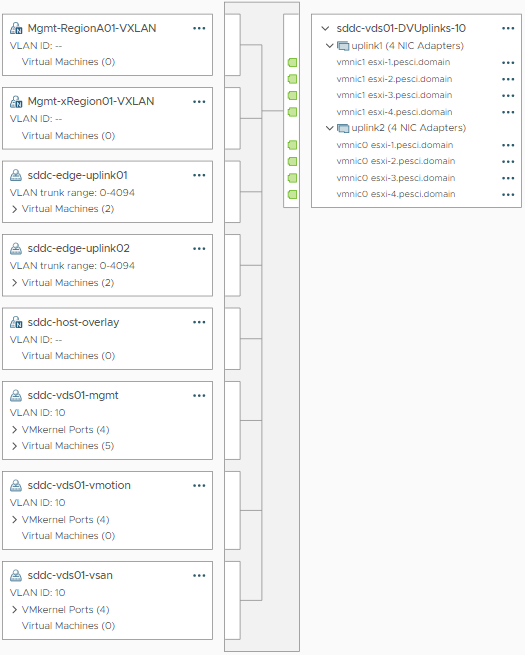
\includegraphics[width=0.4\textwidth]{imaxes/pruebaconcepto/distributedSwitchEntornoFinal.png}
      \caption{Muestra todos los \textit{Distributed Port Groups} y \textit{Uplink port group} que se alojan en el vSphere Distributed Switch (\textit{sddc-vds01}) dedicado al \textit{management domain}. En el \textit{port group} \textit{sddc-vds01-DVUplinks-10} se muestra como a cada interfaz \textit{uplink} se mapea una interfaz física (vmnic) de cada host ESXi. Los \textit{port groups} \textit{mgmt-Region01A-VXLAN}, \textit{mgmt-xRegion01-VXLAN} y \textit{sddc-host-overlay} son generados y administrados por el componente VMware NSX-T como se explicará más adelante. Cada \textit{port group} informa de cuantas VMs y hosts ESXi tiene conectados.}
      \label{fig:port-groups-vSwitch-vSphere}
    \end{figure}
    \FloatBarrier
    La configuración que se aplica a cada \textit{Distributed port group} descrito anteriormente es la siguiente:
    \begin{itemize}
      \item \textit{Port binding}: permite indidcar como se gestionan los puertos de un \textit{port group} cuando se añade o elimina una VM. Tiene dos opciones de configuración, la primera se denomina \textit{Static Port Binding} y su función consiste en asignar un puerto dentro del \textit{port group} a la VM que se conecta y solo se elimina cuando la VM es borrada. La segunda opción se denomina \textit{Ephemeral Port Binding} y consiste en que el puerto se asigna a la VM cuando esta se enciende y se elimina cuando se apaga o elimina. Para los \textit{port groups} \textit{sddc-vds01-vsan} y \textit{sddc-vds01-vmotion} se configura la opción \textit{Static Port Binding} ya que así se asegura que las VMs se conectan siempre al mismo puerto lo cual permite mantener datos históricos y hacer monitoreo a nivel de puerto. Para los \textit{port group} \textit{sddc-vds01-mgmt}, \textit{sddc-edge-uplink01} y \textit{sddc-edge-uplink02} se configura la opción \textit{Ephemeral Port Binding} ya que como el tráfico que circula por ellos es el que gestiona todos los componentes y da acceso a otras redes etonces se elimina la dependencia del estado de vCenter Server permitiendo que la comunicación continúe aunque vCenter Server no se encuentre operativo.
    
      \item \textit{Load Balancing}: indica como se distribuye el tráfico de salida de cada VM/host que se encuentran en el \textit{port group} entre las NICs físicas. Se selecciona \textit{Route based on physical NIC load}, es decir, el tráfico de una VM se transmite por una única NIC por lo que si esa NIC física está saturada, se asignará otra NIC física a la VM.
      
      \item \textit{Network failure detection}: esta opción permite establecer como debe determinar el \textit{port group} que alguna de las NICs físicas está fuera de servicio. Se selecciona \textit{Link status only} para que esto se determine según el estado que le transmite la NIC física, así se pueden detectar los fallos que ocurren en la red física.
      
      \item \textit{Notify switches}: se habilita para permitir a los host enviar \textit{frames} a los switches físicos para que estos conozcan la localización de las VM que están funcionando en cada host.
      
      \item \textit{Failback}: permite determinar como se reactiva una NIC cuando esta se recupera de un fallo. Se habilita para establecer que la NIC se marcará como activa inmediatamente después de que se haya recuperado. Esta opción se debería desactivar en caso de que el estado de la NIC sea inestable.
      
      \item \textit{Failover Order}: permite determinar que uplinks se deben utilizar, los que se seleccionan como \textit{active} son los que se utilizarán por defecto, los que se seleccionan como \textit{stand by} se usarán cuando los uplinks marcados como \textit{active} se encuentren desactivados. Se seleccionan las dos interfaces \textit{uplink} disponibles en el estado \textit{active}. Para el \textit{port group} \textit{sddc-edge-uplink01} se selecciona la interfaz \textit{uplink1} como activa y se deja sin usar la interfaz \textit{uplink2}, mientras que se configura de forma contraria en el \textit{port group} \textit{sddc-edge-uplink02}.
    \end{itemize}
    
    
    %%%%%%%%%%%%%%%%%%%%%%%%%%%%%%%%%%%%%%%%%%%%
    \subsubsection{Diseño de la red del SDDC con VMware NSX-T}
    En un SDDC debe existir una red virtual, es decir, definida por software o también conocida como \textit{Software-Defined Network}. Esta red al estar construída con componentes de software, se desacopla de la red física sobre la que funciona lo que hace posible que se pueda modificar sin necesidad de cambiar la configuración en la capa física, reduciendo así la complejidad de la red física y el tiempo dedicado a la gestión de la misma. Además, este tipo de arquitectura habilita la posibilidad de implementar múltiples configuraciones de red en tiempo reducido proporcionando elasticidad y flexibilidad a la hora de administrar los recursos, tanto para el administrador como para el usuario final.
    El componente encargado de crear, configurar y administrar la red virtualizada del SDDC es VMware NSX-T que a su vez contiene otros componentes entre los que se dividen distintas responsabilidades y funciones, ya descritos anteriormente.
    
    %%%%% 1 - EXPLICACION DE LOS COMPONENTES DE NSX Y LOS QUE HAY EN EL ENTORNO
    %%%%% 2 - COMO SE DEBE CONFIGURAR LA CAPA FÍSICA Y COMO ESTÁ IMPLEMENTADA EN EL ENTORNO ( parte de esto ya está definido en la parte de red física, REVISAR) => Meter la descripción de lo físico con el resto (modificar ese apartado) [https://docs.vmware.com/en/VMware-Validated-Design/6.0/sddc-architecture-and-design-for-the-management-domain/GUID-C924E896-D9C4-47BF-91D5-DF72605EF63E.html]
    %%%%% 3 - REDES QUE HAY Y COMO SE EXTIENDEN ENTRE AZs
    %%%%% 4 - COMO FUNCIONAN LAS COMUNICACIONES (GENEVE, ROUTING ...)
    
    % En esta sección se describe como VMware Cloud Foundation abstrae la red física en un conjunto de recursos virtuales de red, utilizando los servicios de VMware NSX para crear una capa virtual independiente de la infraestructura física.
    Aunque se recomienda desplegar tres instancias de NSX-T Manager en el \textit{management domain}, VLC solo despliega una única instancia llamada \textit{nsx-mgmt-1} para mejorar el rendimiento del entorno. Además, VLC también genera dos instancias de NSX-T Edge que se denominan \textit{edge01-mgmt} y \textit{edge02-mgmt}. %cada conjunto de instancias de cada componente forman un cluster donde cada VM está protegida por las funcionalidades vSphere HA y vSphere DRS para proveer alta disponibilidad del servicio y migrar las VMs a otra ubicación en caso de caída de una AZ o de un host. 
    Estas VMs están conectadas al \textit{port group} \textit{sddc-vds01-mgmt} que les permite comunicarse entre ellas y con vCenter Server, además las instancias de NSX-T Edge también están conectadas a otros dos \textit{Distributed port group} llamados \textit{sddc-edge-uplink01} y \textit{sddc-edge-uplink02}. %Si existe más de una AZ, varios de los \textit{distributed port groups} se deben extender al resto de AZs para que en caso de que la primera AZ falle sus VMs se puedan migrar a otra AZ y sigan teniendo conectividad. Los \textit{port groups} que deberían estar extendidos en todas las AZ son el \textit{port group} \textit{sddc-vds01-mgmt} de cada AZ\footnote{Cada AZ tiene su propio \textit{Management port group}, entonces en cada AZ debe ser accesible el \textit{Management port group} del resto de AZs.}, los \textit{port group} \textit{sddc-edge-uplink01}, \textit{sddc-edge-uplink02} y \textit{port group} \textit{Edge Overlay}.
    
    Los elementos que utiliza VMware NSX-T para crear una red independiente de la configuración de la red física son \textit{Segment} y \textit{Transport Zone}. Con estos componentes VMware NSX-T puede crear túneles que definen redes de capa 2 sin necesidad de realizar ningún cambio en la configuración de la red física.
    \begin{itemize}
      \item \textbf{Transport Zone} (TZ): define el alcance de la red virtual. Pueden ser de dos tipos distintos, basada en VLAN o basada en Overlay. Una TZ se puede asignar a varios TN que tendrán acceso a los \textit{segments} que funcionen en esa TZ. Un TN se conecta a una TZ a través de un N-VDS los cuales pueden pueden estar conectados a varias TZ de tipo VLAN pero solo a una TZ de tipo Overlay al mismo tiempo.
      
      \item \textbf{Segment}: también llamado \textit{Logical Switch}, representa un dominio de broadcast de capa 2 que forma parte de una \textit{Transport Zone}. El tipo de tráfico puede ser VLAN u Overlay dependiendo de como se haya configurado la \textit{Transport Zone} de la que forma parte. Las VMs de cada TN se pueden conectar a los \textit{Segments} situados en las \textit{Transport Zones} a las que el host está conectado. Estas VMs se pueden comunicar con el resto de VMs conectadas al mismo \textit{Segment}.
       
    \end{itemize}
    Para gestionar las conexiones de cada TN, tanto para los nodos NSX-T Edge como para los hosts ESXi, VMware NSX-T introduce el componente llamado \textbf{NSX-T Virtual Distributed Switch} (N-VDS). Cada TN del \textit{management domain} posee un N-VDS, este elemento conecta sus interfaces a los \textit{segments} que se configuran en cada TN. Para el \textit{management domain} del entorno, VLC despliega dos \textit{transport zones} diferentes.
    \begin{figure}[h]
      \centering
      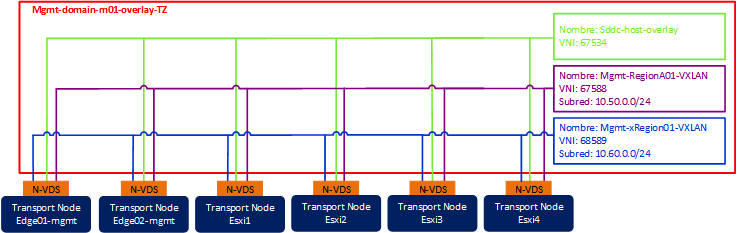
\includegraphics[width=1\textwidth]{imaxes/pruebaconcepto/OverlayTZSegments.png}
      \caption{Se muestra la \textit{transport zone} con el nombre \textit{mgmt-domain-m01-overlay-tz} de tipo Overlay. Está extendida en los seis TNs que hay en el \textit{management domain} y contiene tres \textit{segments}. El \textit{segment} \textit{mgmt-xRegion01-VXLAN} se utiliza para desplegar aplicaciones que deben ser accesibles desde todas las \textit{regions} que existan en el SDDC, es decir, la misma instancia de una aplicación está disponible desde varios puntos, así se reduce el consumo de recursos y aumenta la disponibilidad de esas aplicaciones ya que pueden migrar a distintas localizaciones según el estado de los recursos. El \textit{segment} \textit{mgmt-Region01A-VXLAN} tiene como finalidad alojar aplicaciones solo deben ser accesibles desde dentro de una misma \textit{region}. En estos dos \textit{segments} es donde se colocan los productos de VMware vRealize. Por último, el \textit{segment} \textit{sddc-host-overlay} es utilizado por los componentes de VMware NSX-T para comunicarse con y entre los diferentes TNs. VMware NSX-T genera en el vSphere vSwitch un \textit{port group} por cada \textit{segment} para poder conectar la VM de cada componente al \textit{port group} que le corresponda.}
      \label{fig:overlay-TZ-segments-NSXT}
    \end{figure}

    \begin{figure}[h]
      \centering
      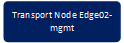
\includegraphics[width=1\textwidth]{imaxes/pruebaconcepto/VLANTZSegments.png}
       \caption{Muestra la\textit{transport zone} con el nombre \textit{sfo01-m01-edge-uplink-tz} de tipo VLAN. Está extendida en los dos TNs \textit{edge01-mgmt} y \textit{edge02-mgmt} y contiene dos \textit{segments}. Ambos \textit{segments} \textit{VCF-edge-mgmt-cluster-segment-11} y \textit{VCF-edge-mgmt-cluster-segment-12} son utilizados por las instancias de NSX-T Edge para transmitir el tráfico que proviene de los \textit{segments} donde se despliegan aplicaciones hacia la red externa (esto se explicará con más detalle). Estos \textit{segments} utilizan los \textit{port groups} \textit{trunk} del vSphere Switch para transmitir su tráfico hacia las interfaces de red físicas de cada host.}
      \label{fig:VLAN-TZ-segments-NSXT}
    \end{figure}

    \FloatBarrier
    %\begin{itemize}
      % \item \textit{mgmt-domain-m01-overlay-tz}:
      %   \begin{itemize}
      %     \item Tipo: Overlay
      %     \item Transport Nodes: \textit{edge01-mgmt}, \textit{edge02-mgmt}, \textit{esxi1}, \textit{esxi2}, \textit{esxi3} y \textit{esxi4}.
      %     \item Segments:
      %       \begin{itemize}
      %         \item \textit{mgmt-xRegion01-VXLAN}:
      %           \begin{itemize}
      %             \item VNI: 68589
      %             \item Subred: 10.60.0.0/24
      %             \item VMs: \textit{vrlcm} (10.60.0.60), \textit{vridm} (10.60.0.30)
      %             \item Descripción: se usa para desplegar las aplicaciones (algunos productos de VMware vRealize Suite lo utilizan) que deben ser accesibles desde todas las \textit{Regions} del SDDC, por lo tanto este \textit{segment} debe estar extendido en todo el entorno para que las VMs que se alojen en él puedan mantener la misma configuración de red independientemente del lugar físico donde se encuentren.
      %           \end{itemize}
      %         \item \textit{mgmt-Region01A-VXLAN}:
      %           \begin{itemize}
      %             \item VNI: 67588
      %             \item Subred: 10.50.0.0/24
      %             \item Descripción: su finalidad es alojar aplicaciones que sean accesibles desde una misma \textit{Region}. El alcance de estas aplicaciones está limitado a una \textit{Region} por lo tanto este \textit{segment} solo está extendido dentro de la misma.
      %           \end{itemize}
      %         \item \textit{sddc-host-overlay}:
      %           \begin{itemize}
      %             \item VNI: 67534
      %             \item Descripción: \textit{segment} usado por los componentes de VMware NSX-T para comunicarse entre los diferentes hosts ESXi.
      %           \end{itemize}
      %       \end{itemize}
      %   \end{itemize}
    %   \item \textit{sfo01-m01-edge-uplink-tz}:
    %     \begin{itemize}
    %       \item Tipo: VLAN
    %       \item Transport Nodes: \textit{edge01-mgmt} y \textit{edge02-mgmt}.
    %       \item Segments:
    %         \begin{itemize}
              
    %           \item \textit{VCF-edge-mgmt-cluster-segment-11}:
    %             \begin{itemize}
    %               \item VLAN: 11
    %               \item VMs: \textit{edge01-mgmt} (172.27.11.2/24) y \textit{edge02-mgmt} (172.27.11.3/24).
    %               \item Descripción: usado para transmitir el tráfico saliente hacia la red física.
    %             \end{itemize}
    %           \item \textit{VCF-edge-mgmt-cluster-segment-12}:
    %             \begin{itemize}
    %               \item VLAN: 12
    %               \item VMs: \textit{edge01-mgmt} (172.27.12.2/24) y \textit{edge02-mgmt} (172.27.12.3/24).
    %               \item Descripción: usado para transmitir el tráfico saliente hacia la red física.
    %             \end{itemize}
    %         \end{itemize}
    %       \end{itemize}
    % \end{itemize}
    
    Las TZ, tanto las basadas en Overlay como las basadas en VLAN, sirven para comunicar TNs que se encuentran en distintas partes de la infraestructura física (por ejemplo, en distintos racks) como si estuvieran situadas en el mismo dominio broadcast de capa 2 físico. 
    Aquellas que usan Overlay utilizan el protocolo Geneve para crear un túnel entre los puntos de origen y destino por el cual circula el tráfico generado por los \textit{segments} que pertenecen a esa TZ y que debe salir a la red física para alcanzar su destino. El protocolo Geneve añade una cabecera UDP a cada paquete Ethernet que generan los \textit{segments} cuando este sale del TN donde se generó hacia un TN situado en otra red física. La nueva cabecera incorpora un identificador llamado VNI y es único para cada \textit{segment} (cada \textit{segment} tiene su propio identificador VNI). 
    \begin{figure}[h]
      \centering
      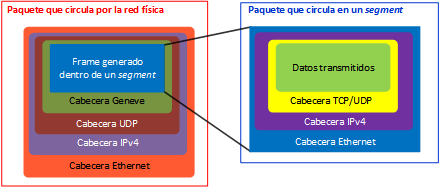
\includegraphics[width=1\textwidth]{imaxes/pruebaconcepto/FrameGeneve.png}
      \caption{Muestra las cabeceras que forman un paquete de red que pertenece a un \textit{segment} cuando este sale de un TN. Cuando el paquete que circula por la red virtual (contiene los datos que se transmiten y la información de las VMs origen y destino) tiene salir a la infraestructura física para alcanzar el destino, el \textit{transport node} añade la cabecera del protocolo Geneve con el identificador VNI correspondiente, una cabecera UDP con un puerto origen y destino establecidos por defecto, una cabecera IP con las direcciones IP origen y destino de los TN que se están comunicando, y una cabecera Ethernet donde se idican las direcciones MAC de los TN origen y destino. Así, dos VMs conectadas al mismo \textit{segment} pero alojadas en TNs de dominios broadcast diferentes, pueden comunicarse de forma transparente como si estuvieran conectadas directamente una con la otra en la misma subred.}
      \label{fig:Frame-Geneve-Segment-NSXT}
    \end{figure}
    \FloatBarrier
    % \begin{figure}[h]
    %   \centering
    %   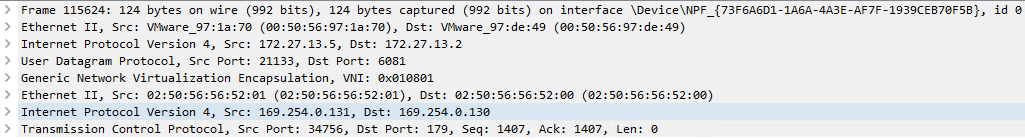
\includegraphics[width=1\textwidth]{imaxes/pruebaconcepto/FrameExampleGeneve.png}
    %   \caption{Cabeceras de un paquete capturado con el programa Wireshark que utiliza encapsulación Overlay. Contiene un VNI, las direcciones IP de los elementos que se comunican dentro del \textit{segment} y las direcciones IP de los TN que se comunican \textit{}}
    %   \label{fig:Frame-Geneve-Example-NSXT}
    % \end{figure}
    En las TZ de tipo VLAN, tráfico de sus \textit{segments} es encapsulado añadiendo un identificador de VLAN definido en una plantilla \textit{Uplink Policy}\footnote{A las TZ de tipo Overlay no se les aplica ninguna \textit{Uplink Policy}.} que se asigna a la TZ. Se aplica la misma VLAN para encapsular el tráfico de todos los \textit{segments} de una misma TZ de tipo VLAN. Estas plantillas permiten establecer como debe el N-VDS de un TN tratar el tráfico de la \textit{transport zone} a la que se asigna. En cada una se especifican varias \textit{Teaming Policy}, la VLAN que debe usar el N-VDS cuando tiene que enviar el tráfico fuera del TN y el MTU de cada interfaz \textit{uplinks}. Una \textit{Teaming Policy} indica como el N-VDS utiliza los \textit{uplinks} a nivel de \textit{segment} para distribuir el tráfico y conseguir conexiones redundantes y balanceo de la carga, se especifica una \textit{Teaming Policy} por defecto más otras adicionales. Se aplica una \textit{Uplink Policy} a la TZ de tipo VLAN  \textit{sfo01-m01-dge-uplink-tz}.
    %***UPLINKPOLICY**%
    %  Además, en una \textit{Uplink Policy} se define un mapeo con las interfaces \textit{uplink} establecidas en vSphere Distributed Switch (uplink1 y uplink2) para dirigir el tráfico de cada TZ hacia la red física. 
    %Los TNs \textit{edge01-mgmt} y \textit{edge02-mgmt} proporcionan acceso a la red externa a los \textit{segments} de VMware NSX-T, por ello requieren estar conctados a los dos tienen sus interfaces conectadas a los \textit{uplinks} están mapeados con las NICs físicas de cada host ESXi a través de  a los que están ancladas ambas VMs, es decir, un \textit{uplink} está mapeado con una NIC física del host ESXi. 
    %En las TZ de tipo VLAN, se utilizan plantillas .
    \begin{figure}[h]
      \centering
      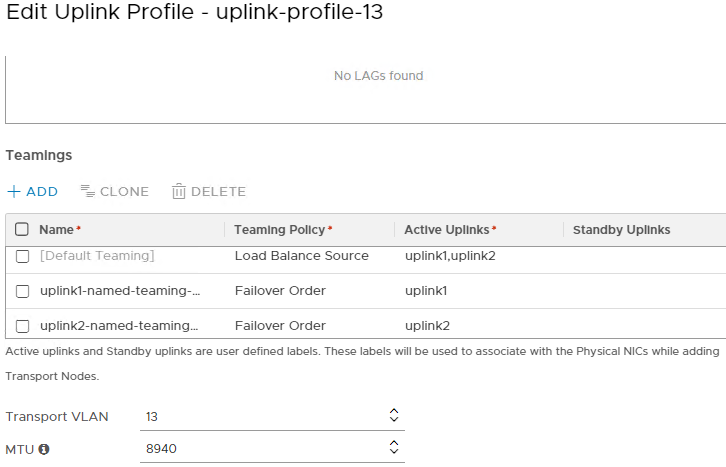
\includegraphics[width=1\textwidth]{imaxes/pruebaconcepto/UplinkPolicy13.png}
      \caption{Muestra la \textit{Uplink Policy} (\textit{uplink-profile-13}) configurada para la TZ \textit{sfo01-m01-dge-uplink-tz}. Se establece la VLAN 13 como Transport VLAN, utilizado para encapsular el tráfico saliente hacia la red física, y MTU de 8940 Bytes para los uplinks. Hay definidas tres \textit{Teaming Policies}, una por defecto (\textit{Default teaming}) que utiliza \textit{Load Balance Source} para hacer un mapeo uno a uno entre las interfaces de cada VM y uno de los \textit{uplinks} (todo el tráfico correspondiente a esa interfaz se envía y recibe por el mismo \textit{uplink}), y dos adicionales \textit{uplink1-named-teaming-policy} y \textit{uplink2-named-teaming-policy} que utilizan \textit{Failover Order} donde se establece un \textit{uplink} como activo por donde se transmite todo el tráfico y otros de reserva que se usan en caso de que el \textit{uplink} activo falle (en una de las políticas todo el tráfico se reenvía por \textit{uplink1} y en la otra por \textit{uplink2}).}
      \label{fig:Uplink-Policy-13-NSXT} 
    \end{figure}
    \FloatBarrier
    A los \textit{segments} \textit{VCF-edge-mgmt-cluster-segment-11} y \textit{VCF-edge-mgmt-cluster-segment-12} pertenecientes a la TZ \textit{sfo01-m01-dge-uplink-tz} se les asigna la \textit{Teaming Policy} \textit{uplink1-named-teaming-policy} y \textit{uplink2-named-teaming-policy} respectivamente. De esta forma se consigue que el tráfico que circula por cada uno de ellos solo utilice un único \textit{uplink}. 
    \begin{figure}[h]
      \centering
      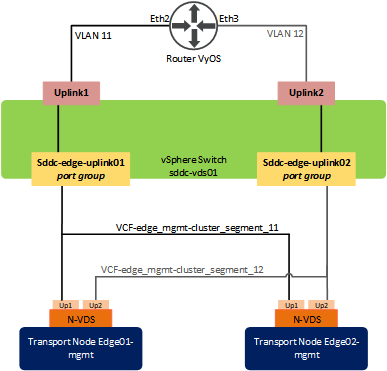
\includegraphics[width=0.6\textwidth]{imaxes/pruebaconcepto/UplinkDesign.png}
      \caption{Muestra la topología que forman las instancias de NSX-T Edge para generar la redundancia y alta disponibilidad en las rutas hacia la red externa para las aplicaciones cuya red está gestionada por VMware NSX-T, desde el punto de vista de VMware vSphere. Cada TN Edge posee dos interfaces \textit{uplink} que durante su configuración se mapea cada una con uno de los \textit{trunk port groups} de vSphere Switch. Las interfaces \textit{uplink} que se indican en la \textit{Teaming Policy} se refieren a las de la instancia de NSX-T Edge, no las de vSphere vSwitch, por lo tanto cada uno de los \textit{segments} utiliza solo uno de los \textit{uplinks} que combinado con la configuración de los \textit{port groups} de vSphere vSwitch establecen las rutas que se muestran en la imagen.}
      \label{fig:Uplink-Design-Edge-NSXT} 
    \end{figure}
    \FloatBarrier
    % Así, como cada TN de NSX-T Edge está anclado a dos \textit{trunk port groups} en vSphere Switch por donde se transmite el tráfico de estos dos \textit{segments} y cada uno de esos \textit{segments} transmite por un único \textit{uplink}, se consigue que estas rutas hacia la red externa sean redundantes y con alta disponibilidad para las aplicaciones cuya red está gestionada por VMware NSX-T.
    % Para la TZ de tipo VLAN \textit{sfo01-m01-dge-uplink-tz} se especifica la siguiente \textit{Uplink Policy}:
    % \begin{itemize}
    %   \item Nombre: \textit{uplink-profile-13}
    %   \item Transport VLAN: 13
    %   \item MTU: 8940
    %   \item Teaming Policy: se especifican tres, una por defecto y dos adicionales:
    %     \begin{itemize}
    %       \item \textit{Default teaming}: \textit{Load Balance Source}, hace un mapeo uno a uno entre cada interfaz virtual de cada VM y uno de los \textit{uplinks} del N-VDS, así todo el tráfico correspondiente a esa interfaz se envía y recibe por el mismo \textit{uplink}.
          
    %       \item \textit{uplink1-named-teaming-policy}: \textit{Failover Order}, se establece un \textit{uplink}, \textit{uplink1} en este caso, como activo que se utiliza para enviar todo el tráfico, y una lista de \textit{uplinks} ordenados que se utilizan en caso de que el primero no esté disponible, vacía para esta \textit{Teaming policy}.
    %       \item \textit{uplink2-named-teaming-policy}: \textit{Failover Order}, donde el \textit{uplink} activo es \textit{uplink2} y la lista de \textit{uplinks} de reserva está vacía.
    %     \end{itemize}
    % \end{itemize}
    % A los \textit{segments} de esta TZ, \textit{VCF-edge-mgmt-cluster-segment-11} y \textit{VCF-edge-mgmt-cluster-segment-12} se les asignan las \textit{Teaming Policy} \textit{uplink1-named-teaming-policy} y \textit{uplink2-named-teaming-policy} respectivamente. Con esta configuración el tráfico de cada \textit{segment} circula por una única NIC física del host ESXi. Esto, junto con la configuración \textit{Failover Order} establecida para los \textit{port groups} \textit{sddc-edge-uplink01} y \textit{sddc-edge-uplink02} en el vSphere vDS,se consigue que el tráfico de salida hacia la red física perteneciente a los componentes de VMware NSX-T y todas las aplicaciones cuya red gestiona VMware NSX-T, sea distribuído por dos redes distintas proporcionando redundancia y disponibilidad del servicio en caso de que ocurra una caída de alguna de las conexiones.
    %*****************%

    Esta encapsulación, tanto VLAN como Overlay, tiene lugar cuando los paquetes salen de la interfaz de una VM y entran en el N-VDS del TN. Para ello, cada TN tiene dispositivo llamado \textit{Tunnel End Point} (TEP) al que se le asigna una dirección IP utilizada para enviar y recibir el tráfico entre VMs que se encuentran en el mismo \textit{segment} pero se alojan en TNs situados en redes L2 diferentes\footnote{En el entorno desplegado todos los TN se encuentran dentro de la misma red física. Esto implica que no se genere tráfico con los TEPs ya que todas las TZs funcionan sobre un único dominio broadcast.}. Los TNs que son hosts ESXi obtienen su dirección TEP de un servidor DHCP\footnote{El servidor DHCP hace que se simplifique el proceso de configuración de un nuevo host ESXi ya que le asigna una dirección IP de forma automática.} mientras que los que son instancias de NSX-T Edge la dirección IP se asigna de forma manual. El TEP de cada TN tiene dos direcciones IP asignadas puesto que cada uno tiene dos interfaces de red, \textit{esxi-1} tiene las direcciones 172.16.254.10 y 172.16.254.11, \textit{esxi-2} tiene las direcciones 172.16.254.12 y 172.16.254.13, \textit{esxi-3} tiene las direcciones 172.16.254.14 y 172.16.254.15, \textit{esxi-4} tiene las direcciones 172.16.254.16 y 172.16.254.17, \textit{edge01-mgmt} tiene las direcciones 172.27.13.2 y 172.27.13.3, y \textit{edge02-mgmt} tiene las direcciones 172.27.13.4 y 172.27.13.5.
    
    Al crear un \textit{segment} dentro de una TZ, se configura un modo de replicación que indica como se retransmite el tráfico Broadcast, Multicast y Unknown Unicast propio del \textit{segment} cuando este tiene que viajar a un TN que está en una ubicación distinta en el medio físico. El modo de replicación que se utiliza en todos los \textit{segments} es \textit{Two-Tier Hierarchical Mode}. 
    \begin{figure}[h]
      \centering
      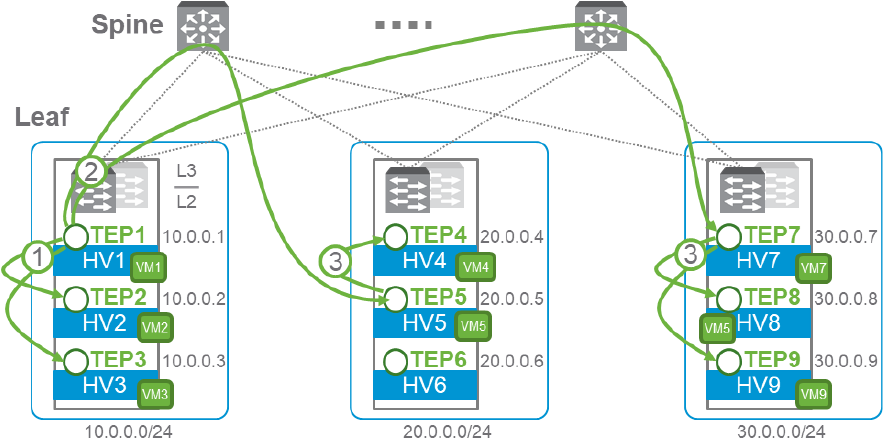
\includegraphics[width=0.6\textwidth]{imaxes/pruebaconcepto/Two-tier-ReplicationMode.png}
      \caption{Ejemplo de como funciona el modo de replicación \textit{Two-Tier Hierarchical}. (1) Cuando el TN HV1 envía tráfico BUM a la red primero lo hace a los TNs que están en su mismo dominio, (2) después envía una copia de ese tráfico a un único TN de cada dominio broadcast donde exista el \textit{segment} propietario del tráfico y, finalmente, (3) el TN de cada localización lo retransmite al resto de TNs de su dominio que lo requieran. De este modo se reduce el número de paquetes que el TN origen debe enviar a través de la red física.}
      \label{fig:Frame-Geneve-Segment-NSXT}
    \end{figure}
    \FloatBarrier
    % Este consiste en que cuando desde un TN se envía algún tipo de tráfico BUM de un \textit{segment} cuyos TNs están distribuídos en distintos puntos de la infraestructura física, el TEP del TN origen detecta que debe retransmitir el tráfico a una red externa, en la red externa se selecciona un TN que recibe el tráfico y lo reenvía al resto de TNs dentro del mismo dominio de red que deben recibir ese tráfico, así se reduce . El tráfico solo se enviará a los TN que contienen VMs que forman parte del \textit{segment} que lo genera. Es el componente NSX-T Controller quien se encarga de actualizar e indicar a los TNs toda la información para que esta comunicación sea correcta.
    
    El objetivo es crear nuevas subredes, es decir \textit{segments} que se expanden por los distintos TNs adheridos a la \textit{transport zone} correspondiente, y conectarlas a un router virtual para al final formar subredes distribuidas con servicios de red también	distribuidos y virtualizados, todo gestionado desde VMware NSX-T y sin tener que configurar la red física. Para completar esto, VMware NSX-T introduce routers virtuales que se encuentran embebidos y distribuídos dentro del hypervisor ESXi de cada TN y que proporcionan enrutamiento entre \textit{segments} y servicios de red distribuídos. Permiten definir un \textit{gateway} para cada \textit{segment} a través del cual las VMs conectadas pueden acceder a la red externa y los servicios de red. La herramienta VLC despliega para el \textit{management domain} un modelo de enrutamiento de doble capa (\textit{Two Tier Routing}) donde se utilizan dos routers virtuales, \textit{Tier-0} (\textit{mgmt-domain-tier0-gateway}) dedicado a gestionar el acceso a la red externa a través del router VyOS con conexiones redundantes, y \textit{Tier-1} (\textit{mgmt-domain-tier1-gateway})que gestiona el enrutamiento entre \textit{segments} y proporciona servicios de red a las VMs.

    \begin{figure}[h]
      \centering
      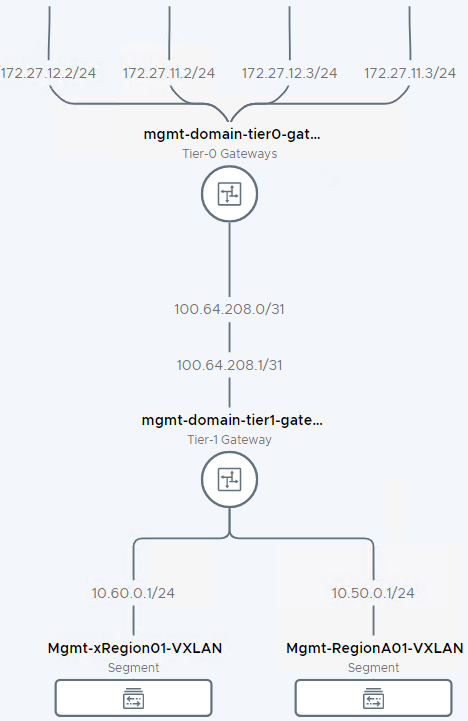
\includegraphics[width=0.5\textwidth]{imaxes/pruebaconcepto/topologiaTwoTierRouting.png}
      \caption{Muestra la topología del modelo de dos routers virtuales y los \textit{segments} a los que se conecta cada uno desde el punto de vista de NSX-T. El router de Tier-1 enruta el tráfico entre los \textit{segments} a los que está conectado y hacia el router de Tier-0 que se encarga de transmitir el tráfico hacia la red física.}
      \label{fig:Topology-TwoTier-Routing-NSXT}
    \end{figure}
    \FloatBarrier
    Un router router lógico está formado por dos componentes:
    \begin{itemize}
      
      \item \textbf{Distributed Router} (DR): que gestiona el enrutamiento y se a subredes a través de sus interfaces lógicas. Estas subredes pueden ser \textit{segments} u otro DR. A cada interfaz se le asigna una dirección MAC y una dirección IP que representa el \textit{gateway} de la subred. Este componente está distribuído en todos los TN, tanto hosts ESXi como instancias de NSX-T Edge manteniendo la misma configuración (interfaces,tablas de enrutamiento, etc.). Su función es redirigir el tráfico que recibe entre las interfaces que tiene disponibles, es decir, enruta el tráfico entre los diferentes \textit{segments} a los que está conectado el router virtual Tiene una interfaz llamada \textit{Internal transit Link} conectada a la red \textit{Internal Transit Network} que se utiliza para conectar todos los DR y SR de un \text{Tier} distribuídos en los TN.
      
      \item \textbf{Service Router} (SR): proporciona servicios de red de forma centralizada (NAT, DHCP, Load Balancer, VPN, Gateway Firewall y Bridging L2) y proporciona acceso a la red externa. Este componente no está distribuído entre los diferentes TN, solo se se encuentra distribuido en las instancias de NSX-T Edge. Los servicios que proporciona solo se entregan a los recursos cuya red está gestionada por VMware NSX-T. Posee la interfaz \text{Internal Transit Link} para comunicarse con el resto de DR y SR pertenecientes al mismo \text{Tier}, dos interfaces \textit{External Interface} que se conectan a los \text{segments} que dan acceso a la red externa \footnote{La \textit{External Interface} solo existe en \textit{Tier-0} ya que es el router que se comunica con el dispositivo físico.}, la interfaz \textit{Router Link}\footnote{Router Link Network utiliza por defecto la subred 100.64.0.0/16.} que conecta el SR de \textit{Tier-0} con el de \textit{Tier-1}, y la interfaz \textit{Internal transit} que se habilita cuando se activa la opción \textit{Inter SR iBGP}\footnote{Inter SR iBGP Network utiliza por defecto la subred 169.254.0.0/24.} y que comunica los SR de las dos instancias de NSX-T Edge.
    \end{itemize}

    \begin{figure}[h]
      \centering
      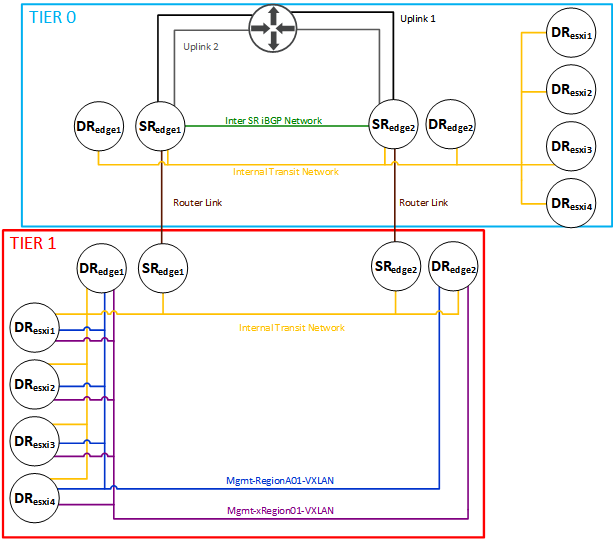
\includegraphics[width=0.8\textwidth]{imaxes/pruebaconcepto/EstructuraInternaTiers.png}
      \caption{Muestra los componentes internos de cada router virtual y como estos están distribuidos por todos los TNs. El router \textit{mgmt-domain-tier0-gateway} tiene el componente SR distribuído en dos TN que son las instancias de NSX-T Edge, y el componente DR distribuido en todos los TNs. El SR situado en \textit{edge01-mgmt} está conectado al \textit{segment} \textit{VCF-edge\_mgmt-edge-cluster-segment-11} y usa la dirección IP 172.27.11.2, y otra interfaz conectada al \textit{segment} \textit{VCF-edge\_mgmt-edge-cluster-segment-12} donde usa la IP 172.27.12.2, mientras que el SR de \textit{Tier-0} situado en \textit{edge02-mgmt} se conecta a los mismos \textit{segments} pero usando las direcciones 172.27.11.3 y 172.27.12.3 respectivamente. El router \textit{mgmt-domain-tier1-gateway} tiene el componente SR distribuido en las dos instancias de NSX-T Edge y el componente DR distribuido por en todos los TNs. Ambos SR están conectados con los SR de \textit{Tier-0} para transmitir el tráfico hacia la red física. Los DR de \textit{Tier-1} están conectados a los \textit{segments} \textit{Mgmt-RegionA01-VXLAN} y \textit{Mgmt-xRegion01-VXLAN} para proporcionar enrutamiento y servicios a las VMs situadas en ellos.}
      \label{fig:estructura-interna-TwoTier-Routing-NSXT}
    \end{figure}
    \FloatBarrier
    
    La razón de tener dos capas de enrutamiento se debe a la configuración del router \textit{mgmt-domain-tier0-gateway}. En este router se utiliza BGP para comunicarse con el router físico a través de las \textit{external interfaces} (se establece 65003 como \textit{autonomous system} local)\footnote{El uso de BGP simplifica la configuración de nuevas rutas cuando se añaden componentes al entorno, y que no se pierda la conectividad en caso de caída de alguna de las interfaces. Este protocolo también se configura en las interfaces del router Vyos}, la opción \textit{Inter SR iBGP} establecer una comunicación mediante BGP entre las instancias distribuídas del componente SR de \textit{Tier-0} para que se pueda seguir transmitiendo el tráfico en caso de que alguna de las interfaces de una instancia de NSX-T Edge esté fuera de servicio, se activa el protocolo ECMP para balancear el tráfico hacia la red física entre los caminos disponibles ya que en conjunto, en el router de \textit{Tier-0} existen cuatro rutas posibles para alcanzar el router VyOS. Un aspecto importante es la configuración de la disponibilidad de un router virtual ya que determina el modo en el que se va a ejecutar. En el router de \textit{Tier-0} se selecciona el modo \textit{active-active} el cual implica que las dos instancias de SR funcionan ambas de forma activa, es decir, el tráfico que reciba cada una será encaminado por una subred diferente proporcionando así mayor ancho de banda, mayor disponibilidad y mayor escalabilidad. Esto esto último no es compatible con servicios de red centralizados, por ello es necesario desplegar al menos un router lógico de \textit{Tier-1} (\textit{mgmt-domain-tier1-gateway}) configurado con el modo \textit{active-stanby} el cual solo se utiliza una de las dos instancias del SR de \textit{Tier-1} por lo tanto el tráfico dirigido a este router siempre será recogido en un único punto. Así, en el router \textit{mgmt-domain-tier1-gateway} es donde se pueden desplegar servicios de red como NAT, Load Blancing, DNS y VPN, para los \textit{segments} que están conectados.
    % Las interfaces de cada router lógico son de los siguientes tipos:
    
    % \begin{itemize}
    %   \item \textit{External Interface}: se refiere a las interfaces que conectan con el dispositivo de la red física, normalmente un router.
    %   \item \textit{Internal Transit Link}: está interfaz conecta a todos los DR de \textit{Tier-0} distribuídos en cada TN con los SR formando una única red.
    %   \item \textit{RouterLink Interface}: interfaz que conecta un router lógico de \textit{Tier-1} con uno de \textit{Tier-0} a través de una subred generada por defecto (100.64.0.0/16).
    % \end{itemize}
    
    % Los routers lógicos creados para el \textit{management domain} en el entorno tienen la siguiente configuración:
    
    % \begin{itemize}
    %   \item \textbf{mgmt-domain-tier0-gateway}: su función consiste en proporcionar acceso a la red física.
    %     \begin{itemize}
    %       \item \textit{External Interfaces}\footnote{Estas direcciones corresponden a las interfaces de los TN NSX-T Edge que conectan con las interfaces Uplink sobre dos \textit{segments} de tipo VLAN.}: Dos que se conectan al \textit{segment} \textit{VCF-edge\_mgmt-edge-cluster-segment-11} (172.27.11.2 y 172.27.11.3) y dos que se conectan al \textit{segment} \textit{VCF-edge\_mgmt-edge-cluster-segment-12} (172.27.12.2 y 172.27.12.3).
    %       \item \textit{Internal Transit Link}: Usa la subred 169.254.0.0/24.
    %       \item \textit{RouterLink Interface}: Tiene la dirección 100.64.192.0/31.
    %       \item Configuración: se 
    %       \item Configuración HA: determina el modo en el que se va a ejecutar el router de \textit{Tier-0}. En este caso se selecciona el modo \textit{active-active} el cual implica que las instancias de SR (una en cada nodo NSX-T Edge) funcionan ambas de forma activa, el tráfico que reciba cada una será encaminado por una subred diferente. Es por esto que el router lógico de \textit{Tier-0} no puede ofrecer servicios centralizados.
    %     \end{itemize}
    
    %   \item \textbf{mgmt-domain-tier1-gateway}: router de \textit{Tier-1} dedicado a gestionar el enrutamiento de las VMs de aplcaciones no dedicadas a la administración del SDDC. 
    %   \begin{itemize}
    %     \item \textit{Internal Transit Link}: Usa la subred 164.254.0.0/24.
    %     \item \textit{RouterLink Interface}: Tiene la dirección 100.64.192.1/31.
    %     \item \textit{Segment Interfaces}: conectado al \textit{segment} \textit{mgmt-Region01A-VXLAN} con la dirección IP 10.50.0.1, y al \textit{segment} \textit{mgmt-xRegion01-VXLAN} con la dirección IP 10.60.0.1.
    %     \item Configuración HA: determina el modo en el que se va a ejecutar el router de \textit{Tier-1}. En este caso se selecciona el modo \textit{active-stanby} el cual solo utiliza una de las dos instancias del SR de \textit{Tier-1} (cada una en un nodo de NSX-T Edge) por lo tanto el tráfico que reciba solo será encaminado por un único punto. Esto permite activar servicios centralizados, por lo tanto será \textit{mgmt-domain-tier1-gateway} y no \textit{mgmt-domain-tier0-gateway} el encargado de proporcionarlos.
    %   \end{itemize}
    % \end{itemize}
    
    % Así como el componente DR de los routers de \textit{Tier-0} y de \textit{Tier-1} están distribuídos por todos los TNs (incluídas las instancias de NSX-T Edge), el componente SR solo se encuentra en las VMs de NSX-T Edge por lo tanto son estas VMs las que proporcionan los servicios centralizados de SR y acceso a la red externa del entorno. Además, para que los componentes lógicos tengan acceso a los \textit{segments} descritos, las instancias de NSX-T Edge están conectadas a dos TZs:
    % \begin{itemize}
      
    %   \item \textit{mgmt-domain-m01-overlay-tz}: esta TZ proporciona a las VMs del entorno a los servicios de los routers de \textit{Tier-0} y de \textit{Tier-1} y también permite que esos routers lógicos tengan acceso a los \textit{segments} donde se encuentran esas VMs. Se utiliza el tipo Overlay para que se puedan comunicar TNs que se encuentran en distintas redes físicas sin que la configuración de la red física sea compleja.
      
    %   \item \textit{sfo01-m01-dge-uplink-tz}: esta TZ se utiliza para conectarse a la red física a través de un router físico. Se utiliza el tipo VLAN para encapsular el tráfico saliente hacia al router físico y porque las VLANs usadas en los \textit{segments} dentro de esta TZ se configuran también en la infraestructura física, por lo tanto no hace falta crear una capa física virtual con Overlay.
    % \end{itemize}
    
    % Para gestionar las conexiones de cada TN, tanto para los nodos NSX-T Edge como para los hosts ESXi, VMware NSX-T introduce el componente llamado \textbf{NSX-T Virtual Distributed Switch} (N-VDS). Cada TN del entorno posee un N-VDS, este elemento conecta sus interfaces a los \textit{segments} que se configuran en cada TN y establece un mapeo con las interfaces \textit{uplink} que se utilizan para dirigir el tráfico de cada TZ hacia el exterior del TN. En el caso de las instancias de NSX-T Edge, los dos \textit{uplinks} están mapeados con las NICs físicas de cada host ESXi a través de los dos \textit{distributed port groups} de vSphere vDS (\textit{sddc-edge-uplink01} y \textit{sddc-edge-uplink02}) a los que están ancladas ambas VMs, es decir, un \textit{uplink} está mapeado con una NIC física del host ESXi. 
    % En las TZ de tipo VLAN, se utilizan plantillas \textit{Uplink Policy} para indicar como debe el N-VDS tratar el tráfico de la \textit{transport zone} a la que se asigna. En cada \textit{Uplink Policy} se especifican varias \textit{Teaming Policy}, el identificador VLAN que debe usar el N-VDS cuando tiene que enviar el tráfico fuera del TN y el MTU de los \textit{uplinks}. Una \textit{Teaming Policy} indica como el N-VDS utiliza los \textit{uplinks} para conseguir conexiones redundantes y balanceo de la carga, en una \textit{Uplink Policy} se especifica una \textit{Teaming Policy} por defecto y otras adicionales.
    % Para la TZ de tipo VLAN \textit{sfo01-m01-dge-uplink-tz} se especifica la siguiente \textit{Uplink Policy}:
    % \begin{itemize}
    %   \item Nombre: \textit{uplink-profile-13}
    %   \item Transport VLAN: 13
    %   \item MTU: 8940
    %   \item Teaming Policy: se especifican tres, una por defecto y dos adicionales:
    %     \begin{itemize}
    %       \item \textit{Default teaming}: \textit{Load Balance Source}, hace un mapeo uno a uno entre cada interfaz virtual de cada VM y uno de los \textit{uplinks} del N-VDS, así todo el tráfico correspondiente a esa interfaz se envía y recibe por el mismo \textit{uplink}.
          
    %       \item \textit{uplink1-named-teaming-policy}: \textit{Failover Order}, se establece un \textit{uplink}, \textit{uplink1} en este caso, como activo que se utiliza para enviar todo el tráfico, y una lista de \textit{uplinks} ordenados que se utilizan en caso de que el primero no esté disponible, vacía para esta \textit{Teaming policy}.
    %       \item \textit{uplink2-named-teaming-policy}: \textit{Failover Order}, donde el \textit{uplink} activo es \textit{uplink2} y la lista de \textit{uplinks} de reserva está vacía.
    %     \end{itemize}
    % \end{itemize}
    % A los \textit{segments} de esta TZ, \textit{VCF-edge-mgmt-cluster-segment-11} y \textit{VCF-edge-mgmt-cluster-segment-12} se les asignan las \textit{Teaming Policy} \textit{uplink1-named-teaming-policy} y \textit{uplink2-named-teaming-policy} respectivamente. Con esta configuración el tráfico de cada \textit{segment} circula por una única NIC física del host ESXi. Esto, junto con la configuración \textit{Failover Order} establecida para los \textit{port groups} \textit{sddc-edge-uplink01} y \textit{sddc-edge-uplink02} en el vSphere vDS,se consigue que el tráfico de salida hacia la red física perteneciente a los componentes de VMware NSX-T y todas las aplicaciones cuya red gestiona VMware NSX-T, sea distribuído por dos redes distintas proporcionando redundancia y disponibilidad del servicio en caso de que ocurra una caída de alguna de las conexiones.
    
    
    
    % Estas conexiones están gestionadas por un N-VDS dentro de cada instancia. Este switch lógico utiliza tres interfaces que se conectan a las diferentes redes lógicas. Para aquellas redes lógicas que requieren salida al medio físico ya sea para comunicarse con otros TN o para acceder a la red externa, el N-VDS utiliza finalmente el switch VDS de VMware vSphere que conecta con las interfaces físicas del host ESXi donde corre la instancia de NSX-T Edge.
    
    % la utilizan tres interfaces para  Estas interfaces son \textit{eth0} que se dedica a la red \textit{Management}, \textit{fp-eth0} y \textit{fp-eth1} que ambas se dedican a la conexión con cada uno de los \textit{segments} Uplink. 
    
    
    % *********************************************
    
    %%%%%%%%
    % Se recomienda que la red física siga una topología de tipo \textit{Leaf-Spine} donde existen swithces que se conectan a los hosts (\textit{leaf switches}), que a su vez se conectan a otra capa de switches (\textit{spine switches}) que finalmente conecta con la red principal del SDDC. Este tipo de topología permite medir mejor su rendimiento y facilita la escalabilidad de la infraestructura. En caso de existir varias AZ, debe existir una red física entre ellas cuya capa 3 funcione con enrutamiento dinámico para automatizar la resolución de problemas en caso de caída de alguna de las conexiones.
    %%%%%%%%%
    
    % \iffalse
    % La información sobre VTEP existentes, la relación entre direcciones MAC de máquinas virtuales y dirección IP de VTEP, y relación entre direcciones MAC de máquinas virtuales y su IP, la poseen las instancias de NSX Controller en tres tablas: 
    %     \begin{itemize}
    %         \item \textit{VTEP Table}, relación entre un VTEP y la VXLAN que tiene acceso: VNI (ID del segmento), IP (dirección IP del VTEP), Segment (dirección IP del segmento), MAC (dirección MAC de la NIC física donde está configurado el VTEP).
    %         \item \textit{MAC Table}, relación entre la dirección MAC de una máquina virtual y el VTEP que le da acceso: VNI (ID del segmento), MAC (dirección MAC de la máquina virtual accesible por la VTEP-IP), VTEP-IP (dirección IP del VTEP que da acceso a la máquina virtual de la MAC indicada).
    %         \item \textit{ARP Table}, relación entre la dirección MAC y la dirección IP de una máquina virtual: VNI (ID del segmento), IP (dirección IP de la máquina virtual), MAC (dirección MAC de la máquina virtual).
    %     \end{itemize}
    % Estas tablas permiten reducir la cantidad de tráfico en la red ya que las máquinas virtuales y dispositivos de enrutamiento ya no requieren enviar tráfico Broadcast para obtenerla.
    % La comunicación directa entre máquinas virtuales situadas en distintos hosts ESXi se realiza con tráfico Unicast entre sus respectivos VTEP, pero una máquina virtual también puede enviar tráfico dirigido a todas las máquinas virtuales que pertenecen a su mismo Logical Switch, es decir, a las máquinas de la misma \textit{trasnport zone}, pero pueden situarse en segmentos de red físicos distintos. Este tipo de tráfico puede ser Multicast, Unknown Unicast y Broadcast (BUM), y en VMware NSX se puede gestionar con tres modos de replicación distintos\footnote{Al configurar un Logical Switch se elige uno de los modos.}, modo Multicast, modo Unicast y modo Híbrido.
    %     \begin{itemize}
    %         \item \textbf{Modo Multicast}: requiere que en la red física se haya configurado una IP multicast para cada VXLAN (es decir, Logical Switch), y el protocolo IGMP Snooping en los switches físicos para crear grupos multicast y que el tráfico sea más eficiente, esto habilita multicast entre los VTEP de la misma subred que el emisor. Para transmitir este tráfico a VTEPs situados en otros segmentos de red, se debe configurar el protocolo PIM para poder enrutarlo con los dispositivos de capa 3 físicos. Esta configuración no permite desacoplar la red lógica de la red física.\\
    %         Se puede establecer un grupo multicast por cada VXLAN, esto implica que un host solo recibirá tráfico si tiene al menos una máquina virtual en el grupo, pero requiere configurar muchos grupos. Otra opción es crear un grupo multicast para todas las VXLAN, se necesitan menos direcciones IP pero se genera más tráfico en la red.
    %     \begin{figure}[h!]
    %     \centering
    %     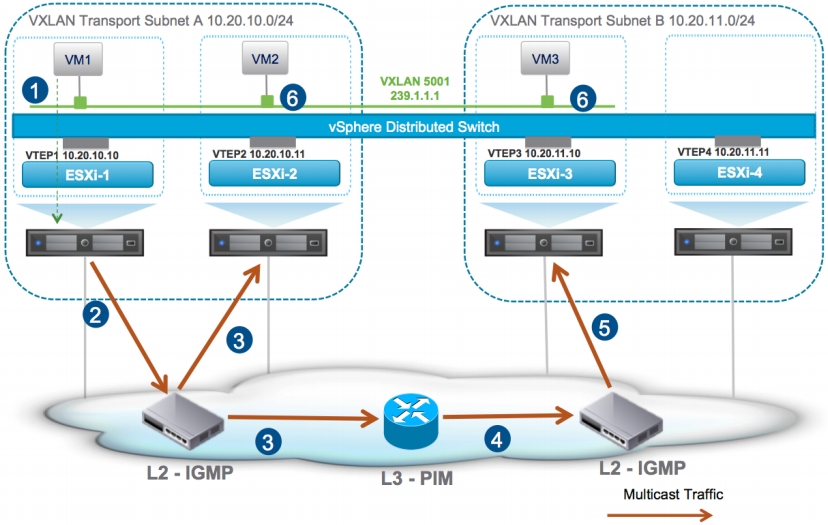
\includegraphics[width=0.5\textwidth]{imaxes/conceptosPrevios/MulticastSeqBUM.png}  \caption{Replicación del tráfico BUM en el modo Multicast}
    %     \label{fig:modoMulticast}
    %     \end{figure}
    %     \FloatBarrier
    %         \item \textbf{Modo Unicast}: no requiere ninguna configuración específica en la capa física y está gestionado por VMware NSX. Se crea un grupo con los VTEP situados en el mismo segmento de red, dentro de cada grupo se selecciona un host ESXi para el rol de \textit{Unicast Tunnel End Point} (UTEP), encargado de recibir el tráfico BUM que procede de otros segmentos de red para reenviarlo por su segmento pero solo a los hosts con al menos una máquina virtual. El host ESXi emisor utiliza la tabla VTEP para comprobar que VTEPs están situados en una VXLAN y así poder dirigir el tráfico BUM correspondiente.\\
    %         Este modo es útil en entornos pequeños donde no hay mucho tráfico y cada segmento de red tiene pocos VTEP.
    %     \begin{figure}[h!]
    %     \centering
    %     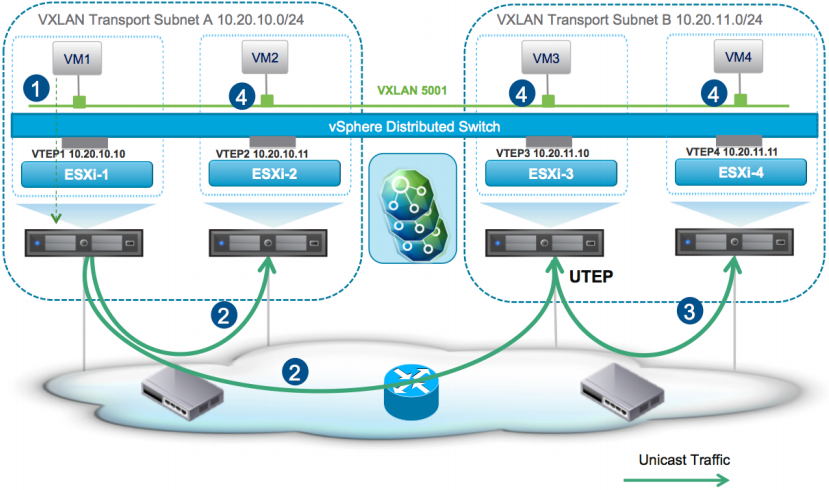
\includegraphics[width=0.5\textwidth]{imaxes/conceptosPrevios/UnicastMode.png}
    %     \caption{Replicación del tráfico BUM en el modo Unicast}
    %     \label{fig:modoUnicast}
    %     \end{figure}
    %     \FloatBarrier
    %         \item \textbf{Modo Híbrido}: combina el modo Unicast y el modo Multicast. El tráfico dirigido a las máquinas virtuales situadas en el mismo segmento de red se transmite usando Multicast, por lo que se requiere tener el protocolo IGMP configurado en los dispositivos físicos de capa 2, se recomienda establecer una dirección Multicast por cada VXLAN. El tráfico se replica a los hosts ESXi que forman parte del grupo. Cuando el tráfico va dirigido a máquinas virtuales situadas en hosts en distinto segmento de red, se transmite utilizando Unicast, como en ese modo, se forma un grupo con los hosts de cada segmento y de cada grupo se elige un host con el rol de \textit{Multicast Tunnel EndPoint} (MTEP). Así, el host que origina el tráfico BUM lo transmite al MTEP correspondiente, el cual se encarga de replicar ese tráfico por su segmento de red. La replicación del tráfico entre segmentos es gestionada por las instancias de NSX Controller.\\
    %         Este modo de replicación permite desplegar NSX en entornos grandes gracias a que el tráfico Multicast y Unicast se pueden escalar facilmente, el primero se reduce a cada segmento de red y la transmisión del segundo en la capa 3 está gestionado por VMware NSX sin necesidad de configurar los dispositivos físicos.
    %     \begin{figure}[h!]
    %         \centering
    %         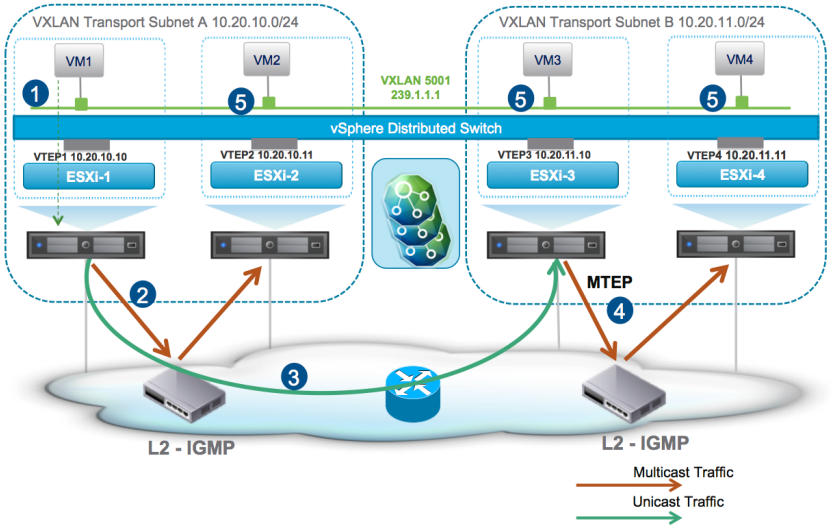
\includegraphics[width=0.5\textwidth]{imaxes/conceptosPrevios/hibrydMode.png}
    %         \caption{Replicación del tráfico BUM en el modo Híbrido}
    %         \label{fig:modoHibrido}
    %     \end{figure}
    %     \FloatBarrier
    %     \end{itemize}
    
    %  El enrutamiento del tráfico está gestionado por dos componentes Distributed Logical Router (DLR) y NSX Edge Services Gateway (ESG). Un mismo DLR se extiende por varios hosts ESXi para enrutar el tráfico entre VXLANs, también mantiene una conexión con las instancias de ESG para transmitir el tráfico que se dirige a redes externas, esa conexión se denomina \textit{transit network} y está getionada por un Logical Switch. Cada DLR tiene su propio Logical Router Control para intercambiar las rutas disponibles con las instancias de ESG, posteriormente, son las instancias de NSX Controller las que transmiten esta información al DLR distribuido en los hosts ESXi. Las interfaces lógicas del DLR conectan con cada Logical Switch, cada interfaz tiene una dirección IP que representa el \textit{gateway} del segmento de red al que esté conectada [Fig. \ref{fig:logicalRoutingCompo} y \ref{fig:redLogicaOne}]. Estos dispositivos utilizan enrutamiento dinámico (protocolos OSPF o BGP).
     
    %  \begin{figure}[h!]
    %   \centering
    %   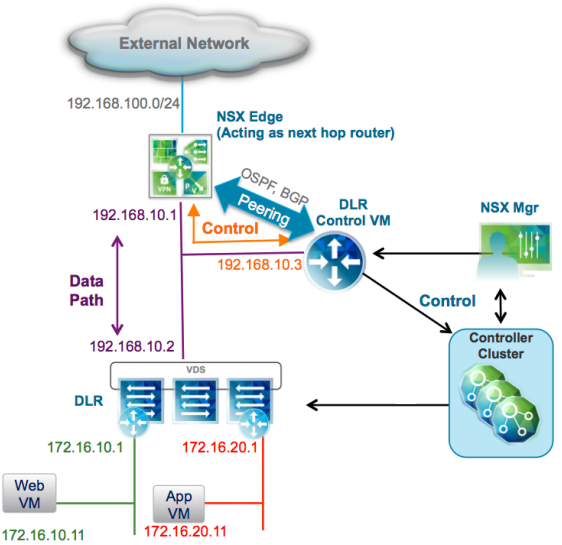
\includegraphics[width=0.4\textwidth]{imaxes/conceptosPrevios/LogicalRoutingComponents.png}
    %   \caption{Componentes de la red virtual que intervienen en el enrutamiento del tráfico.}
    %   \label{fig:logicalRoutingCompo}
    % \end{figure}
    % \FloatBarrier
    
    % \begin{figure}[h!]
    %   \centering
    %   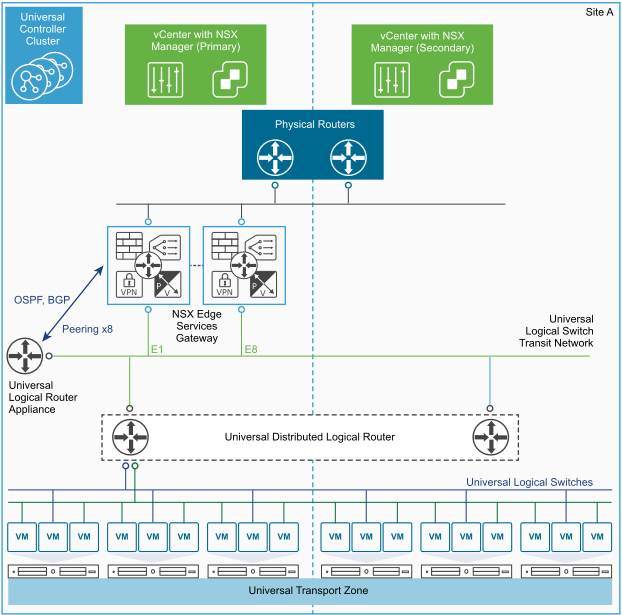
\includegraphics[width=0.5\textwidth]{imaxes/conceptosPrevios/redlogCF.png}
    %   \caption{Red lógica formada en un SDDC con dos clusters.}
    %   \label{fig:redLogicaOne}
    % \end{figure}
    % \FloatBarrier
     
    %  En el SDDC deben existir, al menos, dos intancias de ESG aunque se pueden desplegar hasta 8 instancias. En el modelo consolidado se debe tener un único UDLR para que las rutas entre hosts ESXi sean más cortas, debe existir un Logical Switch que forme la \textit{transit zone}. En el modelo estándar debe existir un UDLR extendido por todos los \textit{Management Cluster} (si hay varias \textit{Regions}), un UDLR extendido por el \textit{Shared Edge and Compute Cluster} y el resto de \textit{Compute Clusters} en cada \textit{Region}, y un DLR extendido por todos los clusters de una misma región.En el modelo estándar existen dos tipos de \textit{transit zones}, una entre el UDLR que atraviesa todas las \textit{Regions} y cada instancia de ESG, y otra que conecta el DLR propio de cada \textit{Region} y sus instancias de ESG. 
    % \\
    % Algunos componentes de VMware Cloud Foundation se deben desplegar en una VXLAN dedicada para proporcionar recuperación ante fallos en caso de que parte del SDDC deje de funcionar. Entre otros componentes (solo vamos a tratar aquellos que son obligatorios), VMware vRealize Log Insight se debe desplegar en una red de este tipo, llamada \textit{Application Virtual Network} (AVN). En entornos con varias \textit{Regions} se crea una \textit{transport zone} que se extiende por todo el SDDC y una \textit{transport zone} adicional en cada \textit{Region}, la primera proporciona recuperación ante fallos a través de todo el SDDC a los componentes que lo requieran, y la segunda solo a través de una \textit{Region}, sin necesidad de reconfigurar direcciones IP o DNS. VMware vRealize Log Insight se debe desplegar en una VXLAN por cada \textit{Region}.
    % \\
    % El acceso a una AVN se realiza a través de las instancias de ESG desplegadas en el entorno, estas se conectan a un UDLR que gestiona el tráfico de la s máquinas virtuales que tiene conectadas. El enrutamiento debe ser dinámico con BGP y las instancias de ESG proporcionan protegen y balacean la carga de trabajo con los servicios de VMware NSX Firewall y Load Balancing [Fig. \ref{fig:avnConsolidated}].\\
    % **VERIFICAR LO DEL LOAD BALANCING en el despliegue. ¿solo para las que son cross-region o tambien en las de una sola region**\\
    % \begin{figure}[h!]
    %   \centering
    %   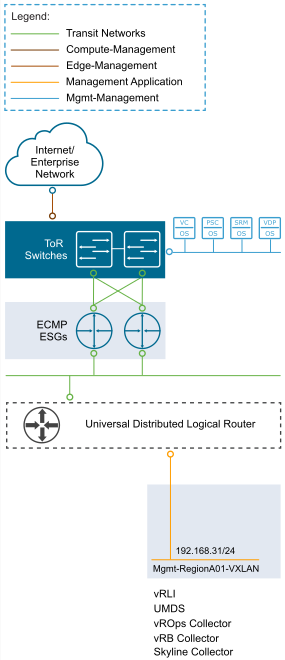
\includegraphics[width=0.25\textwidth]{imaxes/conceptosPrevios/AVNConsolidated.png}
    %   \caption{AVN en el modelo consolidado}
    %   \label{fig:avnConsolidated}
    % \end{figure}
    % \FloatBarrier
    
    % Este utiliza los componentes vCenter Server, NSX Manager, NSX Controllers y NSX Logical Switch para establecer comunicaciones y aislar los distintos tipos de tráfico [Fig. \ref{fig:planosNSX}]. Estos componentes \underline{actúan en diferentes planos} de la red:
    
    
    
    % \begin{itemize}
    %     \item \textbf{Plano de Datos}: esta capa gestiona la transmisión del tráfico entre los componentes del SDDC. En este plano actúan NSX Logical Switches segregando los tipos de datos, y el enrutamiento y firewall distribuído de NSX. Se transmite a través de una red física dedicada al transporte.
    %     \item \textbf{Plano de Control}: aquí se gestionan los mensajes de control que se usan para la configuración de los dispositivos de NSX como switches, routers y firewalls en cada host ESXi. Se distribuye en redes físicas de forma segura usando VLANs para aislarlo del plano de datos.
    %     \item \textbf{Plano de gestión}: aquí se gestiona el tráfico dedicado a la administración de los recursos como puede ser la creación y eliminación de máquinas virtuales. Está controlado por vCenter Server y NSX Manager.
    % \end{itemize}
    % \begin{figure}[h!]
    %   \centering
    %   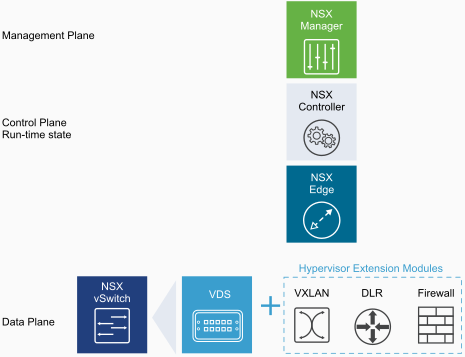
\includegraphics[width=0.65\textwidth]{imaxes/conceptosPrevios/planosNSX.png}
    %   \caption{Como se estructuran las componentes de VMware NSX for vSphere}
    %   \label{fig:planosNSX}
    % \end{figure}
    % \FloatBarrier
    
    %\fi
    
    % \iffalse
    % \subsubsection{Almacenamiento Virtual}
    % VMware vSAN forma único \textit{datastore} con todos los dispositivos de almacenamiento que se encuentran en la infraestructura permitiendo establecer políticas y gestionar esos recursos de forma más simple. Para que funcione correctamente es necesario \underline{configurar una red para VMware vSAN} teniendo en cuenta los siguientes aspectos:
    % \begin{itemize}
    %     \item El uso de vSpehere Distributed Switches genera mejor rendimiento.
    %     \item Se recomienda el uso de paquetes tipo \textit{jumbo frames}.
    %     \item Asignar una VLAN al tráfico de cada cluster de VMware vSAN.
    %     \item Si se implementa en un SDDC con dos localizaciones, es necesario establecer un host \textit{witness}.
    % \end{itemize}
    % Al establecer el tamaño y capacidad de este cluster hay que tener en cuenta que cuantos más hosts ESXi se incluyan, mayor tolerancia a fallos se tendrá y mejor se podrán repartir los grupos de discos entre todos los hosts. Debe haber un balance entre el hardware y la capacidad requerida.
    
    
    % \fi
    \end{subsection}
    
    
    \begin{subsection}{Operaciones de la Arquitectura\cite{CFopermanagement}}
    En este apartado se define como se gestionan en VMware Cloud Foundation las tareas de administración de todas las partes de la infraestructura. Estas tareas se agrupan en la gestión del ciclo de vida y la recopilación de información sobre el estado de cada componente existente.
    
    \subsubsection{Gestión del Ciclo de Vida}
    Elementos que se encargan de administrar el ciclo de vida de los componentes:
    \begin{itemize}
    %     \item \textbf{vSphere Update Manager}: por cada instancia de VMware vCenter Server se despliega una instancia de vSphere Update Manager. Este componente utiliza el servicio \textit{Update Manager Download Service} (UMDS) para obtener las actualizaciones de la red externa al SDDC, el cual se despliega en una red AVN [Fig. \ref{fig:avnConsolidated}], permitiendo limitar el acceso a Internet de vSphere Update Manager y reduciendo el número de descargas ya que un UMDS se comparte entre varias instancias de VMware vCenter Server. Se crea una instancia de UMDS por cada \textit{region} existente [Fig. \ref{fig:UpdateManagerArc}].
    %     \begin{figure}[h!]
    %         \centering
    %         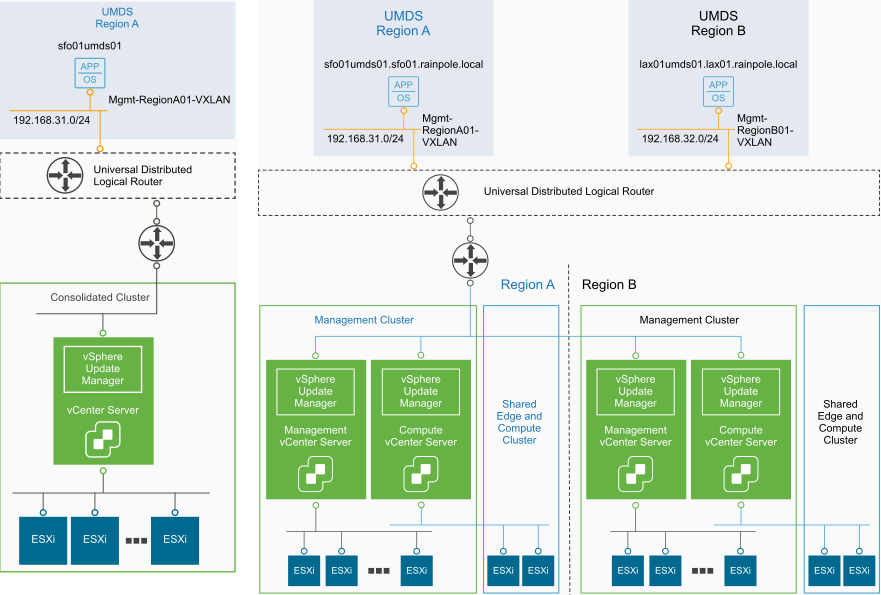
\includegraphics[width=0.5\textwidth]{imaxes/conceptosPrevios/UpdateManagerArch.png}
    %         \caption{Diseño de vSphere Update Manager en el modelo consolidado (izquierda) y en el modelo estándar (derecha)}
    %         \label{fig:UpdateManagerArc}
    %     \end{figure}
    %     \FloatBarrier
        
        \item \textbf{vRealize Suite Licfecycle Manager}: componente utilizado para desplegar, actualizar y configurar, de forma automatizada, los productos vRealize Operations, vRealize Log Insight, vRealize Automation y vRealize Business Cloud. De este componente se despliega una única instancia en una AVN accesible desde cada \textit{region} por todas las instancias de VMware vCenter Server. Se debe registrar su nombre de dominio en el servidor DNS para hacerla accesible.
        
    %     \iffalse
    %     y se puede elegir entre dos modelos de despliegue, uno en el que se usa una máquina virtual denominada  que se encarga de descargar los archivos requeridos por vSphere Update Manager mientras este se encuentra en un entorno aislado [Fig. \ref{fig:updateManager}], y otro donde es la instancia de vSphere Update Manager la que realiza la descarga de los ficheros. La primera opción incrementa la seguridad y permite compartir estos archivos entre distintas instancias de vSphere Update Manager.\\
    %     Una vez desplegado se pueden establecer diferentes configuraciones a nivel de host, máquina virtual y cluster, para que durante la instalación de actualizaciones el servicio del SDDC continúe operativo y evitar la pérdida de información y errores en los recursos.
    %     \begin{figure}[h!]
    %   \centering
    %   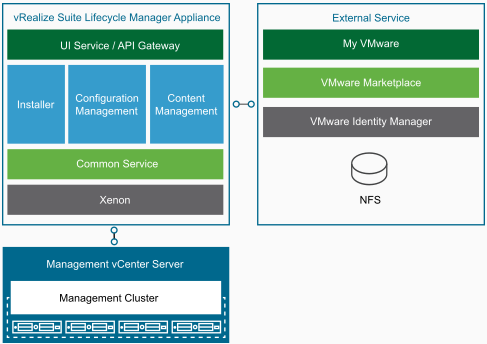
\includegraphics[width=0.8\textwidth]{imaxes/conceptosPrevios/vRealizeUpdateArchLifeCyle.png}
    %   \caption{Estructura de la gestión del ciclo de vida con vRealize Suite Lifecycle Manager.}
    %   \label{fig:vrealizeUpdateManager}
    % \end{figure}
    % \FloatBarrier
    %     \fi
    
    
    \end{itemize}
    
    
    
    
    % \subsubsection{Gestión de Logs}
    % En VMware Cloud Foundation el producto vRealize Log Insight provee gestión y análisis de los logs de la infraestructura. Este componente resgistra los logs, alarmas y eventos de Platform Services Controller, instancias de VMware vCenter Server, de los hosts ESXi, componentes de VMware NSX, vRealize Suite Lifecycle Manager y componentes de vRealize Automation, utilizando el protocolo \textit{syslog} para su obtención. En el modelo consolidado se recomienda desplegar vRealize Log Insight en tamaño reducido, es decir, un solo nodo \textit{master} que gestiona los logs de todos los componentes, pero también se pueden desplegar otros nodos \textit{worker}. Para el modelo estándar se deben desplegar al menos tres nodos por cada \textit{region}, uno \textit{master} y dos \textit{worker}, y el uso de Load Balancer proporciona tolerancia a fallos en caso de que falle uno de los nodos. En ambos modelos los nodos se despliegan en una AVN que solo se extiende por una \textit{region} [Fig. \ref{fig:redLogIsight}], también se deben configurar la dirección IP y nombre de dominio de cada nodo en el servicio DNS.
    %     \begin{figure}[h!]
    %   \centering
    %   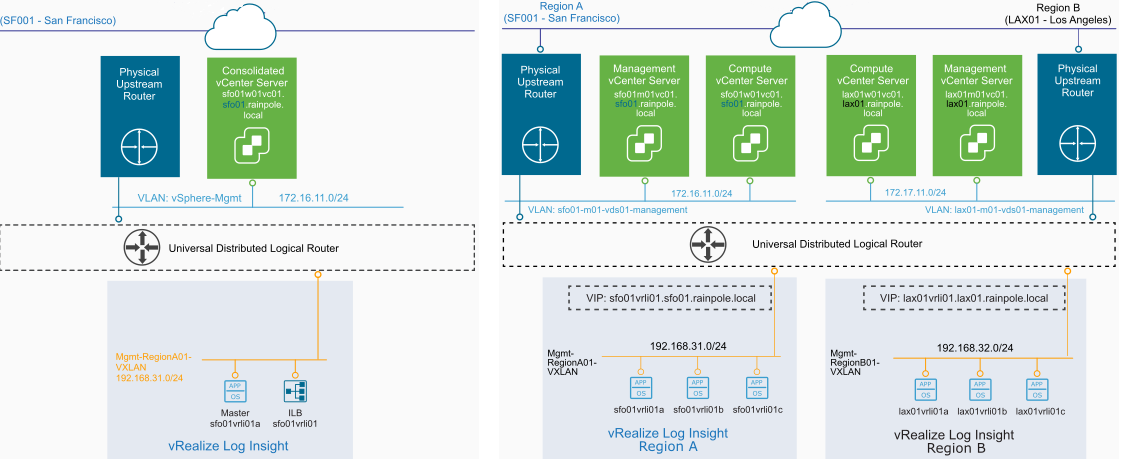
\includegraphics[width=0.7\textwidth]{imaxes/conceptosPrevios/networkLogInsight.png}
    %   \caption{Localización de vRealize Log Insight en el modelo consolidado (izquierda) y en el modelo estándar (derecha)}
    %   \label{fig:redLogIsight}
    % \end{figure}
    % \FloatBarrier
    \end{subsection}
    \end{section}
\begin{section}{Conceptos}
En este apartado se describen algunos conceptos que se deben tener claros para entender la estructura y arquitectura de los componentes de VMware Cloud Foundation.
% En este apartado se describe la arquitectura de VMware Cloud Foundation y como estructura sus componentes\footnote{Se describen solo aquellos componentes que se utilizarán en el despliegue de Cloud Foundation.} internamente.

%%%%%%%%%%%%%%%%%%%%%%%%%%%%%%
% \iffalse
% En este apartado se explican aquellos conceptos de VMware Cloud Foundation necesarios para entender su funcionamiento, configuración y requisitos de la infraestructura previos al despliegue del servicio.
% \fi
%%%%%%%%%%%%%%%%%%%%%%%%%%%%%%%%


%% Workload Ddomains %&%&%%%%
%%%%%%%%%%%%%%%%%%%%%%%%%%%%
\begin{subsection}{Workload Domain}
Un Workload Domain (WD) representa un bloque de recursos dentro del SDDC, formado por recursos físicos y virtuales, gestionados por los componentes de VCF. En cada WD se despliegan instancias de los componentes de VCF para controlar el acceso y uso de los recursos virtuales y físicos, estableciendo, además, una capa de seguridad sobre el WD. Esto permite que los recursos de cada WD se gestionen de forma separada. La función de un WD consiste en separar flujos de trabajo para determinar que recursos se dedican a la realización de determinadas tareas.
% Un \textit{workload domain} consiste en una instancia lógica de un SDDC que abarca todos o parte de los recursos de uno o más clusters, cuya función es aislar el flujo de trabajo de un usuario, aplicación o un determinado tipo de tareas. Cada \textit{workload domain} se extiende sobre varios hosts con el hipervisor ESXi, y contiene sus propias instancias de VMware vCenter Server, VMware vSAN y VMware NSX-T. Así, esta arquitectura permite establecer políticas de control específicas para un \textit{workload domain} y otras comunes para todos o varios \textit{workload domains} y específicas para cada uno de ellos a la vez que se simplifica la complejidad de la infraestructura. Existen \underline{tres tipos} de \textit{workload domains} que permiten aislar las tareas de gestión de la infraestructura del resto de flujos de trabajo. 

%% MANAGEMENT DOMAIN
\begin{subsubsection}{Management Domain}
\label{subsubsec:domainManagement}
% Este \textit{workload domain} se crea y configura automáticamente durante el proceso de despliegue de una instancia de VMware Cloud Foundation.
El Management Domain es el primer WD que se crea dentro del SDDC cuando se despliega VCF. Su finalidad es alojar todos los componentes de VCF que gestionan el propio Management Domain y al resto de WDs. Inicialmente, se despliegan las siguientes VMs de cada componente:

\begin{itemize}
  \item Una VM de SDDC Manager.
  \item Una VM de VMware vCenter Server.
  \item Tres VMs de VMware NSX-T Manager Appliance.
  \item Dos VMs de VMware NSX-T Edge.
\end{itemize}
Al contener todas las instancias de los componentes dedicados a la gestión del SDDC, todas las tareas de administración suceden dentro de este WD. De esta forma, su ejecución está centralizada, es más segura y está mejor controlada, ya que lo hacen sobre un conjunto de recursos dedicados exclusivamente a ellas.
% El administrador gestiona los recursos del Management Domain, tanto hosts como instancias de los componentes, desde VMware vSphere Client, y VMware NSX-T Manager se encarga de controlar y mantener las redes virtuales del SDDC. Con VMware SDDC Manager, el administrador gestiona de forma centralizada los aspectos que afectan al ciclo de vida de todos los componentes del SDDC.


% Incluye las siguientes instancias: SDDC Manager, vCenter Server, una instancia de NSX Manager, tres instancias de NSX Controller, dos instancias de Platform Services Controller y tres instancias de vRealize Log Insight \cite{sddcComponents} [Fig. \ref{fig:componentsMNGDomain}].\\
% Cuando se \underline{despliega \textit{management domain} se crean y configuran} de forma automatizada por SDDC Manager las siguientes máquinas virtuales (VM) de cada componente de Cloud Foundation\footnote{Las características de cada máquina virtual se refieren a los requisitos mínimos}:
% \begin{itemize}
%     \item Una VM de \textbf{SDDC Manager}: 4 vCPU, 16 GB de memoria, 800 GB de almacenamiento.
%     \item Una VM de \textbf{vCenter Server}: 4 vCPU, 16 GB de memoria, 290 GB de almacenamiento.
%     \item Dos instancias de \textbf{Platform Services Controller} (cada una): 2 vCPU, 4 GB de memoria, 60 GB de almacenamiento.
%     \item Una VM de \textbf{NSX Manager}: 4 vCPU, 16 GB de memoria, 60 GB de almacenamiento.
%     \item Tres VM de \textbf{NSX Controller} (cada una): 4 vCPU, 4 GB de memoria, 28 GB de almacenamiento.
%     \item Tres VM de \textbf{vRealize Log Insight}: 4 vCPU, 8 GB de memoria, 250 GB de almacenamiento.
% \end{itemize}

% Para desplegar el \textit{management domain} se requieren las siguientes \underline{capacidades mínimas} en la infraestructura \cite{WDminRequierements}:
% \begin{itemize}
%     \item \textbf{Hosts}: 4
%     \item \textbf{CPU} por host: Dual-socket con 8 cores por socket, en sistemas All-Flash.
%     \item \textbf{Memoria} total: 192 GB
%     \item \textbf{Almacenamiento} por host: 16 GB para el dispositivo de arranque, un NVMe o SSD para la capa de caché, dos SSD o HDD para la capa de capacidad\footnote{En total se requieren 800 GB para este \textit{workload domain}.}.
%     \item \textbf{NICs} por host: Dos NICs de al menos 10 GbE y, opcionalmente un NIC 1GbE BMC.
% \end{itemize}

% \begin{figure}[h!]
%   \centering
%   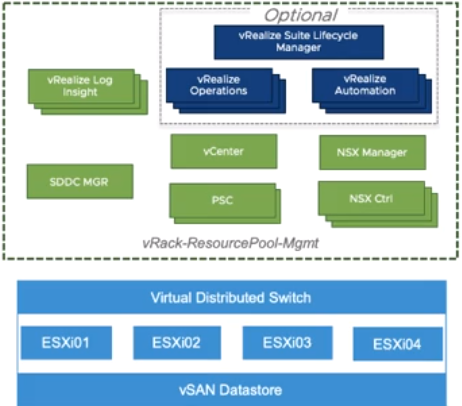
\includegraphics[width=0.5\textwidth]{imaxes/conceptosPrevios/componentsMANAGEDomain.png}
%   \caption{Componentes de \textit{management domain}}
%   \label{fig:componentsMNGDomain}
% \end{figure}
\end{subsubsection}

%% VIRTUAL INF. DOMAIN
\begin{subsubsection}{Virtual Infrastructure Domain (VI)}
\label{subsubsec:domainVI}
Este tipo de WD se crea manualmente y bajo demanda desde el Management Domain, para habilitar un entorno, cuyos recursos puedan ser usados por los usuarios mediante el despliegue de aplicaciones. Su configuración de hardware y lógica se especifican durante el proceso de creación, pudiendo establecer la cantidad de hosts, cantidad de almacenamiento, configuración de la red y políticas de rendimiento y disponibilidad, todo para satisfacer las necesidades del tipo de tareas que se van a realizar en él. Con la creación de un WD se generan las siguientes VMs:
% Con cada WD se genera un nuevo cluster de VMware vSphere que agrupa los nuevos recursos, aunque parte de sus componentes que se despliegan se controlan desde el Management Domain:
\begin{itemize}
  \item Una VM de VMware vCenter Server que se sitúa en el Management Domain.
  \item Tres VMs de VMware NSX-T Manager Appliance situadas en el Management Domain.
  \item Dos VMs de VMware NSX-T Edge.
\end{itemize}
Que ciertos componentes se sitúen en el Management Domain, permite separar las tareas de administración de un VI Domain de las aplicaciones y recursos de los usuarios, haciendo un entorno mejor organizado, más seguro y óptimo.

% El administrador gestiona los recursos del VI Domain desde VMware vSphere Client y la instancia de SDDC Manager situada en el Management Domain, y gestiona las redes virtuales del WD desde VMware NSX-T Manager situado también en el Management Domain. Los usuarios despliegan sus aplicaciones sobre los recursos de este WD, de esta forma, las tareas administrativas y las de consumo se ejecutan desde entornos separados.
% La diferencia entre un \textit{virtual infrastructure domain} y \textit{virtual desktop infrastructure domain} es que el segundo incorpora el producto VMware Horizon View que, resumiendo, permite desplegar escritorios virtuales. 
% Con cada nuevo \textit{virtual infrastructure domain} se crea un nuevo cluster vSphere en la infraestructura que agrupa todos los recursos que tiene asignados.\\
% Cuando se \underline{despliega un \textit{virtual infrastructure domain} se crean y configuran} de forma automatizada por el componente SDDC Manager las siguientes máquinas virtuales (VM) de cada componente de VMware Cloud Foundation\footnote{Las características de cada máquina virtual se refieren a los requisitos mínimos} 
%\cite{sddcComponents} [Fig. \ref{fig:compoVIdomain}]:
% \begin{itemize}
%     \item Una VM de \textbf{vCenter Server} en Management Domain: 8 vCPU, 24 GB de memoria, 500 GB de almacenamiento.
%     \item Una VM de \textbf{NSX Manager} en Management Domain: 4 vCPU, 16 GB de memoria, 60 GB de almacenamiento.
%     \item Tres VM de \textbf{NSX Controller} en el VI Domain creado (cada una):  4 vCPU, 4 GB de memoria, 28 GB de almacenamiento.
% \end{itemize}

% Por cada \textit{virtual infraestructure domain} que se despliega en la infraestructura, se requieren las siguientes capacidades mínimas\cite{WDminRequierements}:
% \begin{itemize}
%     \item \textbf{Hosts}: 3
%     \item \textbf{CPU}, \textbf{Memoria} y \textbf{Almacenamiento}: depende de los requisitos de las tareas que se vayan a desarrollar en este \textit{workload domain}.
%     \item \textbf{NICs} por servidor: Dos NICs de al menos 10 GbE y, opcionalmente un NIC 1 GbE BMC.
% \end{itemize}


 \end{subsubsection}

\end{subsection}
% \begin{figure}[h!]
%   \centering
%   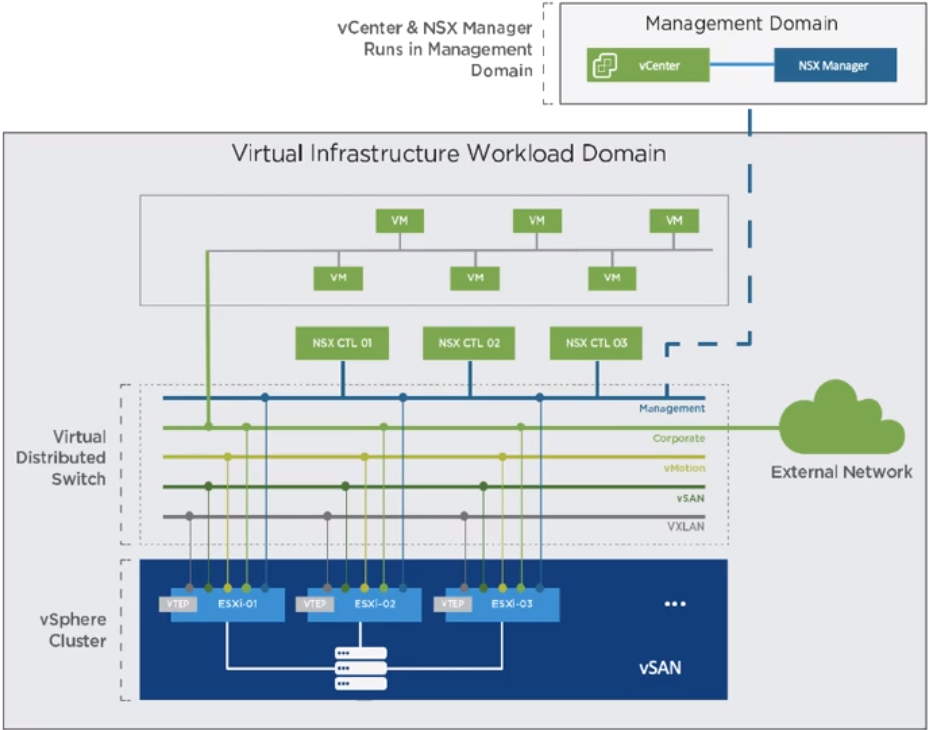
\includegraphics[width=0.5\textwidth]{imaxes/conceptosPrevios/networkArcVIDomain.png}
%   \caption{Componentes de \textit{virtual infrastructure domain}.}
%   \label{fig:compoVIdomain}
% \end{figure}
%\FloatBarrier

%&%%%%%%%%%%%%%%%%%%%%%%%%%%%%%%%%%%%%%%%%%%%%%%%%%%%%%%%%
%% ARQUITECTURA



\begin{subsection}{Arquitectura}
VMware proporciona dos posibles modelos de arquitectura diferentes. Se utiliza uno u otro dependiendo del tamaño de la infraestructura sobre la que se va a desplegar VCF, y con cada modelo, se determina la forma en la que se agruparán y administrarán los recursos del SDDC.

%%%%%%%%%%%%%%%%%%%%%
%%%%%%%%%%%%%%%%%%%%%%%%
%% ESTANDAR
\begin{subsubsection}{Modelo estándar}

Este modelo está pensado para entornos de tamaño medio/grande, con un mínimo de siete hosts. Está formado por un Management Domain y al menos un VI Domain. Esto implica que la ejecución de tareas dentro de un WD está limitada por los recursos que lo forman. Esto permite asignar roles a los recursos según las operaciones que se van a ejecutar sobre ellos, establecer un nivel de seguridad en cada WD y dedicar un conjunto de recursos a la ejecución de cierto tipo de operaciones. Así, el entorno es más eficiente, ya que se proporciona una forma de adecuar la configuración de los recursos de acuerdo con el uso que se va a hacer del servicio o servicios desplegados, minimizando además los cambios sobre la infraestructura física.
% esde el Management Domain se administra toda la infraestructura del SDDC y cada VI Domain existente, los cuales son creados bajo demanda desde el Management Domain y sus recursos se establecen según su finalidad. Un Management Domain puede gestionar hasta un máximo de de catorce VI Domain. 
%Cada \textit{virtual infrastructure domain} requiere tres hosts adicionales, es decir, un host solo puede pertenecer a un único \textit{workload domain}. 

\begin{figure}[h!]
  \centering
  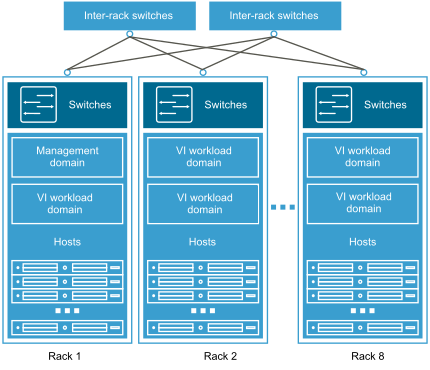
\includegraphics[width=0.6\textwidth]{imaxes/conceptosPrevios/arquitect_standarCF.png}
  \caption{Esquema del modelo de arquitectura estándar.}
  \label{fig:modelostandard}
\end{figure}

% \begin{figure}[h!]
%   \centering
%   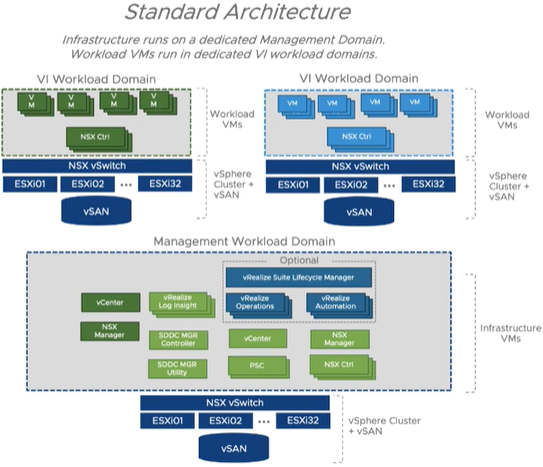
\includegraphics[width=0.6\textwidth]{imaxes/conceptosPrevios/standardArch.png}
%   \caption{Estructura de los componentes en una arquitectura estándar.}
%   \label{fig:standardarch}
% \end{figure}
\FloatBarrier
%%%%%%%%%%%%%%%%%%%%%
%%  CONSOLIDADO
\end{subsubsection}
\begin{subsubsection}{Modelo consolidado}
Este modelo está orientado a entornos de tamaño pequeño, con menos de siete hosts. Está formado por un único WD que cumple las funciones de un Management Domain y de un VI Domain, es decir, en él se colocan las instancias de los componentes dedicados a la gestión del SDDC\footnote{Se despliega la misma cantidad de instancias que en el Management Domain.} junto con las aplicaciones desplegadas para la realización de otro tipo de tareas. Así, a diferencia del modelo estándar, todas las operaciones se ejecutan dentro de un mismo entorno y sobre los mismos recursos. Internamente, las VMs se pueden colocar dentro de un grupo, llamado \textit{resource pools}, en el que se puede establecer un límite de uso de recursos.
Este modelo no aporta tantos beneficios como el modelo estándar, ya que todas las operaciones se realizan sobre los mismos recursos, y los niveles de control y seguridad son menores, por lo tanto su uso solo está recomendado para entornos de tamaño reducido.
% Dentro del cluster de VMware vSphere que se crea, las instancias pertenecientes a los componentes de administración del SDDC y las pertenecientes al trabajo de los usuarios, se colocan en \textit{resource pools} separados. Un \textit{resource pool} es un elemento de VMware vSphere que permite establecer unos límites de consumo de recursos sobre las instancias que se sitúan en su interior\cite{resourcePool}.

% Este modelo está pensado para desplegar VMware Cloud Foundation en entornos de tamaño pequeño, normalmente cuando hay menos de siete hosts, aunque también se puede utilizar en entornos más grandes con hasta 64 hosts. En este modelo los flujos de trabajo que corresponden al \textit{virtual infrastructure domain} y al \textit{management domain} en el despliegue estándar, están colocados dentro de un mismo \textit{workload domain} en un único cluster pero aislados gracias a que cada uno se coloca dentro de un \textit{resource pool} diferente, es decir, existe un cluster con varios \textit{resource pool}. El modelo consolidado se convierte en un modelo estándar cuando se añade un \textit{workload domain} al SDDC.[Fig. \ref{fig:modeloconsolidated}].

\begin{figure}[h!]
  \centering
  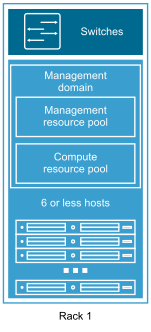
\includegraphics[width=0.25\textwidth]{imaxes/conceptosPrevios/modelConsolidated.png}
  \caption{Esquema del modelo de arquitectura consolidado.}
  \label{fig:modeloconsolidated}
\end{figure}

% \begin{figure}[h!]
%   \centering
%   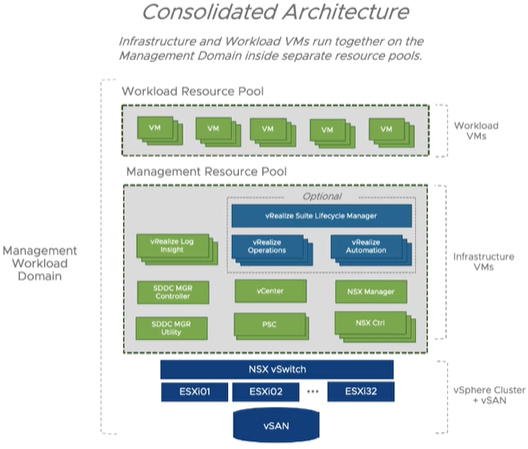
\includegraphics[width=0.6\textwidth]{imaxes/conceptosPrevios/consolidatedArch.png}
%   \caption{Estructura de los componentes de una arquitectura consolidado.}
%   \label{fig:consolidatedArch}
% \end{figure}
\FloatBarrier

\end{subsubsection}
\end{subsection}

\begin{subsection}{Clusters, zonas y distribución de un SDDC}

  Los recursos de un SDDC pueden estar distribuidos en diferentes localizaciones para proporcionar mayor disponibilidad y recuperación ante fallos. Estos recursos, se agrupan para formar una estructura que permite usar y gestionar los recursos disponibles de forma conjunta y dinámica.

\begin{subsubsection}{Availability Zone, Region y Cluster}
\begin{itemize}
  \item Availability Zone (AZ): se llama AZ a un conjunto de recursos físicos que forman una infraestructura independiente, es decir, cada una tiene su propia fuente de energía, su sistema de refrigeración, su sistema de seguridad y su red, no compartidos con otra AZ, para evitar la propagación de fallos hacia otras AZs. Cuando existen varias AZs, se pueden usar de forma que cuando ocurre un fallo en una de ellas la carga de trabajo se distribuye a una segunda AZ y, así, minimizar el tiempo de caída del servicio. Dentro de una AZ se alojan uno o más WDs.
  
  \item Region: se llama Region a un conjunto de AZs situadas en una misma ubicación, es decir, las AZs de una Region están situadas próximas entre sí. Estas AZs deben tener al menos una latencia de 5 ms entre ellas. Dentro de un SDDC pueden existir varias Regions pero estas se sitúan en ubicaciones más distantes, la latencia debe ser de al menos 150 ms. Esta estructura permite ofrecer los servicios de un SDDC en diferentes ubicaciones, a la vez que se aumenta su disponibilidad y recuperación ante fallos.
  
  \item Cluster: un cluster de VMware vSphere es una agrupación de hosts. A las instancias desplegadas sobre ellos, se les aplica una configuración de disponibilidad con el componente VMware vSphere, permitiendo determinar como se restablecen las instancias cuando ocurre un fallo dentro del cluster. Un cluster se sitúa dentro de un WD, por lo tanto, sus recursos estarán limitados por el alcance del WD. 
  %  Esta estructura permite acercar el servicio a ubicaciones separadas por grandes distancias. La arquitectura del modelo consolidado solo soporta una Region con una AZ, mientras que el modelo estándar permite desplegar múltiples Regions con múltiples AZs.
\end{itemize} 

\begin{figure}[h!]
  \centering
  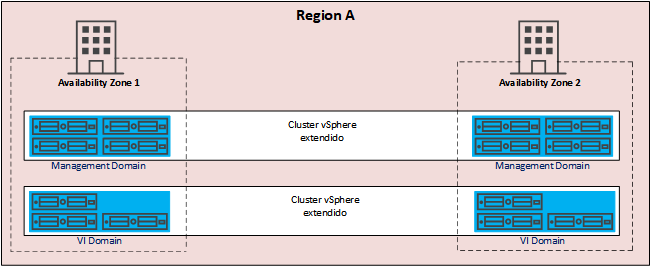
\includegraphics[width=0.8\textwidth]{imaxes/conceptosPrevios/AZRegionCluster.png}
  \caption{Ejemplo de un SDDC con dos Regions y una AZ en cada uno.}
  \label{fig:az-region-cluster}
\end{figure}
En la figura anterior se describe el esquema de un SDDC compuesto de una Region. Dentro de esta, existen dos AZ, AZ1 y AZ2. Cada una de las AZs contiene dos WD, un Management Domain desde donde se administra el SDDC, y un VI Domain donde se realizan las operaciones del SDDC. Como se mencionaba anteriormente, las instancias situadas en una AZ pueden migrar de una ubicación a otra en caso de fallo de los recursos físicos. Para ello, el WD donde se encuentran esas instancias debe estar extendido en las dos AZs. En la imagen, el Management Domain está formado por ocho hosts, repartidos en las AZs, los cuales están agrupados dentro del mismo cluster de VMware vSphere, por lo tanto, los componentes cuyas instancias estén situadas en este cluster se podrán migrar entre los 8 hosts. Estas migraciones se realizan en función de la configuración de disponibilidad establecida en los componentes VMware vSphere y VMware vSAN. Así, cuando los hosts de AZ1 sufren una caída, la AZ2 seguiría activa y las instancias situadas en AZ1 migrarían a AZ2 para continuar la disponibilidad del servicio, todo esto de forma automatizada, dinámica y transparente para el usuario. Lo mismo sucedería con el VI Domain\footnote{Se puede encontrar una descripción más detallada de esta estructura en el siguiente enlace \url{https://docs.vmware.com/en/VMware-Validated-Design/6.0/introducing-vmware-validated-design/GUID-661B1CE3-1F74-4E00-80F3-0F5EA39528CD.html}}.


\end{subsubsection}
% \begin{subsubsection}{Cluster y Resource Pool}
% Dentro de un \textit{workload domain} pueden existir varios clusters. Un cluster es una agrupación de hosts a cuyos recursos se les puede aplicar una una configuración de disponibilidad determinada con los componentes VMware vSphere High Availability y VMware vSphere Distributed Resource Scheduler para establecer como se restablece el servicio en caso de fallos en alguno de los hosts. Un cluster puede estar extendido en más de una AZ para que si una de las AZs falla, las aplicaciones que corrían en ella pueden ser migradas a otra AZ mejorando la disponibilidad del servicio. En un WD se despliegan dos clusters:
% \begin{itemize}
%   \item Management cluster: es el cluster que se crea al desplegar VMware Cloud Foundation. Contiene los componentes para administrar los recursos del WD.
%   \item Shared Edge and Workload Cluster: después del management cluster, este es el primero que se crea. Su finalidad es alojar las aplicaciones y cargas de trabajo de los usuarios dentro de un WD. Además contiene instancias de Vmware NSX-T para proporcionar sevicios de red.
% \end{itemize}

% Dentro de un cluster se pueden crear resource pools. Un \textit{resource pool} es una característica de VMware vSphere que permite abstraer un conjunto de recursos de un cluster estableciendo unos límites de capacidad que puede usar \cite{resourcePool}. Usar resource pools permite agrupar las VMs con una finalidad similar y controlar la cantidad de recursos del WD que esas VMs pueden consumir.

% Un SDDC puede estar distribuído en una o más \textit{Availability Zone} (AZ). Estas son zonas aisladas con infraestructuras independientes que evitan la propagación de fallos de hosts individuales a través de toda la infraestructura, cuantas más \textit{AZ} existan mayor disponibilidad tendrá el servicio. La latencia entre dos \textit{AZ} debe ser de 5 ms como máximo y la conexión de al menos 10 Gbit. Una \textit{Region} agrupa una o más \textit{AZ}s, con esto se da solución a la recuperación del servicio ante desastres. La latencia entre dos \textit{Region}s debe ser de 100 ms como máximo. El \underline{modelo consolidado} solo da soporte a una \textit{Region} con una \textit{AZ}, mientras que el \underline{modelo estándar} puede soportar múltiples \textit{Region} con múltiples \textit{AZ}.
% \end{subsubsection}
\end{subsection}

\end{section}

% \subsubsection{Clusters, zonas de disponibilidad y regiones}
% Un SDDC puede estar formado por uno o más clusters de distintos tipos. En el  \underline{modelo consolidado} la infraestructura está formada por un único cluster que incluye los servicios de gestión de VMware Cloud Foundation VMware vCenter Server, vSphere Update Manager, VMware NSX Manager, VMware NSX Controller y VMware vRealize Log Insight, los servicios de red necesarios para establecer conectividad en el entorno y las máquinas virtuales que los usuarios crean cuando aprovisionan sus recursos. Se aplican las mismas políticas de alta disponibilidad y gestión del ciclo de vida al flujo de trabajo de gestión del SDDC y al flujo de trabajo del usuario. En el \underline{modelo estándar} los distintos \textit{workload domain} se dividen en clusters que pueden ser de tres tipos:
%     \begin{itemize}
%         \item \textbf{Management Cluster}: se crea durante el despliegue de VMware Cloud Foundation y contiene el \textit{management domain}, desde aquí se gestiona el SDDC. Contiene los servicios de gestión mecionados anteriormente.
%         \item \textbf{Shared Edge and Compute Cluster}: es el primer cluster que se crea dentro de un \textit{virtual infrastructure domain} ya que puede haber más de un cluster. Este cluster contiene los servicios de red NSX del \textit{workload domain} y también puede contener el flujo de trabajo de los usuarios.
%         \item \textbf{Compute Cluster}: cluster adicional que se crea dentro de un \textit{virtual infraestructure domain}. Contiene el flujo de trabajo de los usuarios.
%     \end{itemize}
% Un SDDC puede estar distribuído en una o más \textit{Availability Zone} (AZ). Estas son zonas aisladas con infraestructuras independientes que evitan la propagación de fallos de hosts individuales a través de toda la infraestructura, cuantas más \textit{AZ} existan mayor disponibilidad tendrá el servicio. La latencia entre dos \textit{AZ} debe ser de 5 ms como máximo y la conexión de al menos 10 Gbit. Una \textit{Region} agrupa una o más \textit{AZ}s, con esto se da solución a la recuperación del servicio ante desastres. La latencia entre dos \textit{Region}s debe ser de 100 ms como máximo. El \underline{modelo consolidado} solo da soporte a una \textit{Region} con una \textit{AZ}, mientras que el \underline{modelo estándar} puede soportar múltiples \textit{Region}s con múltiples \textit{AZ}s.

%%%%%%%%%%%%%%%%%%%%%%%%%%%%%%%%%%%%%%%%%%%%
%%%%%%%%%%%%%%%%%%%%%%%%%%%%%%%%%%%%%%%%%%%%
%%%%%%%%%%%%%%%%%%%%%%%%%%%%%%%%%%%%%%%%%%%%
% \iffalse
% Un SDDC puede estar \underline{formado por múltiples clusters} que pueden ser de diferentes tipos con diferentes propósitos. Un cluster puede ocupar uno o más \textit{racks} dependiendo del nivel de escalabilidad que se requiera. Según su función, cada \textit{workload domain} se puede colocar en un cluster diferente para gestionar la alta disponibilidad y el ciclo de vida según sus necesidades. Un \underline{cluster puede ser de varios tipos}:
% \begin{itemize}
%     \item \textbf{Management Cluster}: Es aquel que contiene el \textit{management domain}, por lo tanto contiene las máquinas virtuales de los componentes que gestionan el SDDC. A este cluster solo deben acceder los administradores de la infraestructura.
%     \item \textbf{Shared Edge y Compute Cluster}: contiene el \textit{virtual infrastructure domain} con las máquinas virtuales de los usuarios y, además, incorpora servicios de NSX necesarios para comunicarse con redes externas y con otros \textit{workload domains}.
%     \item \textbf{Compute Cluster}: solo contiene el \textit{virtual infrastructure domain} con las máquinas virtuales de los usuarios.
%     \item \textbf{External Storage}: se centra en proveer almacenamiento de tipo NFS, iSCSI o Fiber Channel.
% \end{itemize}

% Un SDDC puede estar distribuído en una o más \underline{zonas de disponibilidad}. Estas son zonas aisladas que evitan la propagación de fallos de hosts individuales a través de toda la infraestructura, así, se puede entregar mayor disponibilidad de los recursos y servicios. A su vez, varias \underline{zonas de disponibilidad} se pueden agrupar en una \underline{región}, estos entornos separados por grandes distancias que permiten tener recuperación ante desastres [Fig. \ref{fig:AVRegiones}].\\

% \begin{figure}[h!]
%   \centering
%   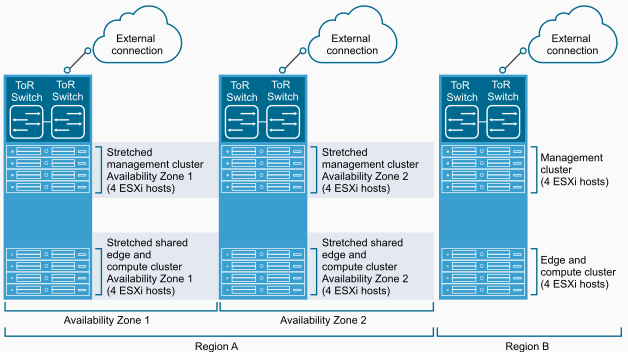
\includegraphics[width=0.95\textwidth]{imaxes/conceptosPrevios/zonasDispRegiones.png}
%   \caption{Una región contiene al menos una zona de disponibilidad.}
%   \label{fig:AVRegiones}
% \end{figure}
% \fi
%%%%%%%%%%%%%%%%%%%%%%%%%%%%%%%%%%%%%%%%%%%%%
%%%%%%%%%%%%%%%%%%%%%%%%%%%%%%%%%%%%%%%%%%%%%
%%%%%%%%%%%%%%%%%%%%%%%%%%%%%%%%%%%%%%%%%%%%%



\begin{section}{Requisitos}
En este apartado se describe aquello que debe cumplir la infraestructura física para que los componentes de VMware Cloud Foundation funcionen de forma adecuada y que la configuración y mantenimiento de los componentes físicos sea sencilla a la hora de expandir el entorno.

% Teniendo en cuenta las capacidades físicas de la infraestructura, se ha elegido el modelo consolidado para el despliegue de VMware Cloud Foundation sobre la infraestructura.     La principal razón por las que se escoge este modelo es por el número de hosts ESXi.
% En los siguientes apartados se describen la arquitectura que se genera y la infraestructura requerida en cada capa.
%%%%%%%%%%%%%%%%%%%%%%%%%%%%%%%%%%%%%%
\begin{subsection}{Cómputo}
\begin{subsubsection}{Hosts ESXi}
    Para realizar el despliegue del primer WD (el Management Domain) se requieren al menos cuatro hosts ESXi con al menos 128 GB de memoria RAM y un disco de arranque de 32 GB cada uno\footnote{Según la configuración establecida para el producto vSAN ReadyNode \cite{host-requirements}}. Para cada WD adicional solo se requiere un mínimo de tres hosts cuya cantidad de memoria RAM depende de la finalidad del WD. Cada uno de los hosts debe tener al menos dos interfaces de red físicas (NIC) que soporten al menos 10 Gbit/seg de velocidad.
    
\end{subsubsection}
\end{subsection}
%%%%%%%%%%%%%%%%%%%%%%%%%%%%%%%%%%%%%%%
\begin{subsection}{Almacenamiento}
    En el Management Domain es obligatorio el uso de un \textit{datastore} de VMware vSAN, este necesita al menos tres hosts con recursos de almacenamiento para funcionar\footnote{VMware vSAN requiere un mínimo de tres hosts mientras que el Management Domain requiere un mínimo de cuatro hosts.}. Se debe aplicar la configuración All-Flash con discos SSD. Basándose en los perfiles que VMware establece para su producto vSAN Ready Node\cite{host-requirements}, cada host debe tener al menos un grupo de dos discos donde la cantidad de almacenamiento para la capa de capacidad debe ser de 4 TB y para la capa de caché de 200 GB. VMware vSAN soporta discos con adaptadores SAS, SATA o SCSI y estos pueden estar configurados en modo \textit{pass-through} o RAID 0. En cuanto a esto, es preferible que los discos se configuren en modo \textit{pass-through} ya que permite que estos se puedan gestionar de forma independiente, sin tener que apagar los hosts cuando sea necesario retirar o añadir discos.
    Para WDs adicionales se puede utilizar almacenamiento NFS en lugar de un datastore de VMware vSAN, aunque la solución de VMware aporta mayor rendimiento y simplifica la administración de esta parte de la infraestructura física.
    % los discos de caché debe ser al menos un 10\% del tamaño total de los discos de capacidad,  y  \footnote{La capacidad de los discos descrita es la necesaria para desplegar el \textit{management domain} y un \textit{workload domain} adicional.}
\end{subsection}
%%%%%%%%%%%%%%%%%%%%%%%%%%%%%%%%%%%%%%%
\begin{subsection}{Red}
 \begin{subsubsection}{Switch Top Of Rack}
     Los hosts están colocados en racks, en un rack puede haber hosts pertenecientes a distintos WD. Para favorecer la alta disponibilidad y tolerancia a fallos de la infraestructura física, un rack debe tener dos switches Top Of Rack (TOR) y cada host debe tener una interfaz conectada a cada uno de ellos, una capa superior de switches conecta los switches TOR entre sí. Todas las conexiones de la red física deben soportar \textit{Jumbo frames} (MTU hasta 9000 Bytes), etiquetado \textit{Quality of Service} (QoS) de tráfico y el etiquetado VLAN, todo para dar soporte a las subredes del SDDC. Todas las conexiones físicas deben tener, al menos, 10 Gbit/seg de velocidad.
    % Todos los switches TOR deben tener al menos dos interfaces 10 Gbit Ethernet como mínimo. 
    % \footnote{Para el Management Domain, las subredes cuya VLAN debe ser configurada en la red física son la subred Management para tareas de administración, la subred dedicada a VMware vSAN, la subred dedicada a overlay y la subred dedicada a VMware vSphere vMotion.}
 \end{subsubsection}
 \begin{subsubsection}{Servicios}
     En el SDDC se deben habilitar varios servicios requeridos por los componentes de VMware Cloud Foundation para su correcto funcionamiento.
     \begin{itemize}
         \item DNS: servidor de nombres para resolver todas las direcciones IP y \textit{hostnames} de los componentes del SDDC.
         \item DHCP: servidor para asignar de forma automática una dirección IP a los hosts que forman el SDDC.
         \item NTP: servidor de tiempo para sincronizar la hora de todos los componentes del SDDC.
         \item Router: se requiere para enrutar el tráfico que emiten todas las instancias del SDDC y para dar acceso a redes externas. Debe soportar enrutamiento dinámico BGP y debe tener configuradas las subredes y VLANS que se vayan a utilizar en la infraestructura.
         \item SMTP: servidor de correo utilizado para el envío de alertas y comunicación de los usuarios con el administrador del SDDC.
         \item Active Directory: servidor de usuarios y grupos de usuarios que el SDDC utiliza como fuente para configurar el acceso a cada parte de la infraestructura virtual.
         \item Certificate Authority: se debe configurar una autoridad certificadora que genere certificados firmados para cada uno de los componentes de VMware Cloud Foundation. Permite establecer conexiones seguras cuando se accede a los componentes.
     \end{itemize}
 \end{subsubsection}
\end{subsection}


\end{section}
%%%%%%%%%%%%%%%%%%%%%%%%%%%%%%%%%%%%%%%
    %%%% DISEÑO ARQUI. FÍSICA %%%%%
% \begin{subsection}{Arquitectura e Infraestructura Físicas \cite{CFfisInfraestuctura}}
%     En este apartado se describen las principales características que tiene el entorno físico de un SDDC construído con VMware Cloud Foundation.


% \begin{subsubsection}{Red física}
% La topología de red en la capa física del SDDC de VMware Cloud Foundation se puede implementar mediante servicios de \underline{transporte} en la capa 2 o en la capa 3. El \underline{diseño en la capa 2} implica que la topología de la red incluya los dispositivos de capa 2 (\textit{Top of Rack Switches}) y los dispositivos de la capa 3 (routers, switches) [Fig. \ref{fig:transportlayer2}], por lo tanto las VLANs que se definan se deben implementar en la capa 2 y en la capa 3. Esto puede provocar problemas al aumentar el tamaño de la red ya que el número de VLANs disponible es más limitado, y problemas de compatibilidad ya que es posible que los dispositivos físicos tengan que ser del mismo proveedor. El \underline{diseño en la capa 3} implica que la topología de la red solo incluye a los dispositivos de capa 3 [Fig. \ref{fig:transportlayer3}]. Esto permite limitar la definición de VLANs a esa capa y el uso de enrutamiento dinámico con protocolos OSPF o BGP entre la capa 2 y 3. Así se consigue una mayor libertad a la hora de seleccionar los dispositivos físicos de red y que su configuración es más sencilla.
% \begin{figure}[h!]
%   \centering
%   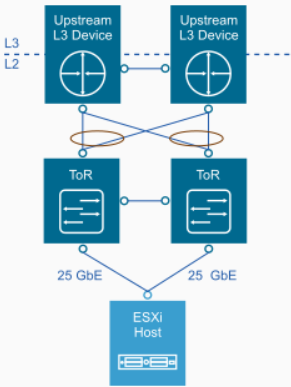
\includegraphics[width=0.3\textwidth]{imaxes/conceptosPrevios/transportlayer2.png}
%   \caption{Límite de las capas 2 y 3 cuando la topología se implementa con dispositivos de capa 2.}
%   \label{fig:transportlayer2}
% \end{figure}
% \FloatBarrier
% \begin{figure}[h!]
%   \centering
%   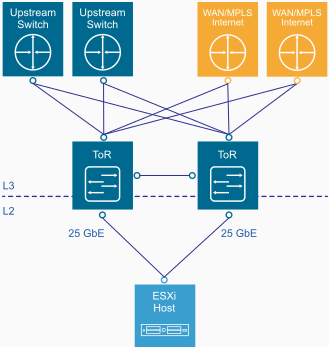
\includegraphics[width=0.3\textwidth]{imaxes/conceptosPrevios/transportNetLayer3.png}
%   \caption{Límite de las capas 2 y 3 cuando la topología se implementa con dispositivos de capa 3.}
%   \label{fig:transportlayer3}
% \end{figure}
% \FloatBarrier



% Como VMware Cloud Foundation abstrae la red física en una red virtual, la red física debe cumplir ciertos requisitos para que la red virtualizada sea robusta. Esta se debe mantener simple con configuraciones comunes en todos los switches, uso de VLANs y uso de enrutamiento dinámico, también debe ser escalable en cuanto a cantidad de hosts, ancho de banda y cantidad de rutas redundantes. Además, se debe tener en cuenta que cada tipo de tráfico tiene características diferentes, como por ejemplo el tráfico dedicado al almacenamiento a través de IP que suele usar mayor ancho de banda, por ello es necesario distinguir cada tipo de tráfico con protocolos \textit{Quality of Service} (QoS). El marcado de cada tipo de tráfico se realiza en el hipervisor ESXi a través de un vSphere Distributed Switch que soporta QoS tanto en la capa 2 como en la capa 3. En la capa 2 se utiliza  un campo de tres bits llamado \textit{Class of Service} que representa la prioridad del \textit{frame} con un valor de cero a siete, presente en la cabecera Ethernet cuando se utiliza etiquetado VLAN, mientras que en la capa 3 se utiliza un campo de 6 bits en la cabecera IP llamado \textit{Differentiated Services Code Point}, perteneciente al protocolo \textit{DiffServ}, para clasificar cada paquete. Los \underline{principales componentes que se deben configurar} para dar conectividad entre los servidores son los siguientes:
% \begin{itemize}
%     \item \textbf{Top of Rack Physical Switches} (TOR): es un switch al que se conectan los hosts de un rack para tener conectividad con el resto de la infraestructura. Se recomienda que un host esté conectado a dos switches TOR y que estos se configuren de forma redundante para proveer alta disponibilidad y tolerancia a fallos de alguna de las conexiones. Cada switch TOR se conecta a otro par de switches que establece conexión entre todos los racks.
    
%     Los puertos del switch TOR que se conectan a los hosts deben estar configurados como puertos troncales de VLAN para que acepte todas las VLANs usadas por el host, se debe proveer servicio DHCP a cada VLAN usada y configurar los puertos para que acepten \textit{jumbo frames}. El marcado QoS del tráfico que realiza cada host ESXi debe ser aceptado y no puede ser modificado una vez abandona el host. 
%     % \iffalse Además, se deben configurar todas las VLANs y subredes que se utilizarán en la infraestructura de VMware Cloud Foundation.\fi  
    
%     \underline{Otros protocolos que se deben configurar} en los puertos que se conectan con los hosts son:
%     \begin{itemize}
%         \item \emph{Spanning Tree Protocol} (STP): protocolo que se encarga de gestionar las rutas de la red que son redundantes.
%         \item \emph{Trunking}: configurar cada enlace troncal con las VLANs que van a transmitir tráfico a través de él. Se debe establecer como VLAN nativa, aquella utilizada para transmitir el tráfico que no tiene etiqueta, VLAN de la red \textit{management}.
%         \item \emph{MTU}: configurar el MTU de cada VLAN para el transporte de paquetes \textit{jumbo frames}. Este valor será el que se use para configurar los hosts ESXi. Se recomienda establecerlo en 9000 bytes.
%         \item \emph{Multicast}: configurar el protocolo IGMP en cada switch TOR como enrutador (busca activamente que VLANs pertenecen a un grupo Multicast) y cada VLAN como miembros de IGMP (los hosts que forman parte del grupo indican su pertenencia a un grupo multicast de forma activa).
%     \end{itemize}
    

    
%     % \iffalse
%     % \item \textbf{Conectividad entre Regiones}: 
%     % \item \textbf{Conectividad entre Zonas de dispobilidad}:
%     % \fi
% \end{itemize}

% Los siguientes servicios usados por los componentes de VMware Cloud Foundation se deben configurar sobre la red física de la infraestructura para el correcto funcionamiento del SDDC\cite{CFexternalServices}:
% \begin{itemize}
%     \item \textbf{Servidor DNS}: se utiliza para obtener los nombres y direcciones de todas las máquinas virtuales que se creen, tanto en sentido \textit{fordward} (obtener una dirección IP a partir de un nombre) como en sentido \textit{reverse} (obtener un nombre a partir de una dirección IP). Además, este servicio debe ser configurado antes de realizar el despliegue de VMware Cloud Foundation. Este servicio es utilizado por el componente Platform Services Controller, vCenter Server, NSX Manager y vRealize Log Insight.
    
%     \item \textbf{Servidor DHCP}: permite asignar direcciones IP de forma dinámica a los puertos \textit{vmkernel} de cada host ESXi. Este debe ser accesible desde cada VXLAN de VMware NSX y es necesario establecer previamente las redes que se van a usar en VMware Cloud Foundation. Este servicio debe estar disponible antes de comenzar el despliegue del SDDC ya que es necesaria la asignación dinámica de IPs.
    
%     \item \textbf{Servidor NTP}: requerido por todos los componentes de VMware Cloud Foundation para mantener sus horas sincronizadas. Este servicio debe estar disponible en la infraestructura y configurado en cada host ESXi antes del despliegue de VMware Cloud Foundation, y debe ser alcanzable desde la red de \textit{management} y de vRealize. La derencia de tiempo entre los componentes de la infraestructura no debe ser mayor de cinco minutos.
    
%     \item \textbf{Router}: debe existir enrutamiento dinámico en la red desde la capa 3. Es requerido por NSX para establecer comunicación con los ESG. Este servicio debe estar configurado antes del comenzar enl despliegue de VMware Cloud Foundation. 
% \end{itemize}

% \end{subsubsection}


% \begin{subsubsection}{Host ESXi\cite{WDminRequierements}}
% Los hosts ESXi que se desplieguen en un cluster deben tener características físicas idénticas para hacer la infraestructura más manejable,  incluyendo la configuración de almacenamiento y red. Para desplegar VMware Cloud Foundation se requiere:
% \begin{itemize}
%     \item  Dos interfaces de red (NIC) de la misma velocidad que deben estar conectadas a la VLAN troncal de dos switches TOR. Configurando \textit{NIC teaming} en VMware Sphere Distributed Switch se consigue que el tráfico se distribuya por las interfaces de red disponibles de forma óptima y que exista tolerancia a fallos.
%     \item Todas las conexiones físicas del host deben tener al menos una velocidad igual a 10 Gbit.
%     \item Cada host debe tener al menos 192 GB de memoria RAM, de esa cantidad, 176 GB de memoria RAM son requeridos por las máquinas virtuales que gestionan el SDDC.
%     \item Un disco de arranque con un tamaño mínimo de 16 GB.
% \end{itemize}

% \end{subsubsection}


% \begin{subsubsection}{Almacenamiento físico}
% VMware Cloud Foundation utiliza VMware vSAN para proveer el almacenamiento de un SDDC. Para desplegar VMware Cloud Foundation, VMware vSAN requiere las siguientes características:
% \begin{itemize}
%     \item Mínimo de tres hosts con recursos de almacenamiento.
%     \item Determinar qué configuración de vSAN se va a utilizar, \textit{All-Flash} o \textit{Hybrid}. Se recomienda la solución \textit{All-Flash} ya que ofrece mayor rendimiento.
%     \item Para cada host con recursos de almacenamiento se debe cumplir que el disco de caché tenga un 10\% de la capacidad del almacenamiento persistente del grupo de discos, tener un mínimo de dos discos en la capa de capacidad, un controlador RAID y configurar habilitar vSphere High Availability  para apagar las máquinas virtuales de un host cuando este se encuentre aislado. El controlador RAID debe tener la característica \textit{pass-through} la cual permite que VMware vSAN muestre como discos individuales cada disco duro de un grupo de discos, esto facilita la gestión de cada disco y que se puedan realizar sustituciones sin detener el servicio.
%     \item La capacidad mínima de almacenamiento disponible para el modelo consolidado es de 800 GB. 
% \end{itemize}

% \end{subsubsection}

% \end{subsection}

\begin{section}{Prueba de concepto}
Para no afectar al funcionamiento del servicio proporcionado por el CITIC y para mostrar y probar las capacidades de VMware Cloud Foundation, en lugar de utilizar un entorno real el proyecto se lleva a cabo en un entorno aislado de prestaciones reducidas. Siguiendo la metodología Scrum, primero se deplegará VMware Cloud Foundation con la herramienta VMware Lab Constructor (VLC)\footnote{Se utiliza la versión 4.0.1 del instalador.}, que genera de forma automatizada una infraestructura física embebida basada en el diseño propuesto por VMware y sobre la cual posteriormente despliega los componentes base de VCF. Después se añadirá el componente que permite la gestión de usuarios y finalmente el servicio de aprovisionamiento. Una vez desplegados todos los elementos se realizará una demostración del servicio.
% Una vez generado se instalarán las aplicaciones necesarias para gestionar los usuarios del sistema y el servicio de aprovisionamiento.

\begin{subsection}{Preparación}
  \begin{subsubsection}{Host ESXi}  
  
  Como base para la instalación se utiliza un servidor físico con el hipervisor ESXi instalado que aunque no cumpla con alguno de requisitos mínimos de VMware Cloud Foundation, no aporta gran rendimiento pero si permite crear un entorno funcional a modo de prueba. Este host cuenta con una memoria RAM de 128 GB, una CPU de 28,8 GHz y un \textit{datastore} con discos SSD con 2 TB de capacidad. Cuenta con dos interfaces físicas, una que conecta al host con el \textit{datastore} y otra a la que se conectan dos redes, una llamada \textit{Management Network} que permite acceder al host desde una VM para gestionarlo, y otra llamada \textit{VM Network} donde se conectan todas las VMs generadas por VLC y de los servicios que dan soporte a los componentes de VMware Cloud Foundation.
  \end{subsubsection}
  \begin{subsubsection}{Servicios}
    Todos los servicios requeridos por VMware Cloud Foundation se despliegan sobre el mismo servidor en forma de VMs. Una de las VMs es Windows Server 2016 que contiene un servidor DNS, un servidor NTP, un servidor Active Directory, un servidor SMTP y ejerce también como Certificate Authority. Otra VM contiene el sistema operativo VyOS que funciona como un router virtual y como servidor DHCP. Una última VM con Windows 10\footnote{Se refiere a ella como \textit{Jump Host}.} se requiere para ejecutar VLC y acceder al entorno embebido generado por VLC.
    El servidor DNS contiene los \textit{hostnames} y sus respectivas direcciones IP de todas las VMs, tanto las que residen dentro del host físico como las que se alojan dentro del entorno embebido generado por la herramienta VLC. Este servidor DNS implementa un único dominio que se denomina \textit{pesci.domain}. El servidor Active Directory proporciona almacena usuarios y grupos de usuarios requeridos para establecer roles y proporcionar acceso a los componentes y servicios de VMware Cloud Foundation. Se utiliza este servidor de usuarios en lugar del directorio real de la UDC para evitar posibles problemas del servicio. El router VyOS tiene configuradas todas las subredes y VLANs que VMware Cloud Foundation utiliza en la capa L3 de la infraestructura física y proporciona acceso a Internet, en las cuatro interfaces que conectan con las instancias de VMware NSX-T Edge utiliza enrutamiento dinámico BGP. El servidor DHCP asigna una dirección IP a cada TEP de cada host ESXi.    
  \end{subsubsection}
  
  \begin{subsubsection}{VMware Lab Constructor}
    VLC genera en el host ESXi cuatro VMs que representan cuatro hosts ESXi. posteriormente, dentro de estos hosts VLC inicia la creación del \textit{management domain} de esta infraestructura embebida incluyendo todos los componentes de VMware Cloud Foundation. El diseño y configuración generados se describirá en las siguientes secciones.
    \begin{figure}[h!]
      \centering
      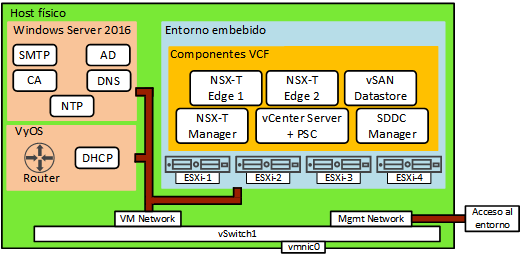
\includegraphics[width=0.6\textwidth]{imaxes/pruebaconcepto/hostFisico.png}
      \caption{Muestra la estructura generada por el instalador VLC. Cuatro hosts ESXi embebidos con los componentes de VMware Cloud Foundation cuyo tráfico circula a través del \textit{port group} VM Network.}
      \label{fig:estructura-generada-por-VLC}
    \end{figure}
    \FloatBarrier

    \begin{figure}[h]
      \centering
      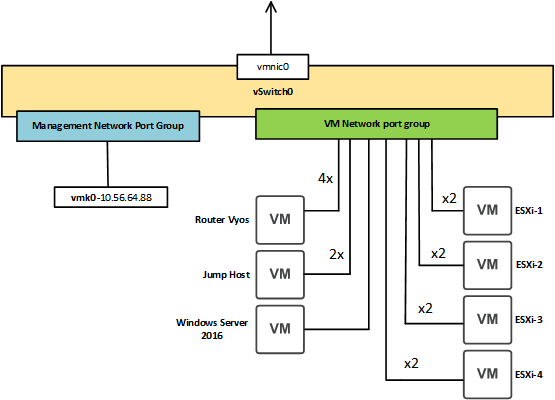
\includegraphics[width=0.6\textwidth]{imaxes/pruebaconcepto/vSwitch0HostFisico.png}
      \caption{Máquinas virtuales en el host físico.}
      \label{fig:VMs-alojadas-host-fisico}
    \end{figure}
    \FloatBarrier

    En la imagen anterior se muestran las VMs que están funcionando sobre el host físico y que representan los componentes de la infraestructura física de un SDDC real, junto con el número de interfaces que se utilizan en cada una. Cada host ESXi generado por VLC cuenta con dos interfaces de red. El router VyOS, Jump Host y Windows Server 2016 se configuran antes del despliegue de VMware Cloud Foundation con VLC y se comunican con el entorno generado por VLC a través del \textit{port group} VM Network. El \textit{port group} Management Network se utiliza para acceder a la configuración del host físico a través de la dirección IP que se indica. Se utiliza la interfaz vmnic0 del host como salida del tráfico generado por el vSwitch0.
    \FloatBarrier

    \begin{figure}[h]
      \centering
      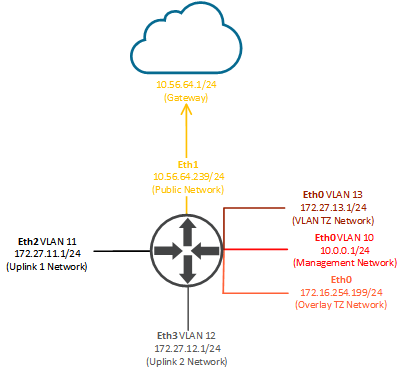
\includegraphics[width=0.4\textwidth]{imaxes/pruebaconcepto/RouterFisicoL3.png}
      \caption{Interfaces del router Vyos.}
      \label{fig:interfaces-router-fisico-L3}
    \end{figure}
    \FloatBarrier

    En la imagen anterior se muestra la configuración del router VyOS. Cada una de las interfaces se debe configurar antes del despliegue de VCF. Todas usan MTU de 8940 Bytes. En las interfaces Eth2 y Eth3 el router utiliza enrutamiento dinámico BGP donde el AS local es 65001 y el AS remoto es AS 65003, configurado para anunciar a sus vecinos la red 10.0.0.0/24 Management Network. Las direcciones configuradas como \textit{neighbour} son: 172.27.11.2, 172.27.11.3, 172.27.12.2 y 172.27.12.3. En la dirección IP 172.27.254.199 de la interfaz eth0, el router proporciona un servidor DHCP que asigna direcciones IP en el rango 172.16.254.0 - 172.16.254.100.
    \FloatBarrier

    \begin{figure}[h]
      \centering
      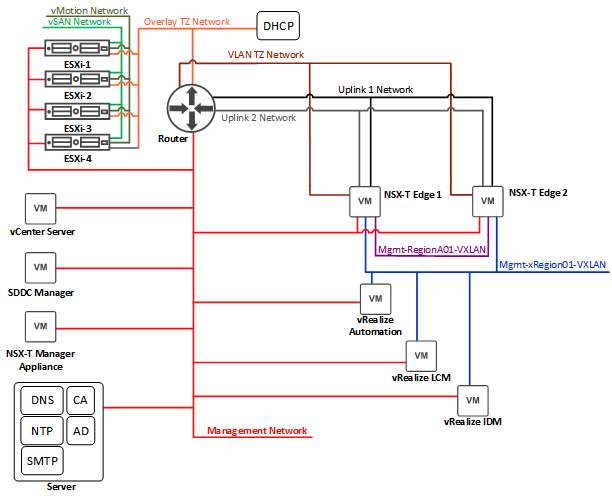
\includegraphics[width=0.6\textwidth]{imaxes/pruebaconcepto/RedDesdeDentro.png}
      \caption{Topología de las redes del entorno desplegado.}
      \label{fig:red-L3-infraestructura-fisica}
    \end{figure}
    \FloatBarrier

    En la imagen anterior se muestran todos los componentes de VMware Cloud Foundation desplegados por VLC y los desplegados posteriormente para completar los objetivos del proyecto, como se conectan con los distintos servicios de red y a que redes se conectan. Las redes Mgmt-xRegion01-VXLAN y Mgmt-Region01A-VXLAN se corresponden a redes virtuales gestionadas por VMware NSX-T que no requieren ninguna configuración adicional en la capa 3 de la infraestructura física (esto se verá con detalle en el apartado de diseño de VMWare NSX-T).
    \FloatBarrier
  \end{subsubsection}
  
\end{subsection}
    %%%%%DISEÑO ARQ. VIRTUAL
\begin{subsection}{Diseño y configuración del Management Domain}
    
    % Esta capa virtual provee infraestructura de almacenamiento, red y cómputo definida por software a través de servicios. En el modelo de despliegue consolidado de VMware Cloud Foundation, todos sus servicios y componentes se encuentran dentro de un mismo cluster (solo una AZ) dentro de la infraestructura, mientras que en el modelo estándar los servicios y componentes de gestión de la infraestructura están situados en clusters distintos (pueden estar en AZ distintas), todos sus componentes se encuentran agrupados en un mismo cluster.
    
    
    
    \subsubsection{Diseño de VMware vCenter Server}
    El componente VMware vCenter Server es el punto de acceso y de control de todas las máquinas virtuales localizados en los hosts ESXi que forman parte de su dominio. En el entorno desplegado se utiliza una instancia de VMware vCenter Server para controlar el \textit{management domain}, se denomina \textit{vcenter-mgmt}. Esta instancia de vCenter Server contiene un dominio que con un cluster vSphere formado por los cuatro hosts ESXi desplegados por VLC, estos se denominan respectivamente \textit{esxi-1}, \textit{esxi-2}, \textit{esxi-3} y \textit{esxi-4}. En vCenter Server se gestionan los recursos de las VMs de cada componente, se monitorizan los recursos, permite la creación y asignación de roles, permisos y usuarios, aisla las redes que usan los recursos que controla de otras instancias de vCenter Server, permite gestionar los grupos de discos de almacenamiento de cada host ESXi que forman el \textit{datastore} de VMware vSAN, administrar las redes a las que se conecta cada componente, en definitiva, VMware vCenter Server es el punto desde el cual se controlan los recursos que utiliza cada componente. Además, incluye el componente PSC que controla el dominio de autenticación de VMware vSphere SSO Domain denominado \textit{local}. Desde vCenter Server también se controlan las características de alta disponibilidad y recuperación ante fallos de VMware vSphere como se verá a continuación. El acceso a vCenter Server se hace a través del componente web vSphere Client.
    \begin{figure}[h]
      \centering
      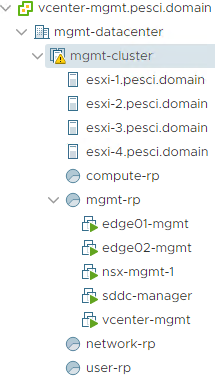
\includegraphics[width=0.2\textwidth]{imaxes/pruebaconcepto/clusterVCenterServer.png}
      \caption{Dominio y cluster vSphere del \textit{management domain}.}
      \label{fig:cluster-vCenter-Server}
    \end{figure}
    \FloatBarrier
    En la imagen anterior se muestra el dominio (\textit{vcenter-mgmt.pesci.domain}) de la instancia de vCenter Server y el cluster vSphere (\textit{mgmt-cluster}) donde se alojan los componentes del \textit{management domain}. Incluye cuatro hosts ESXi y cuatro \textit{resource pools}, uno de ellos contiene las VMs de los componentes dedicados a este \textit{management domain}.
    %  Con vCenter Server se simplifica la escalabilidad del SDDC, la gestión de actualizaciones para los componentes es más sencilla, permite determinar roles específicos y responsabilidades y permite aislar las redes de otras instancias de vCenter Server. Además, para gestionar vSpehere SSO Domain, VMware vCenter Server contiene embebido el componente PSC con todos los servicios necesarios. 
    %  En caso de que existan varios \textit{Workload Domain} se puede habilitar el modo \textit{Enhanced Linked Mode} para poder gestionar todas las instancias de vCenter Server de forma centralizada desde un único vSphere Client.
    % Por lo anterior, en el \textit{management domain} se despliega una instancia de VMware vCenter Server que incluye un cluster de VMware vSphere.
    
    \begin{subsubsection}{Diseño almacenamiento VMware vSAN}
      El almacenamiento del \textit{management domain} desplegado, está implementado con VMwware vSAN. Los cuatro hosts ESXi contienen cuatro grupos de discos cada uno con configuración All-Flash. Como hay cuatro hosts participantes, soporta el fallo de un host lo cual permite dejar hosts fuera de servicio para tareas de mantenimiento. Esto es posible gracias a que con FTT (\textit{Failures-To-Tolerate}) igual a 1 se mantiene la redundancia de los datos almacenados en el \textit{datasotore}, en uno de los hosts. Cada grupo de discos cuenta con cuatro discos uno de ellos para caché, 16 discos en total. Para hacer disponible este servicio de almacenamiento, todos los hosts deben estar conectados a la subred generada para VMware vSAN y utilizar una VLAN para separar su tráfico.
    \end{subsubsection}
        
    \begin{subsubsection}{Diseño cluster VMware vSphere}
    Dentro de un \textit{workload domain} pueden existir varios clusters vSphere con diferentes características según su finalidad. Los hosts ESXi que lo forman pueden ser de diferentes tamaños teniendo en cuenta que se pueden usar menos hosts ESXi de mayor capacidad o más hosts con menores prestaciones, el coste de cada host ESXi, el uso que se le va a dar al cluster y las características máximas y mínimas del cluster vSphere. Para el \textit{management domain} se utiliza un único cluster vSphere con de 4 hosts de los cuales se reserva un host para proveer redundancia. Todos los hosts ESXi cuenta con 64GB de memoria RAM menos uno que tiene 32 GB, y 19.9GHz de CPU. Dentro del cluster hay que configurar los servicios vSphere HA y vSphere DRS para proteger los componentes del SDDC. La configuración que se establece en el \textit{management domain} es la siguiente:
    % En caso de que el \textit{management domain} esté extendido en dos AZ entonces se requieren 4 hosts en cada AZ para proporcionar redundancia y disponibilidad en caso de caída de una de las AZ.
   
    \begin{itemize}
        \item \textbf{vSphere High Availability}: en este servicio la propiedad \textit{Admission Control Policy} permite establecer la cantidad recursos reservados en caso de fallo y como se establece el cálculo de esos recursos. En el \textit{management domain} se configura para el fallo de al menos un host y reserva de recursos según un porcentaje, reservando así el 25\% de la CPU y el 30\% de la memoria RAM ya que funciona mejor cuando las VM usan mucha CPU y memoria. La otra propiedad que se debe habilitar para el correcto funcionamiento del servicio es \textit{VM and Application Monitoring}, que se encarga de reiniciar las VM en caso de caída.
        % que puede ser según el número hosts que pueden fallar en el cluster, según un porcentaje de reserva de rescursos o especificando el host donde se recolocan las VM del host caído.  RAM.  
        \item \textbf{vSphere DRS}: este servicio permite migrar VMs de un host ESXi a otro dentro del mismo cluster vSphere para equilibrar la carga de trabajo y mantener las VMs activas en caso de caída de alguno de los hosts. se activa usando la opción por defecto \textit{Fully Automated} ya que aporta el mejor balance entre consumo de recursos y migraciones de VM innecesarias. Adicionalmente se pueden establecer reglas para determinar reglas de orden de encendido sobre grupos de VM. 
        %En caso de que exista más de una AZ, se deben crear grupos de VM y de hosts de cada AZ para luego implementar reglas de afinidad para que las VM de una AZ no sean migradas a otra AZ ya que esto puede afectar al rendimiento de la VM. 
    \end{itemize}
    % En el modelo consolidado se debe crear un único cluster con un mínimo de cuatro hosts ESXi ya que uno de los hosts se utiliza para asegurar la disponibilidad del almacenamiento vSAN cuando hay algún host inactivo. Este modelo proporciona capacidad de un único fallo por cluster.
    \end{subsubsection}
    \subsubsection{Diseño de red para el cluster vSphere}
    Si bien en VMware Cloud Foundation existe VMware NSX-T, un componente dedicado únicamente a la administración de la red del SDDC, es desde VMware vSphere dónde se encuentran los elementos para establecer redes que separen cada tipo de tráfico de los componentes del SDDC. Estas redes se configuran en base a los siguientes aspectos:
    \begin{itemize}
        \item Separar el tráfico de cada servicio para mejorar la eficiencia de la red y la seguridad. Así se puede ajustar las características de cada red, como el ancho de banda o la latencia, a las necesidades de cada servicio.
        \item Utilizar un único vSphere Distributed Switch por cluster donde se añade un \textit{port groups} por cada servicio.
        % \item Mejorar el rendimiento usando NICs de tipo VMXNET3 en las máquinas virtuales.
        \item Las NICs físicas de cada host ESXi conectados a un mismo vSphere Distributed Switch están conectadas también a la misma red física.
        % \item Aquellas redes que se dedican a servicios de la infraestructura deben estar configuradas con puertos tipo \textit{vmkernel}.
    \end{itemize}
    Para el \textit{management domain} del SDDC se crea un único vSphere Distributed Switch llamado \textit{sddc-vds01} con la siguiente configuración:
    \begin{itemize}
        
        \item Se establece un MTU igual 9000 Bytes para permitir el tráfico de \textit{jumbo frames} ya que son requeridos por algunos de los servicios.
        
        \item Se habilita el servicio \textit{Network I/O} que permite establecer un nivel de prioridad a cada tipo de tráfico. Esto se realiza estableciendo limites de ancho de banda, políticas de balanceo de carga y reserva de recursos para un tipo de tráfico asociado a un servicio. Por cada tipo de tráfico hay cuatro aspectos que se pueden configurar que son \textit{Shares} (indica el \% de ancho de banda que se le da a un tipo de tráfico, el tipo de tráfico que tenga un mayor valor en \textit{Shares} tendrá más prioridad a la hora de usar los recursos), \textit{Reservation} (indica el valor de ancho de banda que se reserva para el tipo de tráfico) y \textit{Limit} (establece un valor máximo para el ancho de banda de un tipo de tráfico). En el \textit{management domain} los tipos de tráfico más relevantes que se deben configurar son los siguientes:
        \begin{itemize}
          \item \textit{Management Traffic}: el valor \textit{Shares} se establece al 50\% (\textit{Normal}) lo cual le da mayor prioridad que el resto de tipos. El resto de valores no se modifican.
          \item \textit{vSphere vMotion Traffic}: el valor \textit{Shares} se establece al 25\% (\textit{Low}) ya que durante el estado normal del entorno este tipo de tráfico no es muy importante. El resto de valores no se modifican.
          \item \textit{vSAN Traffic}: el valor \textit{Shares} se establece al 100\% (\textit{High}) para garantizar que este servicio recibe la cantidad de ancho de banda que necesita. El resto de valores no se modifican.
          \item \textit{Virtual Machine Traffic}: el valor \textit{Shares} se establece al 100\% (\textit{High}) para garantizar que las VMs siempre tienen acceso a la red ya que son una parte importante del SDDC. El resto de valores no se modifican.
        \end{itemize}
        
        \item Para detectar errores de compatibilidad entre la configuración del vSphere Distributed Switch y la red física se habilita el servicio \textit{Health Check}. Este se encarga de comprobar si la configuración de cada VLAN y MTU se adapta a la configuración de la capa física.
        
        \item Como puertos de salida \textit{Uplink} se configuran las interfaces físicas \textit{vmnic0} y \textit{vmnic1}. Como vDS es un componente distribuído, en cada host se usarán ambas interfaces de red como \textit{uplinks}.
        
    \end{itemize}
    En este vSpehere Distributed Switch para el \textit{management domain} se configuran los siguientes \textit{port groups}, que son de tipo \textit{Distributed port group} y de tipo \textit{Uplink port group}:
    \begin{itemize}
           
            \item \textbf{Management port group}: es un \textit{Distributed port group} que comunica a todos los hosts ESXi entre si y transmite el tráfico entre los diferentes componentes de VMware Cloud Foundation, es decir, por este \textit{port group} circulan los comandos de configuración y gestión que los componentes del SDDC se envían entre ellos. Con el nombre \textit{sddc-vds01-mgmt}, en él están configurados los cuatro hosts ESXi y las VMs \textit{vcenter-mgmt}, \textit{sddc-manager}, \textit{nsx-mgmt-1},\textit{edge01-mgmt} y \textit{edge02-mgmt} bajo la subred con IP 10.0.0.0, con máscara de red 255.255.255.0, con VLAN 10 y con MTU igual a 1500 Bytes. Esta red debe ser configurada también en la infraestructura física.
            
            \item \textbf{vMotion port group}: es un \textit{Distributed port group} que está dedicado al tráfico del componente vSphere vMotion para realizar las migraciones de máquinas virtuales de un host a otro. Con el nombre \textit{sddc-vds01-vmotion}, en él están configurados los 4 hosts bajo la subred con IP 10.0.4.0, con máscara de red 255.255.255.0, con VLAN 10 y con MTU igual a 8940 Bytes.
            
            \item \textbf{vSAN port group}: es un \textit{Distributed port group} que está dedicado al servicio de almacenamiento VMware vSAN y por él los hosts acceden al almacenamiento del SDDC. Con el nombre \textit{sddc-vds01-vsan}, en él están configurados los 4 hosts bajo la subred con IP 10.0.8.0, con máscara de red 255.255.255.0, con VLAN 10 y con MTU igual a 8940 Bytes.
            
            \item \textbf{Edge Uplink port group}: es un \textit{Distributed port group} dedicado a las conexiones del component NSX-T Edge que se dedica a dar acceso a determinados servicios y para proporcionar a otros \textit{workload domain} conexión con la red externa. Están gestionados por VMware NSX-T ya que dan servicio a sus componentes. En el entorno existen dos \textit{port groups} para proporcionar redundancia y alta dispobilidad, uno llamado \textit{sddc-edge-uplink01} cuyas instancias están configuradas bajo la red con IP 172.27.11.0 y con máscara de red 255.255.255.0, y otro llamado \textit{sddc-edge-uplink02} cuyas instancias están configuradas bajo la red con IP 172.27.12.0 y máscara de red 255.255.255.0. Ambos \textit{port groups} están configurados como VLAN Trunk (por ellos puede circular tráfico de cualquier VLAN) y tienen un MTU de 8940 Bytes. En los dos están configuradas dos VM llamadas \textit{edge01-mgmt} y \textit{edge02-mgmt}. Estas dos redes también se deben configurar en la infraestructura física.
            
            \item \textbf{Uplink port group}: se trata de un \textit{Uplink port group} al que se le asignan las NICs físicas de cada host para establecer políticas sobre el tráfico que se dirige desde los hosts y VMs hacia fuera del vSphere Distributed Switch. Con el nombre \textit{sddc-vds01-DVUplinks-10}, en él están configuradas las dos NICs físicas de cada host, cada una en una interfaz \textit{uplink}.
            
    \end{itemize}
    \begin{figure}[h]
      \centering
      \includegraphics[width=0.4\textwidth]{imaxes/pruebaconcepto/distributedSwitchEntornoFinal.png}
      \caption{Contenido de vSphere Distributed Switch \textit{sddc-vds01}.}
      \label{fig:port-groups-vSwitch-vSphere}
    \end{figure}
    \FloatBarrier
    En la imagen anterior se muestran todos los \textit{Distributed Port Groups} y \textit{Uplink port group} que se alojan en el vSphere Distributed Switch (\textit{sddc-vds01}) dedicado al \textit{management domain}. En el \textit{port group} \textit{sddc-vds01-DVUplinks-10} se muestra como a cada interfaz \textit{uplink} se mapea una interfaz física (vmnic) de cada host ESXi. Los \textit{port groups} \textit{mgmt-Region01A-VXLAN}, \textit{mgmt-xRegion01-VXLAN} y \textit{sddc-host-overlay} son generados y administrados por el componente VMware NSX-T como se explicará más adelante. Cada \textit{port group} informa de cuantas VMs y hosts ESXi tiene conectados.

    La configuración que se aplica a cada \textit{Distributed port group} descrito anteriormente es la siguiente:
    \begin{itemize}
      \item \textit{Port binding}: permite indidcar como se gestionan los puertos de un \textit{port group} cuando se añade o elimina una VM. Tiene dos opciones de configuración, la primera se denomina \textit{Static Port Binding} y su función consiste en asignar un puerto dentro del \textit{port group} a la VM que se conecta y solo se elimina cuando la VM es borrada. La segunda opción se denomina \textit{Ephemeral Port Binding} y consiste en que el puerto se asigna a la VM cuando esta se enciende y se elimina cuando se apaga o elimina. Para los \textit{port groups} \textit{sddc-vds01-vsan} y \textit{sddc-vds01-vmotion} se configura la opción \textit{Static Port Binding} ya que así se asegura que las VMs se conectan siempre al mismo puerto lo cual permite mantener datos históricos y hacer monitoreo a nivel de puerto. Para los \textit{port group} \textit{sddc-vds01-mgmt}, \textit{sddc-edge-uplink01} y \textit{sddc-edge-uplink02} se configura la opción \textit{Ephemeral Port Binding} ya que como el tráfico que circula por ellos es el que gestiona todos los componentes y da acceso a otras redes etonces se elimina la dependencia del estado de vCenter Server permitiendo que la comunicación continúe aunque vCenter Server no se encuentre operativo.
    
      \item \textit{Load Balancing}: indica como se distribuye el tráfico de salida de cada VM/host que se encuentran en el \textit{port group} entre las NICs físicas. Se selecciona \textit{Route based on physical NIC load}, es decir, el tráfico de una VM se transmite por una única NIC por lo que si esa NIC física está saturada, se asignará otra NIC física a la VM.
      
      \item \textit{Network failure detection}: esta opción permite establecer como debe determinar el \textit{port group} que alguna de las NICs físicas está fuera de servicio. Se selecciona \textit{Link status only} para que esto se determine según el estado que le transmite la NIC física, así se pueden detectar los fallos que ocurren en la red física.
      
      \item \textit{Notify switches}: se habilita para permitir a los host enviar \textit{frames} a los switches físicos para que estos conozcan la localización de las VM que están funcionando en cada host.
      
      \item \textit{Failback}: permite determinar como se reactiva una NIC cuando esta se recupera de un fallo. Se habilita para establecer que la NIC se marcará como activa inmediatamente después de que se haya recuperado. Esta opción se debería desactivar en caso de que el estado de la NIC sea inestable.
      
      \item \textit{Failover Order}: permite determinar que uplinks se deben utilizar, los que se seleccionan como \textit{active} son los que se utilizarán por defecto, los que se seleccionan como \textit{stand by} se usarán cuando los uplinks marcados como \textit{active} se encuentren desactivados. Se seleccionan las dos interfaces \textit{uplink} disponibles en el estado \textit{active}. Para el \textit{port group} \textit{sddc-edge-uplink01} se selecciona la interfaz \textit{uplink1} como activa y se deja sin usar la interfaz \textit{uplink2}, mientras que se configura de forma contraria en el \textit{port group} \textit{sddc-edge-uplink02}.
    \end{itemize}
    
    
    %%%%%%%%%%%%%%%%%%%%%%%%%%%%%%%%%%%%%%%%%%%%
    \subsubsection{Diseño de la red del SDDC con VMware NSX-T}
    En un SDDC debe existir una red virtual, es decir, definida por software o también conocida como \textit{Software-Defined Network}. Esta red al estar construída con componentes de software, se desacopla de la red física sobre la que funciona lo que hace posible que se pueda modificar sin necesidad de cambiar la configuración en la capa física, reduciendo así la complejidad de la red física y el tiempo dedicado a la gestión de la misma. Además, este tipo de arquitectura habilita la posibilidad de implementar múltiples configuraciones de red en tiempo reducido proporcionando elasticidad y flexibilidad a la hora de administrar los recursos, tanto para el administrador como para el usuario final.
    El componente encargado de crear, configurar y administrar la red virtualizada del SDDC es VMware NSX-T que a su vez contiene otros componentes entre los que se dividen distintas responsabilidades y funciones, ya descritos anteriormente.
    
    %%%%% 1 - EXPLICACION DE LOS COMPONENTES DE NSX Y LOS QUE HAY EN EL ENTORNO
    %%%%% 2 - COMO SE DEBE CONFIGURAR LA CAPA FÍSICA Y COMO ESTÁ IMPLEMENTADA EN EL ENTORNO ( parte de esto ya está definido en la parte de red física, REVISAR) => Meter la descripción de lo físico con el resto (modificar ese apartado) [https://docs.vmware.com/en/VMware-Validated-Design/6.0/sddc-architecture-and-design-for-the-management-domain/GUID-C924E896-D9C4-47BF-91D5-DF72605EF63E.html]
    %%%%% 3 - REDES QUE HAY Y COMO SE EXTIENDEN ENTRE AZs
    %%%%% 4 - COMO FUNCIONAN LAS COMUNICACIONES (GENEVE, ROUTING ...)
    
    % En esta sección se describe como VMware Cloud Foundation abstrae la red física en un conjunto de recursos virtuales de red, utilizando los servicios de VMware NSX para crear una capa virtual independiente de la infraestructura física.
    Aunque se recomienda desplegar tres instancias de NSX-T Manager en el \textit{management domain}, VLC solo despliega una única instancia llamada \textit{nsx-mgmt-1} para mejorar el rendimiento del entorno. Además, VLC también genera dos instancias de NSX-T Edge que se denominan \textit{edge01-mgmt} y \textit{edge02-mgmt}. %cada conjunto de instancias de cada componente forman un cluster donde cada VM está protegida por las funcionalidades vSphere HA y vSphere DRS para proveer alta disponibilidad del servicio y migrar las VMs a otra ubicación en caso de caída de una AZ o de un host. 
    Estas VMs están conectadas al \textit{port group} \textit{sddc-vds01-mgmt} que les permite comunicarse entre ellas y con vCenter Server, además las instancias de NSX-T Edge también están conectadas a otros dos \textit{Distributed port group} llamados \textit{sddc-edge-uplink01} y \textit{sddc-edge-uplink02}. %Si existe más de una AZ, varios de los \textit{distributed port groups} se deben extender al resto de AZs para que en caso de que la primera AZ falle sus VMs se puedan migrar a otra AZ y sigan teniendo conectividad. Los \textit{port groups} que deberían estar extendidos en todas las AZ son el \textit{port group} \textit{sddc-vds01-mgmt} de cada AZ\footnote{Cada AZ tiene su propio \textit{Management port group}, entonces en cada AZ debe ser accesible el \textit{Management port group} del resto de AZs.}, los \textit{port group} \textit{sddc-edge-uplink01}, \textit{sddc-edge-uplink02} y \textit{port group} \textit{Edge Overlay}.
    
    Los elementos que utiliza VMware NSX-T para crear una red independiente de la configuración de la red física son \textit{Segment} y \textit{Transport Zone}. Con estos componentes VMware NSX-T puede crear túneles que definen redes de capa 2 sin necesidad de realizar ningún cambio en la configuración de la red física.
    \begin{itemize}
      \item \textbf{Transport Zone} (TZ): define el alcance de la red virtual. Pueden ser de dos tipos distintos, basada en VLAN o basada en Overlay. Una TZ se puede asignar a varios TN que tendrán acceso a los \textit{segments} que funcionen en esa TZ. Un TN se conecta a una TZ a través de un N-VDS los cuales pueden pueden estar conectados a varias TZ de tipo VLAN pero solo a una TZ de tipo Overlay al mismo tiempo.
      
      \item \textbf{Segment}: también llamado \textit{Logical Switch}, representa un dominio de broadcast de capa 2 que forma parte de una \textit{Transport Zone}. El tipo de tráfico puede ser VLAN u Overlay dependiendo de como se haya configurado la \textit{Transport Zone} de la que forma parte. Las VMs de cada TN se pueden conectar a los \textit{Segments} situados en las \textit{Transport Zones} a las que el host está conectado. Estas VMs se pueden comunicar con el resto de VMs conectadas al mismo \textit{Segment}.
       
    \end{itemize}
    Para gestionar las conexiones de cada TN, tanto para los nodos NSX-T Edge como para los hosts ESXi, VMware NSX-T introduce el componente llamado \textbf{NSX-T Virtual Distributed Switch} (N-VDS). Cada TN del \textit{management domain} posee un N-VDS, este elemento conecta sus interfaces a los \textit{segments} que se configuran en cada TN. Para el \textit{management domain} del entorno, VLC despliega dos \textit{transport zones} diferentes.
    \begin{figure}[h]
      \centering
      \includegraphics[width=1\textwidth]{imaxes/pruebaconcepto/OverlayTZSegments.png}
      \caption{\textit{Segments} de la \textit{transport zone} \textit{mgmt-domain-m01-overlay-tz}}
      \label{fig:overlay-TZ-segments-NSXT}
    \end{figure}
    \FloatBarrier
    En la imagen anterior se muestra la \textit{transport zone} con el nombre \textit{mgmt-domain-m01-overlay-tz} de tipo Overlay. Está extendida en los seis TNs que hay en el \textit{management domain} y contiene tres \textit{segments}. El \textit{segment} \textit{mgmt-xRegion01-VXLAN} se utiliza para desplegar aplicaciones que deben ser accesibles desde todas las \textit{regions} que existan en el SDDC, es decir, la misma instancia de una aplicación está disponible desde varios puntos, así se reduce el consumo de recursos y aumenta la disponibilidad de esas aplicaciones ya que pueden migrar a distintas localizaciones según el estado de los recursos. El \textit{segment} \textit{mgmt-Region01A-VXLAN} tiene como finalidad alojar aplicaciones solo deben ser accesibles desde dentro de una misma \textit{region}. En estos dos \textit{segments} es donde se colocan los productos de VMware vRealize. Por último, el \textit{segment} \textit{sddc-host-overlay} es utilizado por los componentes de VMware NSX-T para comunicarse con y entre los diferentes TNs. VMware NSX-T genera en el vSphere vSwitch un \textit{port group} por cada \textit{segment} para poder conectar la VM de cada componente al \textit{port group} que le corresponda.

    \begin{figure}[h]
      \centering
      \includegraphics[width=1\textwidth]{imaxes/pruebaconcepto/VLANTZSegments.png}
       \caption{\textit{Segments} de la  \textit{transport zone} \textit{sfo01-m01-edge-uplink-tz}}
      \label{fig:VLAN-TZ-segments-NSXT}
    \end{figure}
    \FloatBarrier
    En la imagen anterior se muestra la\textit{transport zone} con el nombre \textit{sfo01-m01-edge-uplink-tz} de tipo VLAN. Está extendida en los dos TNs \textit{edge01-mgmt} y \textit{edge02-mgmt} y contiene dos \textit{segments}. Ambos \textit{segments} \textit{VCF-edge-mgmt-cluster-segment-11} y \textit{VCF-edge-mgmt-cluster-segment-12} son utilizados por las instancias de NSX-T Edge para transmitir el tráfico que proviene de los \textit{segments} donde se despliegan aplicaciones hacia la red externa (esto se explicará con más detalle). Estos \textit{segments} utilizan los \textit{port groups} \textit{trunk} del vSphere Switch para transmitir su tráfico hacia las interfaces de red físicas de cada host.
    %\begin{itemize}
      % \item \textit{mgmt-domain-m01-overlay-tz}:
      %   \begin{itemize}
      %     \item Tipo: Overlay
      %     \item Transport Nodes: \textit{edge01-mgmt}, \textit{edge02-mgmt}, \textit{esxi1}, \textit{esxi2}, \textit{esxi3} y \textit{esxi4}.
      %     \item Segments:
      %       \begin{itemize}
      %         \item \textit{mgmt-xRegion01-VXLAN}:
      %           \begin{itemize}
      %             \item VNI: 68589
      %             \item Subred: 10.60.0.0/24
      %             \item VMs: \textit{vrlcm} (10.60.0.60), \textit{vridm} (10.60.0.30)
      %             \item Descripción: se usa para desplegar las aplicaciones (algunos productos de VMware vRealize Suite lo utilizan) que deben ser accesibles desde todas las \textit{Regions} del SDDC, por lo tanto este \textit{segment} debe estar extendido en todo el entorno para que las VMs que se alojen en él puedan mantener la misma configuración de red independientemente del lugar físico donde se encuentren.
      %           \end{itemize}
      %         \item \textit{mgmt-Region01A-VXLAN}:
      %           \begin{itemize}
      %             \item VNI: 67588
      %             \item Subred: 10.50.0.0/24
      %             \item Descripción: su finalidad es alojar aplicaciones que sean accesibles desde una misma \textit{Region}. El alcance de estas aplicaciones está limitado a una \textit{Region} por lo tanto este \textit{segment} solo está extendido dentro de la misma.
      %           \end{itemize}
      %         \item \textit{sddc-host-overlay}:
      %           \begin{itemize}
      %             \item VNI: 67534
      %             \item Descripción: \textit{segment} usado por los componentes de VMware NSX-T para comunicarse entre los diferentes hosts ESXi.
      %           \end{itemize}
      %       \end{itemize}
      %   \end{itemize}
    %   \item \textit{sfo01-m01-edge-uplink-tz}:
    %     \begin{itemize}
    %       \item Tipo: VLAN
    %       \item Transport Nodes: \textit{edge01-mgmt} y \textit{edge02-mgmt}.
    %       \item Segments:
    %         \begin{itemize}
              
    %           \item \textit{VCF-edge-mgmt-cluster-segment-11}:
    %             \begin{itemize}
    %               \item VLAN: 11
    %               \item VMs: \textit{edge01-mgmt} (172.27.11.2/24) y \textit{edge02-mgmt} (172.27.11.3/24).
    %               \item Descripción: usado para transmitir el tráfico saliente hacia la red física.
    %             \end{itemize}
    %           \item \textit{VCF-edge-mgmt-cluster-segment-12}:
    %             \begin{itemize}
    %               \item VLAN: 12
    %               \item VMs: \textit{edge01-mgmt} (172.27.12.2/24) y \textit{edge02-mgmt} (172.27.12.3/24).
    %               \item Descripción: usado para transmitir el tráfico saliente hacia la red física.
    %             \end{itemize}
    %         \end{itemize}
    %       \end{itemize}
    % \end{itemize}
    
    Las TZ, tanto las basadas en Overlay como las basadas en VLAN, sirven para comunicar TNs que se encuentran en distintas partes de la infraestructura física (por ejemplo, en distintos racks) como si estuvieran situadas en el mismo dominio broadcast de capa 2 físico. 
    Aquellas que usan Overlay utilizan el protocolo Geneve para crear un túnel entre los puntos de origen y destino por el cual circula el tráfico generado por los \textit{segments} que pertenecen a esa TZ y que debe salir a la red física para alcanzar su destino. El protocolo Geneve añade una cabecera UDP a cada paquete Ethernet que generan los \textit{segments} cuando este sale del TN donde se generó hacia un TN situado en otra red física. La nueva cabecera incorpora un identificador llamado VNI y es único para cada \textit{segment} (cada \textit{segment} tiene su propio identificador VNI). 
    \begin{figure}[h]
      \centering
      \includegraphics[width=1\textwidth]{imaxes/pruebaconcepto/FrameGeneve.png}
      \caption{Cabeceras de un paquete de red encapsulado con Geneve.}
      \label{fig:Frame-Geneve-Segment-NSXT}
    \end{figure}
    \FloatBarrier
    En la imagen anterior se muestran las cabeceras que forman un paquete de red que pertenece a un \textit{segment} cuando este sale de un TN. Cuando el paquete que circula por la red virtual (contiene los datos que se transmiten y la información de las VMs origen y destino) tiene salir a la infraestructura física para alcanzar el destino, el \textit{transport node} añade la cabecera del protocolo Geneve con el identificador VNI correspondiente, una cabecera UDP con un puerto origen y destino establecidos por defecto, una cabecera IP con las direcciones IP origen y destino de los TN que se están comunicando, y una cabecera Ethernet donde se idican las direcciones MAC de los TN origen y destino. Así, dos VMs conectadas al mismo \textit{segment} pero alojadas en TNs de dominios broadcast diferentes, pueden comunicarse de forma transparente como si estuvieran conectadas directamente una con la otra en la misma subred.
    % \begin{figure}[h]
    %   \centering
    %   \includegraphics[width=1\textwidth]{imaxes/pruebaconcepto/FrameExampleGeneve.png}
    %   \caption{Cabeceras de un paquete capturado con el programa Wireshark que utiliza encapsulación Overlay. Contiene un VNI, las direcciones IP de los elementos que se comunican dentro del \textit{segment} y las direcciones IP de los TN que se comunican \textit{}}
    %   \label{fig:Frame-Geneve-Example-NSXT}
    % \end{figure}
    En las TZ de tipo VLAN, tráfico de sus \textit{segments} es encapsulado añadiendo un identificador de VLAN definido en una plantilla \textit{Uplink Policy}\footnote{A las TZ de tipo Overlay no se les aplica ninguna \textit{Uplink Policy}.} que se asigna a la TZ. Se aplica la misma VLAN para encapsular el tráfico de todos los \textit{segments} de una misma TZ de tipo VLAN. Estas plantillas permiten establecer como debe el N-VDS de un TN tratar el tráfico de la \textit{transport zone} a la que se asigna. En cada una se especifican varias \textit{Teaming Policy}, la VLAN que debe usar el N-VDS cuando tiene que enviar el tráfico fuera del TN y el MTU de cada interfaz \textit{uplinks}. Una \textit{Teaming Policy} indica como el N-VDS utiliza los \textit{uplinks} a nivel de \textit{segment} para distribuir el tráfico y conseguir conexiones redundantes y balanceo de la carga, se especifica una \textit{Teaming Policy} por defecto más otras adicionales. Se aplica una \textit{Uplink Policy} a la TZ de tipo VLAN  \textit{sfo01-m01-dge-uplink-tz}.
    %***UPLINKPOLICY**%
    %  Además, en una \textit{Uplink Policy} se define un mapeo con las interfaces \textit{uplink} establecidas en vSphere Distributed Switch (uplink1 y uplink2) para dirigir el tráfico de cada TZ hacia la red física. 
    %Los TNs \textit{edge01-mgmt} y \textit{edge02-mgmt} proporcionan acceso a la red externa a los \textit{segments} de VMware NSX-T, por ello requieren estar conctados a los dos tienen sus interfaces conectadas a los \textit{uplinks} están mapeados con las NICs físicas de cada host ESXi a través de  a los que están ancladas ambas VMs, es decir, un \textit{uplink} está mapeado con una NIC física del host ESXi. 
    %En las TZ de tipo VLAN, se utilizan plantillas .
    \begin{figure}[h]
      \centering
      \includegraphics[width=1\textwidth]{imaxes/pruebaconcepto/UplinkPolicy13.png}
      \caption{\textit{Uplink Policy} configurada para la \textit{transport zone} \textit{sfo01-m01-dge-uplink-tz}.}
      \label{fig:Uplink-Policy-13-NSXT} 
    \end{figure}
    \FloatBarrier
    En la imagen anteriro se muestra la \textit{Uplink Policy} (\textit{uplink-profile-13}) configurada para la TZ \textit{sfo01-m01-dge-uplink-tz}. Se establece la VLAN 13 como Transport VLAN, utilizado para encapsular el tráfico saliente hacia la red física, y MTU de 8940 Bytes para los uplinks. Hay definidas tres \textit{Teaming Policies}, una por defecto (\textit{Default teaming}) que utiliza \textit{Load Balance Source} para hacer un mapeo uno a uno entre las interfaces de cada VM y uno de los \textit{uplinks} (todo el tráfico correspondiente a esa interfaz se envía y recibe por el mismo \textit{uplink}), y dos adicionales \textit{uplink1-named-teaming-policy} y \textit{uplink2-named-teaming-policy} que utilizan \textit{Failover Order} donde se establece un \textit{uplink} como activo por donde se transmite todo el tráfico y otros de reserva que se usan en caso de que el \textit{uplink} activo falle (en una de las políticas todo el tráfico se reenvía por \textit{uplink1} y en la otra por \textit{uplink2}).

    A los \textit{segments} \textit{VCF-edge-mgmt-cluster-segment-11} y \textit{VCF-edge-mgmt-cluster-segment-12} pertenecientes a la TZ \textit{sfo01-m01-dge-uplink-tz} se les asigna la \textit{Teaming Policy} \textit{uplink1-named-teaming-policy} y \textit{uplink2-named-teaming-policy} respectivamente. De esta forma se consigue que el tráfico que circula por cada uno de ellos solo utilice un único \textit{uplink}. 
    \begin{figure}[h]
      \centering
      \includegraphics[width=0.6\textwidth]{imaxes/pruebaconcepto/UplinkDesign.png}
      \caption{Topología de red de las insterfaces \textit{uplink}.}
      \label{fig:Uplink-Design-Edge-NSXT} 
    \end{figure}
    \FloatBarrier
    En la imagen anterior se muestra la topología que forman las instancias de NSX-T Edge para generar la redundancia y alta disponibilidad en las rutas hacia la red externa para las aplicaciones cuya red está gestionada por VMware NSX-T, desde el punto de vista de VMware vSphere. Cada TN Edge posee dos interfaces \textit{uplink} que durante su configuración se mapea cada una con uno de los \textit{trunk port groups} de vSphere Switch. Las interfaces \textit{uplink} que se indican en la \textit{Teaming Policy} se refieren a las de la instancia de NSX-T Edge, no las de vSphere vSwitch, por lo tanto cada uno de los \textit{segments} utiliza solo uno de los \textit{uplinks} que combinado con la configuración de los \textit{port groups} de vSphere vSwitch establecen las rutas que se muestran en la imagen.
    % Así, como cada TN de NSX-T Edge está anclado a dos \textit{trunk port groups} en vSphere Switch por donde se transmite el tráfico de estos dos \textit{segments} y cada uno de esos \textit{segments} transmite por un único \textit{uplink}, se consigue que estas rutas hacia la red externa sean redundantes y con alta disponibilidad para las aplicaciones cuya red está gestionada por VMware NSX-T.
    % Para la TZ de tipo VLAN \textit{sfo01-m01-dge-uplink-tz} se especifica la siguiente \textit{Uplink Policy}:
    % \begin{itemize}
    %   \item Nombre: \textit{uplink-profile-13}
    %   \item Transport VLAN: 13
    %   \item MTU: 8940
    %   \item Teaming Policy: se especifican tres, una por defecto y dos adicionales:
    %     \begin{itemize}
    %       \item \textit{Default teaming}: \textit{Load Balance Source}, hace un mapeo uno a uno entre cada interfaz virtual de cada VM y uno de los \textit{uplinks} del N-VDS, así todo el tráfico correspondiente a esa interfaz se envía y recibe por el mismo \textit{uplink}.
          
    %       \item \textit{uplink1-named-teaming-policy}: \textit{Failover Order}, se establece un \textit{uplink}, \textit{uplink1} en este caso, como activo que se utiliza para enviar todo el tráfico, y una lista de \textit{uplinks} ordenados que se utilizan en caso de que el primero no esté disponible, vacía para esta \textit{Teaming policy}.
    %       \item \textit{uplink2-named-teaming-policy}: \textit{Failover Order}, donde el \textit{uplink} activo es \textit{uplink2} y la lista de \textit{uplinks} de reserva está vacía.
    %     \end{itemize}
    % \end{itemize}
    % A los \textit{segments} de esta TZ, \textit{VCF-edge-mgmt-cluster-segment-11} y \textit{VCF-edge-mgmt-cluster-segment-12} se les asignan las \textit{Teaming Policy} \textit{uplink1-named-teaming-policy} y \textit{uplink2-named-teaming-policy} respectivamente. Con esta configuración el tráfico de cada \textit{segment} circula por una única NIC física del host ESXi. Esto, junto con la configuración \textit{Failover Order} establecida para los \textit{port groups} \textit{sddc-edge-uplink01} y \textit{sddc-edge-uplink02} en el vSphere vDS,se consigue que el tráfico de salida hacia la red física perteneciente a los componentes de VMware NSX-T y todas las aplicaciones cuya red gestiona VMware NSX-T, sea distribuído por dos redes distintas proporcionando redundancia y disponibilidad del servicio en caso de que ocurra una caída de alguna de las conexiones.
    %*****************%

    Esta encapsulación, tanto VLAN como Overlay, tiene lugar cuando los paquetes salen de la interfaz de una VM y entran en el N-VDS del TN. Para ello, cada TN tiene dispositivo llamado \textit{Tunnel End Point} (TEP) al que se le asigna una dirección IP utilizada para enviar y recibir el tráfico entre VMs que se encuentran en el mismo \textit{segment} pero se alojan en TNs situados en redes L2 diferentes\footnote{En el entorno desplegado todos los TN se encuentran dentro de la misma red física. Esto implica que no se genere tráfico con los TEPs ya que todas las TZs funcionan sobre un único dominio broadcast.}. Los TNs que son hosts ESXi obtienen su dirección TEP de un servidor DHCP\footnote{El servidor DHCP hace que se simplifique el proceso de configuración de un nuevo host ESXi ya que le asigna una dirección IP de forma automática.} mientras que los que son instancias de NSX-T Edge la dirección IP se asigna de forma manual. El TEP de cada TN tiene dos direcciones IP asignadas puesto que cada uno tiene dos interfaces de red, \textit{esxi-1} tiene las direcciones 172.16.254.10 y 172.16.254.11, \textit{esxi-2} tiene las direcciones 172.16.254.12 y 172.16.254.13, \textit{esxi-3} tiene las direcciones 172.16.254.14 y 172.16.254.15, \textit{esxi-4} tiene las direcciones 172.16.254.16 y 172.16.254.17, \textit{edge01-mgmt} tiene las direcciones 172.27.13.2 y 172.27.13.3, y \textit{edge02-mgmt} tiene las direcciones 172.27.13.4 y 172.27.13.5.
    
    Al crear un \textit{segment} dentro de una TZ, se configura un modo de replicación que indica como se retransmite el tráfico Broadcast, Multicast y Unknown Unicast propio del \textit{segment} cuando este tiene que viajar a un TN que está en una ubicación distinta en el medio físico. El modo de replicación que se utiliza en todos los \textit{segments} es \textit{Two-Tier Hierarchical Mode}. 
    \begin{figure}[h]
      \centering
      \includegraphics[width=0.6\textwidth]{imaxes/pruebaconcepto/Two-tier-ReplicationMode.png}
      \caption{Modo de replicación \textit{Two-Tier Hierarchical}.}
      \label{fig:Frame-Geneve-Segment-NSXT}
    \end{figure}
    \FloatBarrier
    En la imagen anterior se muestra un ejemplo del funcionamiento del modo de replicación \textit{Two-Tier Hierarchical}. (1) Cuando el TN HV1 envía tráfico BUM a la red primero lo hace a los TNs que están en su mismo dominio, (2) después envía una copia de ese tráfico a un único TN de cada dominio broadcast donde exista el \textit{segment} propietario del tráfico y, finalmente, (3) el TN de cada localización lo retransmite al resto de TNs de su dominio que lo requieran. De este modo se reduce el número de paquetes que el TN origen debe enviar a través de la red física.
    % Este consiste en que cuando desde un TN se envía algún tipo de tráfico BUM de un \textit{segment} cuyos TNs están distribuídos en distintos puntos de la infraestructura física, el TEP del TN origen detecta que debe retransmitir el tráfico a una red externa, en la red externa se selecciona un TN que recibe el tráfico y lo reenvía al resto de TNs dentro del mismo dominio de red que deben recibir ese tráfico, así se reduce . El tráfico solo se enviará a los TN que contienen VMs que forman parte del \textit{segment} que lo genera. Es el componente NSX-T Controller quien se encarga de actualizar e indicar a los TNs toda la información para que esta comunicación sea correcta.
    
    El objetivo es crear nuevas subredes, es decir \textit{segments} que se expanden por los distintos TNs adheridos a la \textit{transport zone} correspondiente, y conectarlas a un router virtual para al final formar subredes distribuidas con servicios de red también	distribuidos y virtualizados, todo gestionado desde VMware NSX-T y sin tener que configurar la red física. Para completar esto, VMware NSX-T introduce routers virtuales que se encuentran embebidos y distribuídos dentro del hypervisor ESXi de cada TN y que proporcionan enrutamiento entre \textit{segments} y servicios de red distribuídos. Permiten definir un \textit{gateway} para cada \textit{segment} a través del cual las VMs conectadas pueden acceder a la red externa y los servicios de red. La herramienta VLC despliega para el \textit{management domain} un modelo de enrutamiento de doble capa (\textit{Two Tier Routing}) donde se utilizan dos routers virtuales, \textit{Tier-0} (\textit{mgmt-domain-tier0-gateway}) dedicado a gestionar el acceso a la red externa a través del router VyOS con conexiones redundantes, y \textit{Tier-1} (\textit{mgmt-domain-tier1-gateway})que gestiona el enrutamiento entre \textit{segments} y proporciona servicios de red a las VMs.

    \begin{figure}[h]
      \centering
      \includegraphics[width=0.5\textwidth]{imaxes/pruebaconcepto/topologiaTwoTierRouting.png}
      \caption{Topología de los routers virtuales de \textit{Tier-1} y \textit{Tier-0}.}
      \label{fig:Topology-TwoTier-Routing-NSXT}
    \end{figure}
    \FloatBarrier
    En la imagen superior se muestra la topología del modelo de dos routers virtuales y los \textit{segments} a los que se conecta cada uno desde el punto de vista de NSX-T. El router de Tier-1 enruta el tráfico entre los \textit{segments} a los que está conectado y hacia el router de Tier-0 que se encarga de transmitir el tráfico hacia la red física.

    Un router router lógico está formado por dos componentes:
    \begin{itemize}
      
      \item \textbf{Distributed Router} (DR): que gestiona el enrutamiento y se a subredes a través de sus interfaces lógicas. Estas subredes pueden ser \textit{segments} u otro DR. A cada interfaz se le asigna una dirección MAC y una dirección IP que representa el \textit{gateway} de la subred. Este componente está distribuído en todos los TN, tanto hosts ESXi como instancias de NSX-T Edge manteniendo la misma configuración (interfaces,tablas de enrutamiento, etc.). Su función es redirigir el tráfico que recibe entre las interfaces que tiene disponibles, es decir, enruta el tráfico entre los diferentes \textit{segments} a los que está conectado el router virtual Tiene una interfaz llamada \textit{Internal transit Link} conectada a la red \textit{Internal Transit Network} que se utiliza para conectar todos los DR y SR de un \text{Tier} distribuídos en los TN.
      
      \item \textbf{Service Router} (SR): proporciona servicios de red de forma centralizada (NAT, DHCP, Load Balancer, VPN, Gateway Firewall y Bridging L2) y proporciona acceso a la red externa. Este componente no está distribuído entre los diferentes TN, solo se se encuentra distribuido en las instancias de NSX-T Edge. Los servicios que proporciona solo se entregan a los recursos cuya red está gestionada por VMware NSX-T. Posee la interfaz \text{Internal Transit Link} para comunicarse con el resto de DR y SR pertenecientes al mismo \text{Tier}, dos interfaces \textit{External Interface} que se conectan a los \text{segments} que dan acceso a la red externa \footnote{La \textit{External Interface} solo existe en \textit{Tier-0} ya que es el router que se comunica con el dispositivo físico.}, la interfaz \textit{Router Link}\footnote{Router Link Network utiliza por defecto la subred 100.64.0.0/16.} que conecta el SR de \textit{Tier-0} con el de \textit{Tier-1}, y la interfaz \textit{Internal transit} que se habilita cuando se activa la opción \textit{Inter SR iBGP}\footnote{Inter SR iBGP Network utiliza por defecto la subred 169.254.0.0/24.} y que comunica los SR de las dos instancias de NSX-T Edge.
    \end{itemize}

    \begin{figure}[h]
      \centering
      \includegraphics[width=0.8\textwidth]{imaxes/pruebaconcepto/EstructuraInternaTiers.png}
      \caption{Estructura interna de los routers virtuales de \textit{Tier-0} y de \textit{Tier-1}.}
      \label{fig:estructura-interna-TwoTier-Routing-NSXT}
    \end{figure}
    \FloatBarrier
    En la imagen superior se muestran los componentes internos de cada router virtual y como estos están distribuidos por todos los TNs. El router \textit{mgmt-domain-tier0-gateway} tiene el componente SR distribuído en dos TN que son las instancias de NSX-T Edge, y el componente DR distribuido en todos los TNs. El SR situado en \textit{edge01-mgmt} está conectado al \textit{segment} \textit{VCF-edge\_mgmt-edge-cluster-segment-11} y usa la dirección IP 172.27.11.2, y otra interfaz conectada al \textit{segment} \textit{VCF-edge\_mgmt-edge-cluster-segment-12} donde usa la IP 172.27.12.2, mientras que el SR de \textit{Tier-0} situado en \textit{edge02-mgmt} se conecta a los mismos \textit{segments} pero usando las direcciones 172.27.11.3 y 172.27.12.3 respectivamente. El router \textit{mgmt-domain-tier1-gateway} tiene el componente SR distribuido en las dos instancias de NSX-T Edge y el componente DR distribuido por en todos los TNs. Ambos SR están conectados con los SR de \textit{Tier-0} para transmitir el tráfico hacia la red física. Los DR de \textit{Tier-1} están conectados a los \textit{segments} \textit{Mgmt-RegionA01-VXLAN} y \textit{Mgmt-xRegion01-VXLAN} para proporcionar enrutamiento y servicios a las VMs situadas en ellos.
    
    La razón de tener dos capas de enrutamiento se debe a la configuración del router \textit{mgmt-domain-tier0-gateway}. En este router se utiliza BGP para comunicarse con el router físico a través de las \textit{external interfaces} (se establece 65003 como \textit{autonomous system} local)\footnote{El uso de BGP simplifica la configuración de nuevas rutas cuando se añaden componentes al entorno, y que no se pierda la conectividad en caso de caída de alguna de las interfaces. Este protocolo también se configura en las interfaces del router Vyos}, la opción \textit{Inter SR iBGP} establecer una comunicación mediante BGP entre las instancias distribuídas del componente SR de \textit{Tier-0} para que se pueda seguir transmitiendo el tráfico en caso de que alguna de las interfaces de una instancia de NSX-T Edge esté fuera de servicio, se activa el protocolo ECMP para balancear el tráfico hacia la red física entre los caminos disponibles ya que en conjunto, en el router de \textit{Tier-0} existen cuatro rutas posibles para alcanzar el router VyOS. Un aspecto importante es la configuración de la disponibilidad de un router virtual ya que determina el modo en el que se va a ejecutar. En el router de \textit{Tier-0} se selecciona el modo \textit{active-active} el cual implica que las dos instancias de SR funcionan ambas de forma activa, es decir, el tráfico que reciba cada una será encaminado por una subred diferente proporcionando así mayor ancho de banda, mayor disponibilidad y mayor escalabilidad. Esto esto último no es compatible con servicios de red centralizados, por ello es necesario desplegar al menos un router lógico de \textit{Tier-1} (\textit{mgmt-domain-tier1-gateway}) configurado con el modo \textit{active-stanby} el cual solo se utiliza una de las dos instancias del SR de \textit{Tier-1} por lo tanto el tráfico dirigido a este router siempre será recogido en un único punto. Así, en el router \textit{mgmt-domain-tier1-gateway} es donde se pueden desplegar servicios de red como NAT, Load Blancing, DNS y VPN, para los \textit{segments} que están conectados.

    \end{subsection}
    
    \begin{subsection}{Operaciones de la Arquitectura}
    El entorno ya está configurado para funcionar como un SDDC, a partir de este punto ya no es necesario realizar ninguna modificación en la infraestructura física ya que todas las tareas que se deben realizar están dentro del alcance de los componentes de VMware Cloud Foundation. Para finalizar la construcción del SDDC y habilitar un servicio donde los usuarios puedan aprovisionar recursos bajo demanda, se instalarán sobre el entorno desplegado las aplicaciones Workspace ONE Access \footnote{VMware vRealize Identity Manager} (WSA) y VMware vRealize Automation (vRA). La primera permite al administrador conectar con el servidor de usuarios Active Directory y gestionarlos para proveer un servicio de autenticación centralizado a múltiples aplicaciones como VMware vRealize Automation. La segunda aplicación permite a los usuarios aprovisionar recursos de forma automatizada desde un catálogo de recursos. VMware vRealize Suite Licfecycle Manager (vRSLCM) es el componente que permite administrar vRA y WSA, su instalación y actualizaciones, las contraseñas de administrador y sus certificados, para ello necesita comunicarse con VMware vCenter Server. Se desplegará una instancia de cada componente en el \textit{management domain} creado anteriormente y estarán conectadas al \textit{segment}/subred \textit{Mgmt-xRegion01-VXLAN}.
    
    % \begin{subsubsection}{vRealize Suite Lifecycle Manager}
        
    % \end{subsubsection}
    \begin{subsubsection}{Workspace One Access}
        Los usuarios que necesiten acceder a vRA deben estar registrados en el directorio de Workspace One Access. Este componente centraliza el acceso de todos los productos de VMware vRealize. Cuando se despliega se debe configurar un Active Directory que en el caso del entorno está situado en la VM con Windows Server 2016. Dentro del Active Directory existen grupos de seguridad y perfiles de usuario, un perfil de usuario contiene información como nombre, apellidos, dirección e-mail, nombre de usuario y contraseña\footnote{Se pueden configurar más campos pero los que se describen son los obligatorios a la hora de crear un usuario.}, y este puede formar parte de varios grupos de seguridad. Una vez configurado, cada aplicación se conectará a WSA y se podrán asignar roles para los grupos de seguridad y usuarios estableciendo así un nivel de acceso. Además, cada usuario registrado tendrá disponible un catálogo de aplicaciones en el portal de WSA cuyo administrador establecerá que aplicaciones están habilitadas para cada usuario o grupo, eso sí, para que el usuario pueda acceder a ella previamente se debe establecer un rol para ese usuario dentro de la aplicación.

        %*****USUARIOS QUE HAY EN EL ENTORNO Y EL ACCESO A CADA APLICACIÓN*******%
        \begin{figure}[h]
            \centering
            \includegraphics[width=0.4\textwidth]{imaxes/vRealize_pruebaconcepto/usuariosDefinidos.png}
            \caption{Muestra los usuarios definidos en el Active Directory sincronizados en Workspace One Access.}
            \label{fig:users-defined-AD}
        \end{figure}
        \FloatBarrier
        En la Figura \ref{fig:users-defined-AD} se muestran los dos usuarios definidos en el Active Directory y dos usuarios que se corresponden a los perfiles de administración de WSA, no se utilizarán grupos de seguridad para reducir la complejidad pero su configuración en las aplicaciones de VMware es igual que para los perfiles de usuario. En un entorno real existen usuarios que controlan a otros usuarios y establecen su nivel de acceso, a parte de los perfiles de administrador de cada aplicación. Para el entorno se define el perfil \textit{adminuser} que será el encargado de gestionar el acceso de dos usuarios (\textit{baseuser1} y \textit{baseuser2}) que serán los que consuman a las aplicaciones desplegadas (vRSLCM y vRA). El primero tendrá acceso y permisos de edición en las aplicaciones vRSLCM y vRA, mientras que los dos usuarios base solo podrán acceder a vRA y dentro de este el usuario admin definirá que servicios están habilitados para cada uno.

        %************************************************************************%

    \end{subsubsection}

    \begin{subsubsection}{VMware vRealize Automation}
        El punto a través del cual los usuarios pueden aprovisionar sus recursos es vRealize Automation. Este producto provee el servicio cloud. 
        \begin{figure}[h]
            \centering
            \includegraphics[width=0.8\textwidth]{imaxes/vRealize_pruebaconcepto/ComponentesVRA.png}
            \caption{Componentes de VMware vRealize Automation y tareas que realiza cada rol de usuario.}
            \label{fig:users-defined-AD}
        \end{figure}
        \FloatBarrier
        Internamente vRA se divide en varios servicios que permiten gestionar los diferentes aspectos de la cloud. Para centrarse en los objetivos de este proyecto solo se hace referencia a dos de esos servicios, el primero es Cloud Assembly el cual permite administrar la infraestructura disponible controlar el uso que se hace de esos recursos, y el segundo es Service Broker, utilizado por los usuarios para aprovisionar los recursos desde un catálogo de plantillas. La obtención de los recursos por parte del usuario se hace desplegando una serie de plantillas llamadas Blueprints diseñadas previamente, en donde se define un conjunto de VMs y recursos de red y de almacenamiento incluyendo otros aspectos como la configuración de cada uno de los recursos, como redes de la infraestructura que se utilizan, cantidad de almacenamiento, o la ubicación del despliegue en la infraestructura. Son ficheros de código con extensión \textit{.yaml} donde se indican etiquetas, aunque también se pueden diseñar con un editor gráfico. Estas plantillas están relacionadas con proyectos, una plantilla pertenece a uno o varios proyectos donde existe un coordinador de proyecto que se encarga de diseñar Blueprints y de administrar los usuarios miembros de ese proyecto. Los proyectos de vRA permiten limitar los recursos para que un conjunto de usuarios pueda desplegar los componentes definidos en las Blueprints disponibles, como la cantidad de memoria RAM, cantidad de instancias que se pueden desplegar y cantidad de almacenamiento, también aquellas redes que se pueden utilizar. Desde el punto de vista de vRA, la infraestructura se divide en Cloud Zones, las cuales son conjuntos de recursos situados en distintos proveedores Cloud que pueden ser públicos como AWS o Azure, o privados que solo pueden ser clusters vSphere. En el caso del entorno desplegado solo se tendrá una única Cloud Zone de tipo vSphere. En cada Cloud Zone se define como se deben distribuir los recursos aprovisionados sobre la infraestructura. 
        Finalmente será el administrador de la infraestructura el que se encargue de proveer los recursos, administrar los proyectos disponibles, gestionar los coordinadores de cada proyecto y controlar y limitar el uso de los recursos.
        % Finalmente, vRA permite configurar tarjetas donde se puede definir el coste del aprovisionamiento de CPU, almacenamiento y memoria RAM, además del coste de uso de otros elementos como sistemas operativos, el uso de una determinada red o el uso de una determinada Cloud Zone. Estas tarjetas se asignan por proyecto para determinar el coste que tendrá el consumo de recursos por mes.


    \end{subsubsection}

    
\end{subsection} 
   
    \end{section}
%\begin{section}{Despliegue de VMware Cloud Foundation}
En esta sección se describe el entorno y los procedimientos llevados a cabo para desplegar VMware Cloud Foundation sobre la infraestructura.
\begin{subsection}{Prueba de concepto}
Para poder realizar la instalación sin afectar al funcionamiento actual del CPD del CITIC, se habilita un entorno aislado. Con esto se evita la aparición de fallos que pueden ser críticos para la infraestructura y a la vez permite explorar esta nueva plataforma sin tener en cuenta los riesgos de hacerlo sobre la infraestructura real.\\
 ************DESCRIPCION DEL ENTORNO (INFRAESTRUCTURA)*********\\
\end{subsection}
\begin{subsection}{Preparación del entorno}
En esta sección se describe la arquitectura y configuración de todos los componentes de la infraestructura del entorno donde se va a realizar el despliegue. Las opciones de configuración se establecen de acuerdo con lo descrito en los apartados anteriores sobre el diseño de la infraestructura y arquitectura de VMware Cloud Foundation.
\\


*********SERVICIOS QUE SE CREAN (CONFIG DNS,DHCP, ROUTER...)***********\\

\subsubsection{VMware Cloud Foundation Builder}
El despliegue de la plataforma VMware Cloud Foundation se realiza través de una \textit{appliance} llamada VMware Cloud Foundation Builder. Esto es una máquina virtual que se instala en el entorno desde una archivo con formato \textit{.ova}, proporcionado por VMware, y que contiene el instalador de VMware Cloud Foundation. Este instalador se encarga de recibir los parámetros de configuración de la infraestructura donde se va a hacer el despliegue, los valida y a continuación despliega el \textit{management domain} del SDDC con todos sus componentes. Cuando termina el proceso, transfiere el inventario y el control del sistema al componente SDDC Manager y VMware Cloud Foundation Builder puede ser eliminado.\\
Esta máquina virtual tiene los siguientes requisitos:
\begin{itemize}
    \item \textbf{CPU}: 4 vCPU.
    \item \textbf{Memoria RAM}: 4 GB.
    \item \textbf{Almacenamiento}: 350 GB.
    \item Acceso al servidor DNS y NTP para validar la configuración de VMware Cloud Foundation.
    \item Acceso a la red \textit{management} para comunicarse con todos los hosts ESXi.
\end{itemize}


*********CLOUD BUILDER*************\\

*********HOJA DE PARÁMETROS********\\
\end{subsection}
\end{section}
%

\section{Despliegue del servicio}
En este apartado se expone el proceso de despliegue de VMware Cloud Foundation sobre el entorno creado específicamente para esto. Se muestran las configuraciones aplicadas y los cambios realizados sobre la infraestructura.

\subsection{Cumplimiento de requisitos}

\subsubsection{Almacenamiento}
Según la documentación de de VMware, el entorno debe tener una \ref{Word:capacidad} de almacenamiento mínima determinada para poder instalar los componentes de Cloud Foundation si se va a crear como mínimo un Management Domain y un VI Domain. La capacidad inicial del entorno es de 2,34TB de almacenamiento, 96 GBde memoria y 4 nodos ESXi, lo cual no es suficiente para cumplir con este requisito.
Además, Cloud Foundation requiere un disco de arranque en cada nodo de 16GB por lo que es necesario aumentar el tamaño de este disco de 8GB a 16GB.


\subsubsection{Redes}
Antes del despliegue es necesario especificar cuatro redes, una dedicada a vSAN, otra para vMotion, otra para la gestión de los componentes y una cuarta red para el tráfico de las máquinas virtuales (Sección \ref{subsubsec:redLogicaCF}). Inicialmente solo falta una red para habilitar el servicio de vMotion, el resto de redes necesarias ya están creadas y configuradas (Sección \ref{sec:redPrueba}). Esta nueva red también debe tener acceso al resto de componentes por lo que hay que añadir un nuevo adaptador de red (NIC) en el servidor externo. Además, también hay que añadir las nuevas rutas entre redes para que el servidor pueda realizar el enrutamiento del tráfico correctamente.\\
******FOTO NUEVOS ADAPTADORES DE RED*****\\
******FOTO NUEVA TABLA DE ENRUTAMIENTO*****\\

En cuanto a la red física, está configurada para aceptar el MTU igual a 1500 lo cual no cumple con el requisito mínimo (Sección \ref{subsubsec:redFisica}). El tráfico etiquetado si que está habilitado en la red física. Como se está trabajando sobre un entorno físico virtualizado entonces se puede modificar de forma sencilla. Además, cada nodo tiene cuatro \ref{Word:vmnic} por lo que cumple con el mínimo de dos NIC por nodo (Sección \ref{subsubsec:domainVI}).

\subsubsection{Servicios internos y externos}
El tráfico de los servicios y puertos especificados [Sec. \ref{subsubsec:servInterno}] deben estar habilitados en el firewall interno de cada nodo y su tráfico está permitido a través de la red. Inicialmente, el tráfico a cada puerto está habilitado desde cualquier dirección IP.\\
Inicialmente, los servicios externos (DNS, DHCP y NTP) están habilitados en un servidor alcanzable por todas las redes configuradas.
\iffalse
Como es necesario habilitar una nueva red para el componente vMotion entonces hay que añadir un nuevo adaptador de red en el servidor para que esta red pueda acceder a los servicios y comunicarse con el resto de componentes.\\
\fi
Durante el proceso de despliegue de Cloud Foundation se instalarán nuevos componentes por lo que también es necesario configurar el DHCP añadiendo más rangos de direcciones IP, y el DNS para que todos los componentes y máquinas virtuales del entorno sean alcanzables desde todas las redes.\\
*****FOTO DE LO QUE SE HA AÑADIDO EN DHCP Y DNS *****\\

\iffalse
Los servicios externos (Sección \ref{subsubsec:servExterno}) se deben habilitar en un servidor alcanzable por cada nodo por lo que al añadir nuevas redes al entorno es necesario incluir más adaptadores de red en la máquina virtual con Windows Server para darles acceso al DNS, al DHCP y a NTP.
\fi
***RESUMEN DE COMO QUEDA ANTES DE EMPEZAR LA INSTALACIÓN CON LOS CAMBIOS REALIZADOS*******


\subsection{Despliegue VMware Cloud Foundation Builder}
Para instalar VMware Cloud Foundation, antes es necesario instalar VMware Cloud Foundation Builder (Sección \ref{subsec:cloudBuilder}). Esta máquina virtual se despliega desde vSphere Client a partir de un archivo \textit{ova} proporcionado por VMware, en este caso la versión que se instalará es \underline{2.2.0.0-14866160}.
Una vez deplegado Cloud Builder y antes de iniciar la instalación de Cloud Foundation, es necesario adjuntar una hoja de parámetros con los datos de configuración que se deben aplicar, tales como el DNS, redes, y credenciales de los componentes que se van a crear posteriormente.

\subsubsection{Configuración de la máquina virtual}

\subsubsection{Hoja de parámetros}
Esta hoja es un archivo \textit{xlsx} de Excel donde se indica la configuración sobre componentes que ya existen en el entorno y los que se van a desplegar. Estos datos permiten a Cloud Builder y SDDC Manager automatizar el proceso de instalación y configuración inicial de los componentes para generar el Management Domain. Estos datos se dividen en varias categorías:
\begin{itemize}
    \item \textbf{\textit{Prerequisite Checklist}}: muestra una lista de comprobaciones a realizar sobre la configuración inicial del entorno antes de iniciar el despliegue.
    \item \textbf{\textit{Management Workloads}}: permite introducir los números de las licencias necesarias para utilizar todos los componentes de VMware Cloud Foundation y una estimación de los recursos necesarios para el Management Domain.
    \item \textbf{\textit{Users and Groups}}: permite indicar las credenciales para cada usuario de cada componente de VMware Cloud Foundation. Estas credenciales deben cumplir un unos requisitos mínimos.
    \item \textbf{\textit{Hosts and Networks}}: en esta categoría se indican las direcciones IP de las redes requeridas y las direcciones IP de cada host ESXi. También se pueden indicar los fingerprint de SSH y thumprints de SSL de cada host ESXi para que estos sean validados antes de conectarse a ellos durante la instalación (esto es opcional).
    \item \textbf{\textit{Deploy Parameters}}\footnote{Todos los nombres y direcciones IP indicados deben estar configuradas en el DNS para que se puedan resolver a través de ese servicio.}: Aquí se indican los detalles de configuración que se van a desplegar. Existen varios apartados\cite{deploysheet}:
        \begin{itemize}
            \item \emph{Existing Infrastructure Details}: se indican los datos de configuración de servicios configurados inicialmente en el entorno. Estos son DNS, NTP, Single Sign-On y el almacén de vSAN.
            
            \item \emph{vSphere Infrastructure}: se indican los nombres y direcciones IP de las máquinas virtuales de los componentes vCenter Server y Platform Services Controller. 
            
            \item \emph{NSX}: se debe indicar las direcciones IP y los nombres de las máquinas virtuales del componente NSX que se van a desplegar.
            
            \item \emph{vRealize Log Insight}: se indican las direcciones IP y nombres de las máquinas virtuales del \textit{Load Balancer} y de los tres nodos de vRealize Log Insight (un nodo \textit{Master} y dos nodos \textit{Workers}).
            
            \item \emph{SDDC Manager}: se indica el nombre de la máquina virtual, la dirección IP y su máscara de red para el componente SDDC Manager.
        \end{itemize}
    \end{itemize}
Esta hoja de parámetros está adjuntada a este documento.\\
*****METER HOJA EXCEL*****



\subsection{Instalación}


\subsection{Configuración}

 
%\include{contido/...}
 %\chapter{Conclusións}
\label{chap:conclusions}

\lettrine{D}{erradeiro} capítulo da memoria, onde se presentará a
situación final do traballo, as leccións aprendidas, a relación coas
competencias da titulación en xeral e a mención en particular,
posibles liñas futuras,\dots

\Blindtext
 ------Desmarcar

 %%%%%%%%%%%%%%%%%%%%%%%%%%%%%%%%%%%%%%%%
 % Apéndices, glosarios e bibliografía  %
 %%%%%%%%%%%%%%%%%%%%%%%%%%%%%%%%%%%%%%%%

 \appendix
 \appendixpage
 %\chapter{Material adicional}
\label{chap:adicional}

Shell script para la limpieza de una máquina virtual Ubuntu después de haber configurado cloud-init. Obtenido del siguiente repositorio \url{https://github.com/jimangel/ubuntu-18.04-scripts}.
\lstinputlisting[language=bash]{anexos/file/clean-ubuntu.sh}
 
%\include{anexos/...}
\chapter*{\nomeanexonotas}
\addcontentsline{toc}{chapter}{\nomeanexonotas}
\label{chap:notas}
\begin{description}

    \item En este documento se utilizan términos en inglés ya que forman parte del campo que se está tratando o por ser su nombre original.
    \item Cuando en el documento se mencionan los términos "capa 2" y "capa 3" se está haciendo referencia a las capas establecidas por el Modelo OSI, la capa de enlace de datos y la capa de red respectivamente.
    \item La configuración, diseño y componentes tratados en este proyecto se basan principalmente en el diseño descrito por VMware para VMware Cloud Foundation en el documento \textit{VMware Validated Design Product Documentation 6.0}. Las partes seguidas se encuentran en los siguientes enlaces: 
        \begin{itemize}
            \item \textit{Arquitecture and Design for the Management Domain}: \url{https://docs.vmware.com/en/VMware-Validated-Design/6.0/sddc-architecture-and-design-for-the-management-domain/GUID-2CF10D34-D576-47D7-B51A-275245DCC4C9.html}
            \item \textit{Deployment of the Management Domain in the First Region}: \url{https://docs.vmware.com/en/VMware-Validated-Design/6.0/sddc-deployment-of-the-management-domain-in-the-first-region/GUID-8DF002CB-9142-4AF3-A69E-5F07063272D7.html}
            \item \textit{Deployment of Cloud Operations and Automation in the First Region}: \url{https://docs.vmware.com/en/VMware-Validated-Design/6.0/sddc-deployment-of-cloud-operations-and-automation-in-the-first-region/GUID-07AD9C42-CB80-4064-8B68-E47D08BD6967.html}
        \end{itemize}
    \item La documentación de cada producto utilizado para la realización del proyecto es la siguiente:
        \begin{itemize}
            \item VMware Cloud Foundation 4.0: \url{https://docs.vmware.com/en/VMware-Cloud-Foundation/index.html}
            \item VMware vSphere 7.0: \url{https://docs.vmware.com/es/VMware-vSphere/index.html}
            \item VMware vSAN 7.0: \url{https://docs.vmware.com/es/VMware-vSAN/index.html}
            \item VMware NSX-T 3.0: \url{https://docs.vmware.com/es/VMware-NSX-T-Data-Center/index.html}
            \item VMware vRealize Automation 8.2: \url{https://docs.vmware.com/es/vRealize-Automation/index.html}
            \item VMware vRealize Operations 8.2: \url{https://docs.vmware.com/es/vRealize-Operations-Manager/index.html}
            \item VMware Identity Manager 3.3.2 (Workspace One Access): \url{https://docs.vmware.com/es/VMware-Workspace-ONE-Access/index.html}
        \end{itemize}
\end{description}
 \chapter*{\nomeglosarioacronimos}
\addcontentsline{toc}{chapter}{\nomeglosarioacronimos}
\label{chap:acronimos}

%%%%%%%%%%%%%%%%%%%%%%%%%%%%%%%%%%%%%%%%%%%%%%%%%%%%%%%%%%%%%%%%%%%%%%%%%%%%%%%%
% Obxectivo: Lista de siglas, abreviaturas, acrónimos, etc. empregados         %
%            no documento, xunto cos seus respectivos significados.            %
%%%%%%%%%%%%%%%%%%%%%%%%%%%%%%%%%%%%%%%%%%%%%%%%%%%%%%%%%%%%%%%%%%%%%%%%%%%%%%%%

\begin{description}
 \item [ERLANG/OTP] \emph{Erlang Open Telecom Platform}.
\end{description}

%%%%%%%%%%%%%%%%%%%%%%%%%%%%%%%%%%%%%%%%%%%%%%%%%%%%%%%%%%%%%%%%%%%%%%%%%%%%%%%%

 \chapter*{\nomeglosariotermos}
\addcontentsline{toc}{chapter}{\nomeglosariotermos}
\label{chap:glosario-termos}

%%%%%%%%%%%%%%%%%%%%%%%%%%%%%%%%%%%%%%%%%%%%%%%%%%%%%%%%%%%%%%%%%%%%%%%%%%%%%%%%
% Obxectivo: Lista de termos empregados no documento,                          %
%            xunto cos seus respectivos significados.                          %
%%%%%%%%%%%%%%%%%%%%%%%%%%%%%%%%%%%%%%%%%%%%%%%%%%%%%%%%%%%%%%%%%%%%%%%%%%%%%%%%

\begin{description}
 \item [Tenencia múltiple]: principio de la arquitectura de software donde una aplicación se sirve a varios clientes desde una misma instancia.
 \label{itm:tenenciamultiple}
 \item [SDDC]: \textit{Software Defined DataCenter} es un modelo de infraestructura donde se virtualiza la abstracción, gestión y automatización de todos los recursos y servicios de un centro de datos.
 \item [Hipervisor baremetal]: software instalado sobre el hardware de un servidor que permite instalar aplicaciones que funcionan sobre entornos virtuales directamente sobre el hardware.
  \label{itm:baremetal}
 \item [Máquina virtual]: software que emula un conjunto de recursos físicos para ejecutar otro software de forma aislada.
  \label{itm:vm}
 \item [Datastore]: contenedores que VMware vSphere utiliza para el almacenamiento archivos en un único lugar o a través de una red. Suelen utilizarse para almacenar ficheros de máquinas virtuales y puedent tener el formato VMFS, NFS o NAS.
 \label{itm:datastore}
 \item [Modelo multi-tenant]: es un modelo de desarrollo donde una misma aplicación se entrega a distintos usuarios sin hacer un desarrollo específico para cada uno de ellos.
 \label{itm:multitenant}
 \item [RAID 5]: Es un conjunto de discos duros que funciona como una única unidad de almacenamiento para aumentar el rendimiento y la eficiencia. RAID 5 necesita como mínimo tres discos duros, y distribuye la información de paridad en todos los discos (esta información permite recuperar datos corruptos a partir del resto de información no perdida).
 \label{itm:raid5}
 \item [Almacén de datos]
 \label{itm:almacendatos}
 \item [LUN]: \textit{Logical Unit Number} es un identificador que agrupa un agrupa un conjunto o subconjunto de almacenamiento físico o virtual. Puede asignarse a un disco completo o solo a una parte.
 \label{itm:lun}
 \item [Controlador SFP+]: módulo transceptor óptico que se utiliza en las telecomunicaciones y aplicaciones de transmisión de datos. Soportan Sonet, canal de Fibra y Gigabit Ethernet.
 \label{itm:sfp}
 \item [SAN]: \textit{Storage Area Network} es una red dedicada al almacenamiento, de alta velocidad con canal de Fibra o iSCSI, con equipos de conexión dedicados (p.e. switches) y con dispositivos de almacenamiento (discos duros). 
 \label{itm:san}
 \item [VMFS]: sistema de archivos de alto rendimiento nativo de VMware vSphere. Se utiliza para implementar los almacenes de datos y está optimizado para el almacenamiento de máquinas virtuales.
 \label{itm:vmfs}
 \item [Platform Services Controller (PSC)]: componente de la infraestructura que agrupa los servicios de infraestructura de un entorno vSphere. Estos servicios son la concesión de licencias, administración de certificados y la autenticación con vCenter Single Sign-On.
 \label{itm:psc}
 \item [Cluster]: Conjunto de dos o más Hosts para aprovisionar recursos.
 \label{itm:cluster}
 \item [Servicio LBT]: servicio que se encarga de balancear el tráfico que entra en cada interfaz de un switch.
 \item [vCPU]
 \label{itm:vcpu}
 \item [Jumbo Frame]: son los paquetes que se transmiten por una red y cuyo MTU es mayor a 1500.
 \label{itm:jumboframe}
 \item [VTEP]: \textit{VXLAN Tunnel End Point} es un componente del protocolo VXLAN cuya función es encapsular y desencapsular las tramas correspondientes a una VXLAN. Este componente se encuentra al principio y al final del camino que sigue una trama.
 \label{itm:vtep}
 \item [NIC]: \textit{Network Interface Controller} es un componente físico que conecta el host con una red.
 \label{itm:nic}
\end{description}

\bibliographystyle{IEEEtran}
\bibliography{\bibconfig,bibliografia/bibliografia}
 %\bibliographystyle{IEEEtran}
 %\bibliography{\bibconfig,bibliografia/bibliografia}
 \cleardoublepage
 
\end{document}

%%%%%%%%%%%%%%%%%%%%%%%%%%%%%%%%%%%%%%%%%%%%%%%%%%%%%%%%%%%%%%%%%%%%%%%%%%%%%%%%
